\documentclass[12pt]{article}

% =============================================================================
% paper_dashboard_v2.tex
% Restructured single-file version of paper_dashboard.tex. Changes vs v1:
%   - the Related Literature section is dissolved: its empirical-evidence review
%     is folded into the Introduction footnotes, and its AI-exposure-measurement
%     discussion is merged into "Data, Measures, and Approach" (Section 3.3);
%   - the old "Empirical Approach" subsection (3.4) is folded into the Variables
%     description of Section 3.1, as it is really a variable description;
%   - the old "Results" section is split into "Descriptive Evidence" (figures,
%     including the new seasonally adjusted series matched to kiindeksen.no, and
%     the kiindeksen case-study occupations) and "Regression Analysis" (the new
%     cross-sectional quintile-change table, the cell/firm-FE estimates, and
%     pre-trends robustness).
% Tables and figures are pulled from ../analysis/output, so the relative paths
% resolve when compiled from paper/.
% =============================================================================

% Packages
\usepackage[utf8]{inputenc}
\usepackage[T1]{fontenc}
\usepackage{mathpazo}           % Palatino font
\usepackage[margin=1in]{geometry}
\usepackage{setspace}
\onehalfspacing
\usepackage{graphicx}
\usepackage{booktabs}
\usepackage{natbib}
\bibliographystyle{aer}
\usepackage{hyperref}
\hypersetup{colorlinks=true, linkcolor=blue, citecolor=blue, urlcolor=blue}
\usepackage{amsmath}
\usepackage{float}

% For table notes
\usepackage{threeparttable}
\usepackage{tabularx}

% Title
\title{\textbf{AI Exposure and Age-Differentiated Employment:\\Evidence from Norwegian Register Data}\thanks{This research has received support from the Norwegian Research Council (grant no.\ 280350). Administrative registers made available by Statistics Norway and data from microdata.no have been essential.}}
\author{
  {\O}ystein Hern{\ae}s\thanks{Frisch Centre, Oslo, Norway. Email: o.m.hernas@frisch.uio.no.}
  \and
  Andreas R.\ Kost{\o}l\thanks{BI Norwegian Business School, Oslo, Norway. Email: andreas.r.kostol@bi.no}
}
\date{June 2026\\[6pt]\small Draft, comments welcome}

\begin{document}

\maketitle

\begin{abstract}
\noindent
Using Norwegian population administrative data from 2021 through 2026, we document employment trends across occupations with different exposure to artificial intelligence. We build monthly employment series by occupation, age group, sector, and month, normalize each series to October 2022, and rank occupations using the GPT-4 exposure measure of Eloundou et al. We focus on young workers because their employment adjusts through entry and turnover. In selected high-exposure occupations, including software developers, employment among the youngest workers falls after ChatGPT's release. Across the full exposure distribution, however, the most-exposed private-sector quintile does not separate clearly from the least-exposed quintile for workers aged 21 to 30, and the difference-in-differences estimate is small and statistically insignificant. For workers aged 22 to 25, a closer replication of Brynjolfsson et al. shows the most- and least-exposed quintiles moving together through early 2025, followed by a widening gap in 2026. We find no comparable exposure gradient in new hires, cash earnings, or public-sector employment. Because occupations differ in both AI exposure and pandemic recovery paths, we report event studies and interpret post-2022 gaps as descriptive evidence rather than causal effects.
\end{abstract}

\textbf{JEL:} J23, O33, J21

\textbf{Keywords:} artificial intelligence, labor market, employment, AI exposure, Norway

\clearpage
\setcounter{page}{1}


% =============================================================================
\section{Introduction}
\label{sec:introduction}

Is generative AI reshaping employment patterns? A growing literature investigates a post-2022 age gradient in occupations most exposed to artificial intelligence: employment of young workers declines relative to older workers, while no such gradient appears in less-exposed occupations. \cite{brynjolfsson2025} find this pattern in US payroll data,\footnote{\citet{brynjolfsson2025} use ADP private payroll records on 3.5--5 million workers per month (January 2021--September 2025) and a Poisson event study with firm-by-quintile and firm-by-time fixed effects. Workers aged 22--25 in the most AI-exposed occupational quintile decline by about 15 log points relative to the least-exposed quintile, the effect is concentrated in automation-exposed occupations under the \citet{handa2025} classification, and wages show little divergence.} \cite{lodefalk2026} document a similar gradient in Sweden,\footnote{\citet{lodefalk2026} replicate the design on Swedish employer--employee data (January 2019--June 2025) with employer-by-quartile and employer-by-month fixed effects and the DAIOE generative-AI index of \citet{engberg2024}. The youngest (22--25) in the most-exposed quartile fall 5.5 percent by 2025H1 while the oldest gain 1.3 percent; a Platsbanken job-postings analysis attributes part of the decline to monetary tightening after the April 2022 Riksbank hike.} and \cite{teeselink2025} reports consistent UK evidence.\footnote{\citet{teeselink2025} finds, in UK Revelio Labs data, that a one-standard-deviation increase in LLM exposure lowers employment by 0.3 percent, concentrated in junior and high-wage positions. \citet{teeselink2026} report that AI exposure reduces job postings across 39 countries, more so where employment protection is stricter. Reported magnitudes use different units and baselines and are not directly comparable.} On the other hand, \cite{humlum2026} and \cite{kauhanen2026} report null patterns from Denmark and Finland.\footnote{\citet{humlum2026} compare AI-chatbot adopters to non-adopters in Danish registers plus two roughly 25,000-person surveys and find precise nulls on earnings and employment (ruling out hours effects above 2 percent at encouraged-use workplaces), though their Appendix~D.2 documents aggregate early-career declines that mirror the US; their firm-level design shows workplace adoption does not drive these declines. \citet{kauhanen2026} replicate \citet{brynjolfsson2025} on Finnish registers and attribute observed trends to demographics rather than AI, consistent with earlier Finnish nulls \citep{kauhanen2024, kauhanen2025}.}

We document Norwegian employment patterns as a reference point for this literature. Using population-level register data from the Norwegian employer reporting system for 2021 to 2026, we construct monthly employment series at the level of cells defined by occupation, age group, sector, and AI exposure quintile, indexed to October 2022, the month preceding the November 30, 2022 release of ChatGPT, and rank occupations by the Eloundou et al.\ GPT-4 exposure measure. We focus on the youngest workers. Their employment renews through new entry rather than through the slow turnover of an incumbent stock, so it is the margin where AI-related changes in hiring would appear first and the one least confounded by demographic composition. Selected high-exposure occupations show falling employment among the youngest, but across the full exposure distribution the most-exposed quintile does not separate clearly from the least-exposed for workers aged 21 to 30. In the narrower 22 to 25 group, a replication of the Brynjolfsson et al.\ design shows the most-exposed and least-exposed quintiles tracking each other through early 2025 and then diverging, with the gap widening to about 35 log points by early 2026.

New hires show no systematic gradient by exposure quintile and cash earnings show no large divergence; the patterns are private-sector, and public-sector employment shows no gradient. We report results for older age groups as well, but read them with caution because employment there is more affected by cohort and demographic change. Pre-ChatGPT trends differ across age and occupation groups, so we present event studies that show the pre-period and treat the post-2022 differences as descriptive rather than causal.

The data cover the entire employed population at monthly frequency, with age assigned at monthly precision. Our main exposure measure is the theoretical task measure of \citet{eloundou2024}; the appendix reports the automation and augmentation shares of \citet{handa2025}, based on revealed Claude usage, as an alternative.

Norway is also a setting where AI tools have diffused rapidly. A 2026 Microsoft report ranks Norway third globally in population-level AI usage, after the UAE and Singapore \citep{microsoft2026ai}. OECD data for 2025 place Norway first among 33 European countries for AI use at work \citep{oecd2026ai}. At the enterprise level, the share of Norwegian firms (10 or more employees) reporting AI use rose from 11 percent in 2021 to 30 percent in 2025 \citep{ssb2025ikt}, placing Norway well above the EU average of 20 percent; the Nordic countries are among the leading European countries in enterprise adoption \citep{bick2026}. Internet access (99 percent) and OECD top-five broadband density provide the infrastructure for rapid diffusion \citep{oecd2024digitalnorway}. If AI-related labor market effects are present, a high-adoption economy is where they would appear first.


% =============================================================================
\section{Data, Measures, and Approach}\label{sec:data}

\subsection{Norwegian Labor Market Data}\label{sec:data:labor}

Our labor market data come from the \emph{A-ordningen}, Norway's coordinated employer reporting system. Every Norwegian employer submits a monthly report of all employment relationships, wages, and tax withholdings. The Norwegian Tax Administration administers the system on behalf of Statistics Norway and the Norwegian Labour and Welfare Administration. Statistics Norway compiles the reports into the ARBLONN register, which covers the universe of formal employment in Norway except self-employment, approximately 3.1 million employment records per month \citep{ssb_arblonn_doc}. We access the data through microdata.no, Statistics Norway's remote analysis platform, which provides programmatic access to population-level registers and exports aggregated cell-level tables.

\paragraph{Reference period and inclusion rules.}
ARBLONN is a monthly status register. The reference period is the week containing the 16th of each month, almost always week 3 \citep{ssb_klassifisering}. On microdata.no, every monthly observation is stamped to the 16th (\texttt{YYYY-MM-16}). An employment relationship is included in month $t$ if its start date is on or before the last day of the reference week and either no end date is recorded or the end date is on or after the first day of the reference week. Two further rules apply. First, when cash earnings are reported for the calendar month but cannot be linked to a contemporaneous or prior-month employment relationship, Statistics Norway constructs a fictional employment relationship and classifies the worker as employed. Second, when wage is paid in the month after an employment relationship ends, the relationship is retained for the last month in which it covered the reference week. As a result, monthly counts cover slightly more workers than a strict snapshot on the 16th would.

\paragraph{Variables.}
The unit of observation is a person--firm pair in a given month. Statistics Norway aggregates wage components reported by the same employer for the same person into a single person--firm record \citep{ssb_klassifisering}. Table~\ref{tab:arblonn_variables} lists the variables we use; all are measured at the 16th of the month.

\begin{table}[htbp]
\centering
\caption{ARBLONN variables used in the analysis}
\label{tab:arblonn_variables}
\footnotesize
\begin{tabular}{p{4.2cm}p{10cm}}
\toprule
Variable & Description \\
\midrule
Occupation code & Four-digit STYRK-08 code for the employment relationship; identical to the International Standard Classification of Occupations (ISCO-08) at the four-digit level \citep{ssb2011styrk}. \\[4pt]
Cash earnings & Total cash compensation paid by the employer during the calendar month, gross of tax; includes base salary, fixed and irregular supplements, bonuses, overtime pay, and severance. Winsorized at the 99.9th percentile within each occupation-by-month cell, with a pooled fallback for small cells, to limit outlier influence. \\[4pt]
Contracted position percentage & Contracted hours as a share of full-time, with 100 representing full-time employment. \\[4pt]
Overtime hours & Overtime hours reported by the employer for the calendar month. \\[4pt]
Start date & Contractual start date of the employment relationship active on the 16th. We define a new-job indicator equal to one if the start date falls within the 30 days ending on the 16th of month $t$. \\[4pt]
Institutional sector & Four-digit code from Statistics Norway's Business Register, collapsed into state (codes 1110, 1120, 6100), municipal (codes 1510, 1520, 6500), and private (all other codes). \\
\bottomrule
\end{tabular}
\end{table}

The main employment figures report employment per capita, dividing headcount by the resident population in each decade age group (Statistics Norway table 07459, interpolated from annual to monthly), which removes the mechanical effect of changing cohort sizes. Population in the decade groups changes slowly over the sample, so the per-capita series differ little from the raw-count series on the same base.

The Norwegian occupation coding is stable over 2021--2026 by design, but as AI-relevant occupations evolve, employers may shift how they classify ambiguous job titles, introducing a reclassification channel that runs in the opposite direction from the one we are after.

\paragraph{Sample.}
Age is computed at monthly precision by subtracting birth year from calendar year and decrementing by one if the birth month exceeds the current month. Workers are assigned to four decade age groups: 21--30 (early career), 31--40, 41--50, and 51--60 (senior). We exclude individuals under age 21, whose labor market attachment is dominated by education transitions, and those over 60, who are affected by retirement timing. The sample period is January 2021 through February 2026.

\paragraph{Normalization, quintiles, and outcomes.}\label{sec:data:approach}

We construct normalized time series following the approach in \citet{brynjolfsson2025}, Figures 1--3. Each series is indexed to October 2022 = 1, the month immediately preceding ChatGPT's public release on November 30, 2022. For outcome $y$ in cell $c$ at month $t$, the normalized series is $\tilde{y}_{c,t} = y_{c,t} / y_{c,\text{Oct } 2022}$. Changes after October 2022 are expressed as proportional deviations from that pre-ChatGPT level.

For each AI exposure measure, we rank all four-digit STYRK-08 occupation codes by their exposure score and assign them to quintiles, from quintile 1 (least exposed) to quintile 5 (most exposed). Quintiles are formed on the occupation distribution (each four-digit code counts once, regardless of its employment share) rather than on the employment-weighted distribution. Quintile assignment is performed separately for each measure, so an occupation may fall in different quintiles under different measures. We then aggregate employment counts and other outcomes within each quintile-by-age-group cell and construct the normalized time series.

The primary outcome is employment indexed to October 2022, by decade age group and exposure quintile. Headline results are for the private sector, where AI-exposed occupations cluster; the public sector is reported in the appendix. Secondary outcomes, available from 2021 onward, include monthly earnings, contracted position percentage, overtime hours, and the share of new jobs. Table~\ref{tab:quintile_top_occ} lists the five largest occupations in each exposure quintile.

\begin{table}[htbp]
\centering
\caption{Five largest occupations by AI-exposure quintile, February 2026.}
\label{tab:quintile_top_occ}
\footnotesize
\begin{tabular}{l p{6.2cm} r r r}
\toprule
Code & Occupation & Eloundou & Employment & Share of \\
 & & score & (Apr 2026) & quintile \\
\midrule
\multicolumn{5}{l}{\textit{Quintile 1 (least exposed)}} \\
9112 & Cleaners and helpers in offices, hotels and other establishments & 0.028 & 39,915 & 12.7\% \\
7411 & Building and related electricians & 0.128 & 26,124 & 8.3\% \\
8160 & Food and related products machine operators & 0.093 & 23,177 & 7.4\% \\
7231 & Motor vehicle mechanics and repairers & 0.085 & 17,334 & 5.5\% \\
7126 & Plumbers and pipe fitters & 0.056 & 16,681 & 5.3\% \\
\addlinespace
\multicolumn{5}{l}{\textit{Quintile 2}} \\
7115 & Carpenters and joiners & 0.144 & 34,991 & 13.6\% \\
5311 & Child care workers & 0.249 & 32,356 & 12.6\% \\
5131 & Waiters & 0.157 & 20,447 & 7.9\% \\
7233 & Agricultural and industrial machinery mechanics and repairers & 0.134 & 16,380 & 6.4\% \\
5120 & Cooks & 0.193 & 16,255 & 6.3\% \\
\addlinespace
\multicolumn{5}{l}{\textit{Quintile 3}} \\
5223 & Shop sales assistants & 0.342 & 114,521 & 33.9\% \\
4321 & Stock clerks & 0.325 & 29,261 & 8.7\% \\
8332 & Heavy truck and lorry drivers & 0.305 & 20,799 & 6.2\% \\
3119 & Physical and engineering science technicians not elsewhere classified & 0.364 & 19,763 & 5.9\% \\
8322 & Car, taxi and van drivers & 0.277 & 13,812 & 4.1\% \\
\addlinespace
\multicolumn{5}{l}{\textit{Quintile 4}} \\
1420 & Retail and wholesale trade managers & 0.481 & 29,722 & 9.6\% \\
1120 & Managing directors and chief executives & 0.494 & 27,979 & 9.0\% \\
2142 & Civil engineers & 0.482 & 18,721 & 6.0\% \\
1221 & Sales and marketing managers & 0.475 & 13,268 & 4.3\% \\
1323 & Construction managers & 0.444 & 12,357 & 4.0\% \\
\addlinespace
\multicolumn{5}{l}{\textit{Quintile 5 (most exposed)}} \\
3322 & Commercial sales representatives & 0.572 & 37,389 & 11.8\% \\
4110 & General office clerks & 0.595 & 32,593 & 10.3\% \\
2511 & Systems analysts & 0.626 & 22,008 & 6.9\% \\
2519 & Software and applications developers and analysts not elsewhere classified & 0.765 & 18,176 & 5.7\% \\
3313 & Accounting associate professionals & 0.802 & 15,486 & 4.9\% \\
\bottomrule
\end{tabular}

\begin{minipage}{\textwidth}\footnotesize\textit{Notes:} Occupations are ranked by the Eloundou et al.\ exposure score. Employment is the February 2026 headcount across both sectors and decade age groups 21--60; share is the occupation's percentage of the quintile's total employment. Occupation titles are the official English ISCO-08 labels, except STYRK-08 code 2223 (Nurses), which has no four-digit ISCO-08 analog.\end{minipage}
\end{table}


\subsection{Institutional Context}\label{sec:data:institutions}

Several features of the Norwegian labor market are relevant for interpreting AI exposure patterns. Norway's public sector employs approximately 30 percent of the workforce, split between state and municipal employers. Wage determination is centralized: unions and employer organizations negotiate sector-level agreements that compress the wage distribution relative to market-based systems such as the United States. Employment protection legislation is strong by international standards, with notice periods and restrictions on dismissal that slow labor market reallocation.

The period we study coincides with a monetary policy tightening: Norges Bank raised the policy rate from zero percent in September 2021 to 4.5 percent by January 2024 (Figure~\ref{fig:macro_context}). This tightening affected labor demand broadly, and any AI-specific employment patterns need to be read against this macroeconomic background.

A demographic factor also affects the youngest age group. The early-career cohort shrank slightly between 2022-Q1 and 2025-Q1 (Figure~\ref{fig:cohort_sizes}). Although small, this trend works in the same direction as any AI-related decline in young employment, and should be kept in mind when reading the indexed series.

\cite{kompetansebehovsutvalget2026} report that AI-related job postings nearly doubled between 2023 and 2024, concentrated in IT but spreading to other sectors. A small set of Norwegian reports document AI adoption and its early labor-market correlates. \citet{samfunnsok2026} reports, from successive firm surveys, that the share using AI rose from 24 percent in 2023 to 55 percent in 2025 (the latter wave covering 4{,}294 firms), concentrated in ICT, finance, and professional services. \citet{menon2026} regresses occupation-level unemployment growth on a Claude-based exposure measure for 2022--2025 and reports a positive gradient and no wage relationship, without decomposition by age or sector. \citet{nifu2024} interviews members of public-sector unions and finds AI use that is exploratory and concentrated in augmentation rather than automation, and \citet{nav2025} reviews the broader labor-market outlook without occupation-level adoption data.


\subsection{AI Exposure Measures}\label{sec:data:ai}

Empirical studies of AI and employment use occupation-level measures that map AI capabilities to task content. The task framework underlying much of this work is set out in \citep{autor2003skill, acemoglu2011, acemoglu2018race, acemoglu2019automation}. The measures in current use differ in whether they capture potential task exposure, revealed usage, or historical AI progress on the abilities a job requires.

A concern is that standard exposure indices aggregate task-level scores using linear formulas, implicitly treating tasks as separable. \cite{gans2025} argue that in many occupations, tasks are quality complements rather than independent: output is multiplicative across tasks, as in an O-ring production function \citep{kremer1993}. Under task complementarity, automating some tasks frees the worker to focus on the remaining ones, raising their quality and potentially increasing labor income. The relevant object is then not average task exposure but the structure of bottleneck tasks and how automation reshapes worker time around them. \cite{imas2026} extend this logic, arguing that job dimensionality (the number of distinct tasks in a job) determines whether AI augments or displaces. Low-dimensionality jobs built around a small number of core tasks face higher displacement risk even if their average exposure score is low, while high-dimensionality jobs with many complementary tasks are more likely to be augmented. Exposure indices that average across tasks will overstate displacement risk for complex jobs and understate it for narrow ones.

Our main measure of occupational AI exposure is the Eloundou et al.\ (2024) GPT-4 exposure score. As a complement, the appendix uses the Handa et al.\ (2025) automation and augmentation shares, which capture revealed patterns of AI usage. Table~\ref{tab:measures} summarizes these measures.

\paragraph{Eloundou et al.\ (2024), GPT-4 exposure.} \citet{eloundou2024} combine expert and GPT-4 assessments of each occupation's tasks to estimate the share of tasks for which access to a large language model (LLM) would reduce completion time by at least 50 percent. The occupation-level score, denoted $\beta$, is defined as $E_1 + 0.5 \times E_2$, where $E_1$ is the share of tasks directly exposed to an LLM and $E_2$ is the additional share exposed only when complementary software is included. The measure captures theoretical LLM capability as assessed in early 2023. We map 397 STYRK-08 codes, covering 97.5 percent of all four-digit occupations in our data.

\paragraph{Handa et al.\ (2025), Anthropic Economic Index.} \citet{handa2025} measure revealed AI usage patterns from a sample of Claude.ai conversations, with each conversation classified by O*NET task. The occupation-level score reflects the share of conversations associated with that occupation's tasks, decomposed into automation modes (directive task delegation with minimal human involvement) and augmentation modes (collaborative task iteration), which may carry opposite labor-market implications. We map 352 STYRK-08 codes (86.5 percent coverage). The lower coverage reflects the concentration of observed Claude usage: a small set of occupations accounts for most conversations, with Computer and Mathematical occupations alone making up 37 percent, leaving many occupations with negligible observed usage.

\subsubsection*{Crosswalk Construction}

Both measures originate in US SOC codes. The Handa et al.\ measure uses SOC 2010 codes directly. The Eloundou et al.\ measure uses SOC 2018 codes, which we first map to SOC 2010 using the official BLS crosswalk (November 2017). From SOC 2010, we apply the BLS SOC-to-ISCO crosswalk (August 2012, updated June 2015) to obtain ISCO-08 codes. Since STYRK-08 is identical to ISCO-08 at the 4-digit level \citep{ssb2011styrk}, this final step is an identity mapping.

The BLS crosswalk contains partial matches: 38.8 percent of its rows are flagged as one-to-many or many-to-one mappings. When multiple SOC codes map to a single STYRK-08 code, we take the unweighted average of their exposure scores. We compute quality flags for each STYRK-08 code, including a partial-match indicator and the maximum fan-out, defined as the number of SOC codes contributing to a single STYRK-08 score. Of the 397 STYRK-08 codes with an Eloundou et al.\ score, 57.7 percent have at least one partial-match contributor.


\subsection*{Data Availability}

The AI exposure measures and crosswalk files used in this paper are publicly available. The Eloundou et al.\ (2024) GPT-4 exposure scores are available at \url{https://github.com/openai/GPTs-are-GPTs} (the file \texttt{data/occ\_level.csv}, supplementary data from the \textit{Science} article). The Handa et al.\ (2025) Anthropic Economic Index and the Anthropic (2026) \texttt{job\_exposure} measure are available at \url{https://github.com/anthropics/anthropic-economic-index}. The Felten et al.\ (2021) AIOE data are available as an appendix to the \textit{Strategic Management Journal} article. The BLS SOC-to-ISCO crosswalk is available at \url{https://www.bls.gov/soc/soccrosswalks.htm}. The STYRK-08 classification is documented by Statistics Norway at \url{https://www.ssb.no/klass/klassifikasjoner/7}. Norwegian labor market data are accessed through the microdata.no platform (\url{https://microdata.no}). The aggregated tabulations underlying our analysis are available from the authors upon request. The indexed employment series are also available through a companion interactive dashboard \citep{kiindeksen2026}.

\begin{table}[htbp]
\centering
\caption{AI Exposure Measures Mapped to Norwegian STYRK-08 Occupations}
\label{tab:measures}
\footnotesize
\begin{tabular}{p{3cm}p{2.2cm}ccp{4.5cm}}
\toprule
Measure & Type & Vintage & STYRK-08 coverage & Conceptual basis \\
\midrule
Eloundou et al.\ (2024) $\beta$ & Theoretical & 2023 & 397 / 407 (97.5\%) & Expert and GPT-4 assessment of task exposure to LLMs; $\beta = E_1 + 0.5 \times E_2$ \\[4pt]
Handa et al.\ (2025) overall & Revealed usage & 2025 & 352 / 407 (86.5\%) & Share of Claude conversations per O*NET task \\[4pt]
Felten et al.\ (2021) AIOE & Ability-based & 2018--2021 & 392 / 407 (96.3\%) & AI application performance linked to occupational abilities via O*NET \\[4pt]
Anthropic (2026) job exposure & Observed, time-weighted & 2026 & 388 / 407 (95.3\%) & Time-weighted Claude usage with automation penalty \\
\bottomrule
\end{tabular}
\par\smallskip\footnotesize
\raggedright\textit{Notes:} All measures are mapped to STYRK-08 via a SOC 2010 $\to$ ISCO-08 crosswalk (BLS, 2012); the Eloundou et al.\ measure additionally uses the BLS SOC 2018 $\to$ SOC 2010 crosswalk (November 2017) as a first step. STYRK-08 is based on ISCO-08 and code-compatible for overlapping four-digit unit groups; Norwegian adaptations are handled as described in the text (SSB Notater 17/2011). When multiple SOC codes map to a single STYRK-08 code, the STYRK-08 score is the unweighted mean of the contributing SOC scores. Coverage is expressed as the share of 407 STYRK-08 four-digit codes observed in our employment data.
\end{table}



% =============================================================================
\section{Descriptive Evidence}\label{sec:results}

\subsection{Employment in Selected Occupations}\label{sec:results:occupations}

Figure~\ref{fig:occupations_by_age} displays employment in four occupations, the same case studies shown on the companion kiindeksen.no dashboard: software developers and customer service agents, both highly exposed to AI, and electricians and home health aides, two low-exposure occupations that serve as a benchmark.\footnote{STYRK-08 (= ISCO-08) codes: software developers 2512--2514 and 2519; customer service agents 4222; electricians 7411; home health aides 5322.} Each panel plots private-sector employment per capita indexed to October 2022 = 1, separately by decade age group, with a vertical line marking the public release of ChatGPT on November 30, 2022.

In software development the 21--30 series falls to about 0.82 by early 2026, while the 31--40 and 51--60 series rise to roughly 1.11--1.12 and the 41--50 series is flat. Customer service agents show a milder version of the same shape: the 21--30 series ends near 0.97 while the older groups end higher (31--40 near 1.27). The two low-exposure occupations show no young-worker decline: electricians aged 21--30 end near 1.01, with the other age groups within a few points of the baseline, and home health aides grow across every age group, the youngest most of all.

In the high-exposure occupations the youngest workers lose ground relative to older workers, the case-study pattern reported in \citet{brynjolfsson2025}, while the low-exposure occupations show no such gap. Section~\ref{sec:results:quintiles} incorporates all occupations systematically and finds that the young-worker decline does not generalize across the exposure distribution.

\begin{figure}[tp]
  \centering
  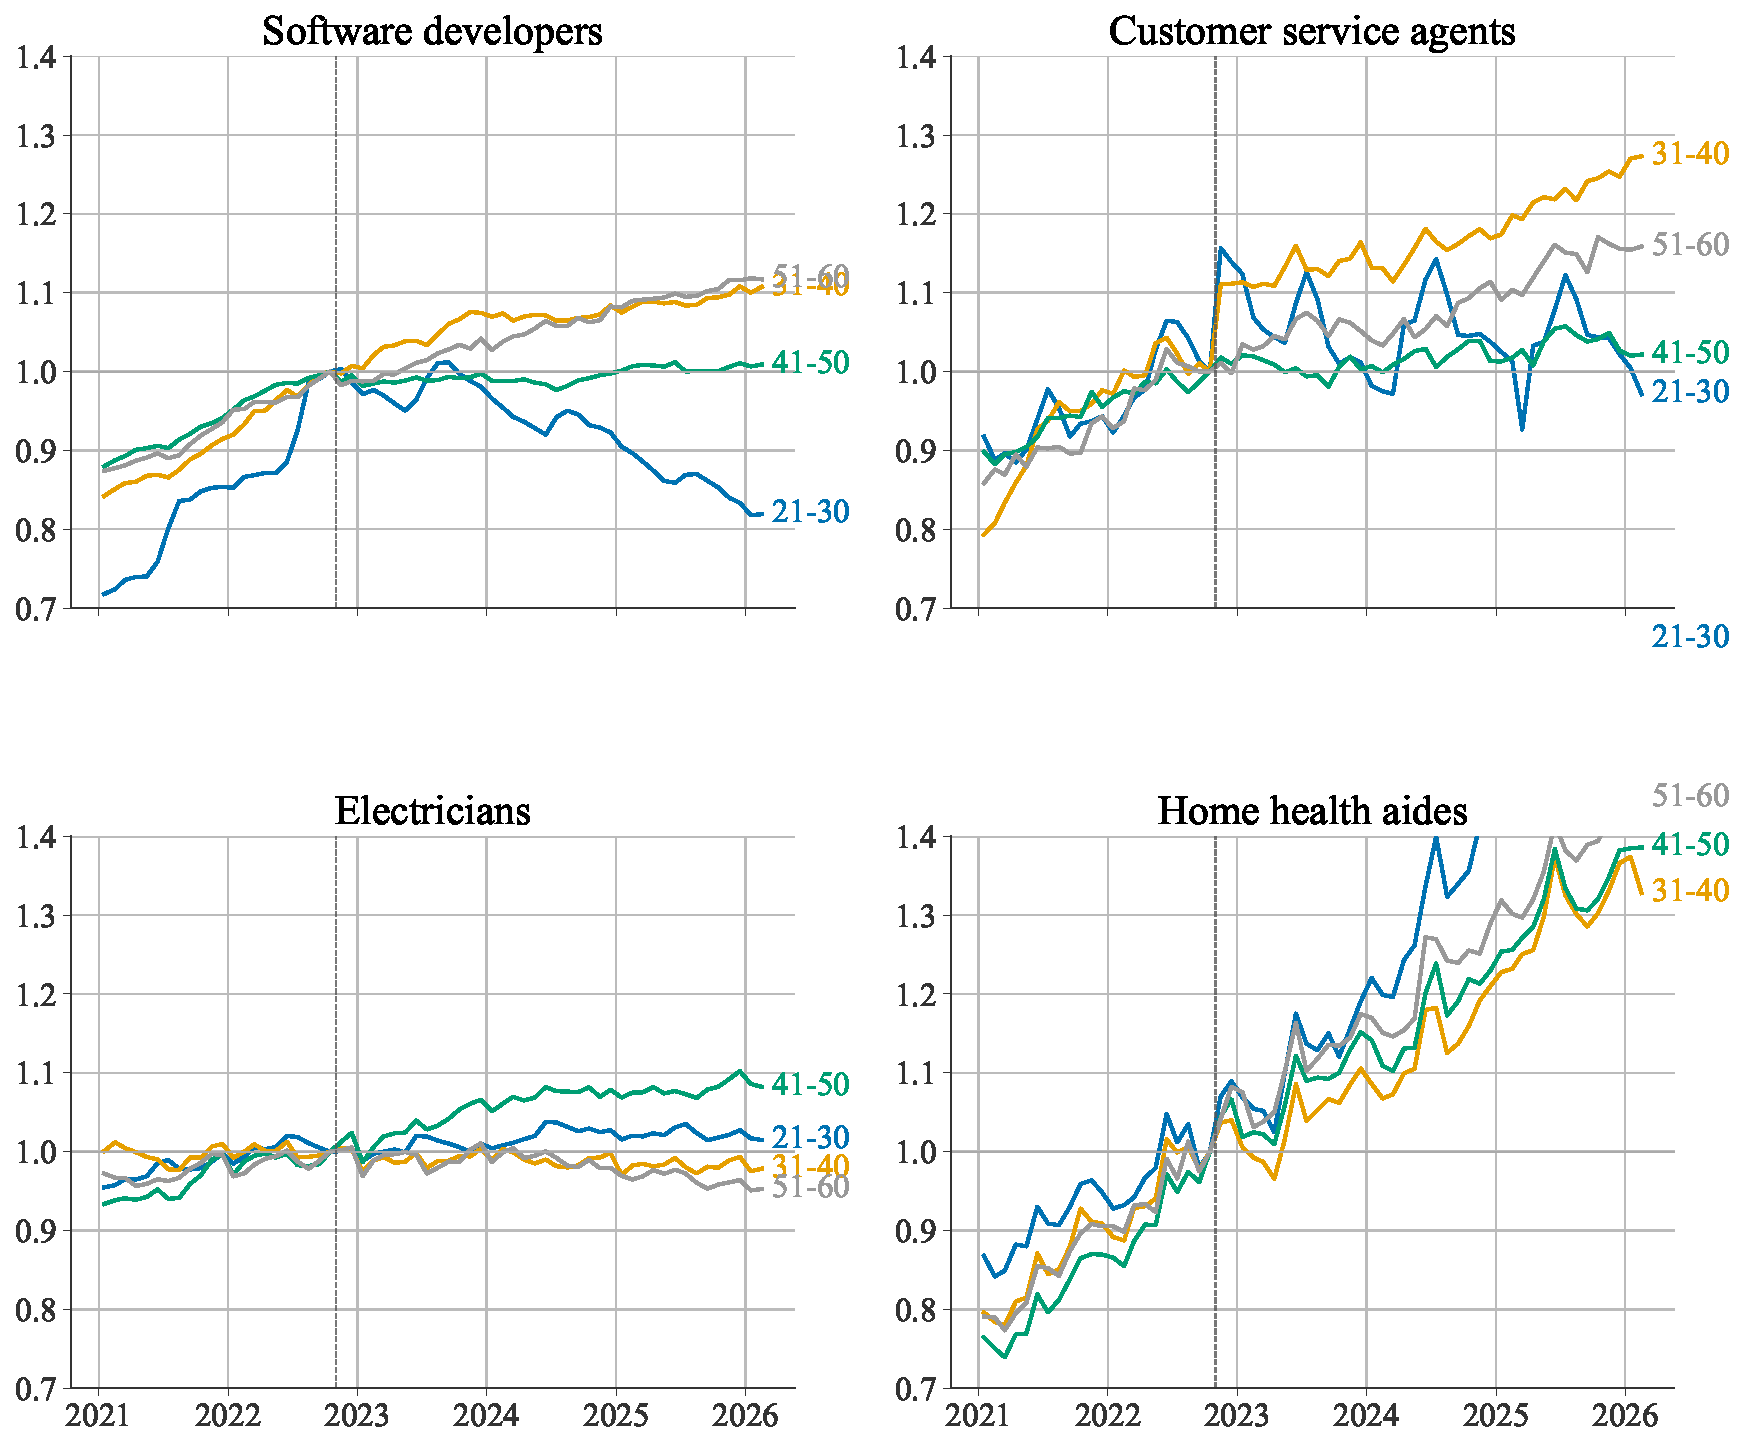
\includegraphics[width=\textwidth]{../analysis/output/figures/figure1_occupations_by_age.pdf}
  \caption{Employment in selected occupations, by decade age group.}
  \label{fig:occupations_by_age}
  \begin{minipage}{\textwidth}\footnotesize\textit{Notes:} Private-sector employment per capita (headcount divided by resident population in the age group), indexed to October 2022 = 1. Panels show the kiindeksen.no case-study occupations: software developers (STYRK-08 2512--2514, 2519) and customer service agents (4222), both high-exposure, and electricians (7411) and home health aides (5322), both low-exposure. The vertical dashed line marks November 30, 2022 (ChatGPT release).\end{minipage}
\end{figure}


\subsection{Employment by AI Exposure Quintile}\label{sec:results:quintiles}

The case studies above examine occupations chosen for their AI relevance. A more systematic approach ranks all occupations by their AI exposure score and examines whether high-exposure occupations exhibit different employment trends than low-exposure occupations. We assign each occupation to a quintile based on its Eloundou et al.\ GPT-4 exposure score, from Q1 (least exposed) to Q5 (most exposed), and plot normalized employment by quintile within each age group.

Figure~\ref{fig:age_by_quintile} plots quintile-by-age employment for the private sector, indexed to October 2022. Each of the four panels is one decade age group, with quintile lines running from light blue (Q1, least exposed) to dark blue (Q5, most exposed) and a red line for the overall age-group trend.

The most-exposed occupations do not lose ground among the youngest workers: in the 21--30 group the Q5 series tracks Q1 after the ChatGPT release, so the systematic exposure ranking does not reproduce the decline seen in the selected occupations. Among the older groups the Q5 series runs above Q1 at 31--40, ends a few points below at 41--50, and shows no clear separation at 51--60; these older movements are smaller than the pre-period swings discussed in Section~\ref{sec:robustness:pretrends}.


\begin{figure}[tp]
  \centering
  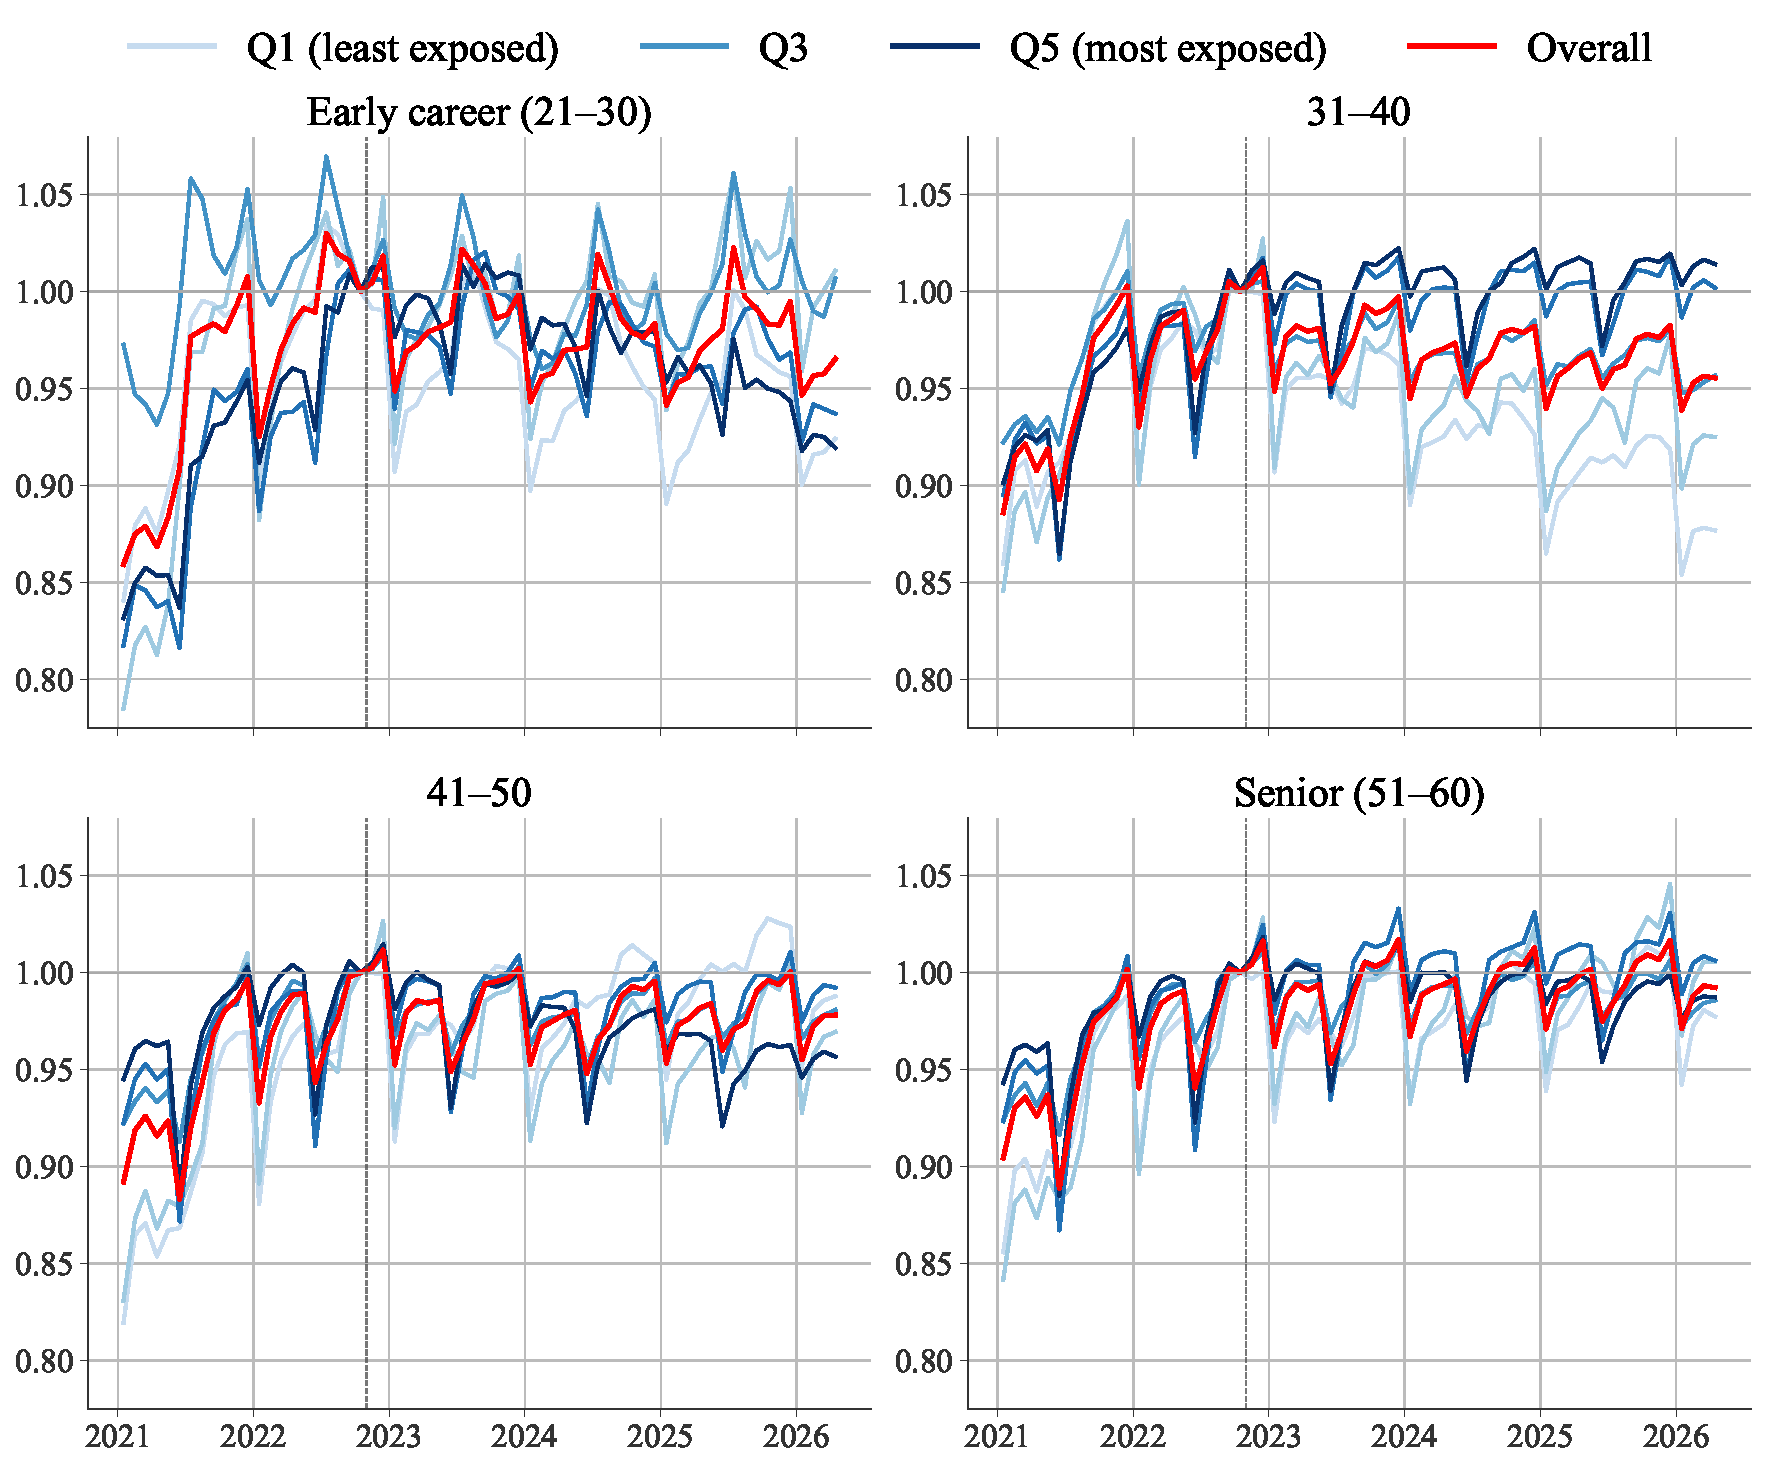
\includegraphics[width=\textwidth]{../analysis/output/figures/figure_emp_decade_private.pdf}
  \caption{Employment by AI-exposure quintile and decade age group, private sector.}
  \label{fig:age_by_quintile}
  \begin{minipage}{\textwidth}\footnotesize\textit{Notes:} Private-sector employment per capita (headcount divided by resident population in the age group), indexed to October 2022 = 1. Occupations are ranked by the Eloundou et al.\ GPT-4 exposure score. Q1 (lightest) = least exposed; Q5 (darkest) = most exposed. Red line = overall age-group trend. Vertical dashed line marks the November 2022 ChatGPT release.\end{minipage}
\end{figure}


The companion automation and augmentation quintile plots based on the Handa et al.\ decomposition are reported in Appendix Figures~\ref{fig:age_by_quintile_handa_auto} and~\ref{fig:age_by_quintile_handa_aug}.


\subsection{Seasonal Adjustment}\label{sec:results:sa}

Norwegian employment series carry a strong seasonal pattern, with a January dip and a summer peak. The figures above plot the series without seasonal adjustment, which is adequate for visual comparison over multi-year horizons but folds the calendar-month pattern into any short-horizon comparison. To match the seasonally adjusted series shown on the companion dashboard, we reproduce the main employment figures after removing a frozen seasonal component.

The adjustment is a transparent X-11 core, applied to each series in logs: the trend is a centred $2\times12$ moving average (thirteen months, half weight on the two endpoints), the seasonal factor for each calendar month is the average log-deviation from trend over January 2021--December 2024, and these factors are then frozen and subtracted from every month. Freezing the factors on the pre-2025 window keeps any later AI-related movement from leaking into the seasonal pattern. This is the same procedure used for the seasonally adjusted series on kiindeksen.no.

Figure~\ref{fig:byexposure_sa} shows seasonally adjusted employment by exposure quintile pooled over ages 21--60, and Figure~\ref{fig:age_by_quintile_sa} gives the adjusted decade-age panels alongside the raw panels of Figure~\ref{fig:age_by_quintile}. The adjusted series tell the same story as the raw ones: the most-exposed quintile does not separate clearly from the least-exposed.

\begin{figure}[tp]
  \centering
  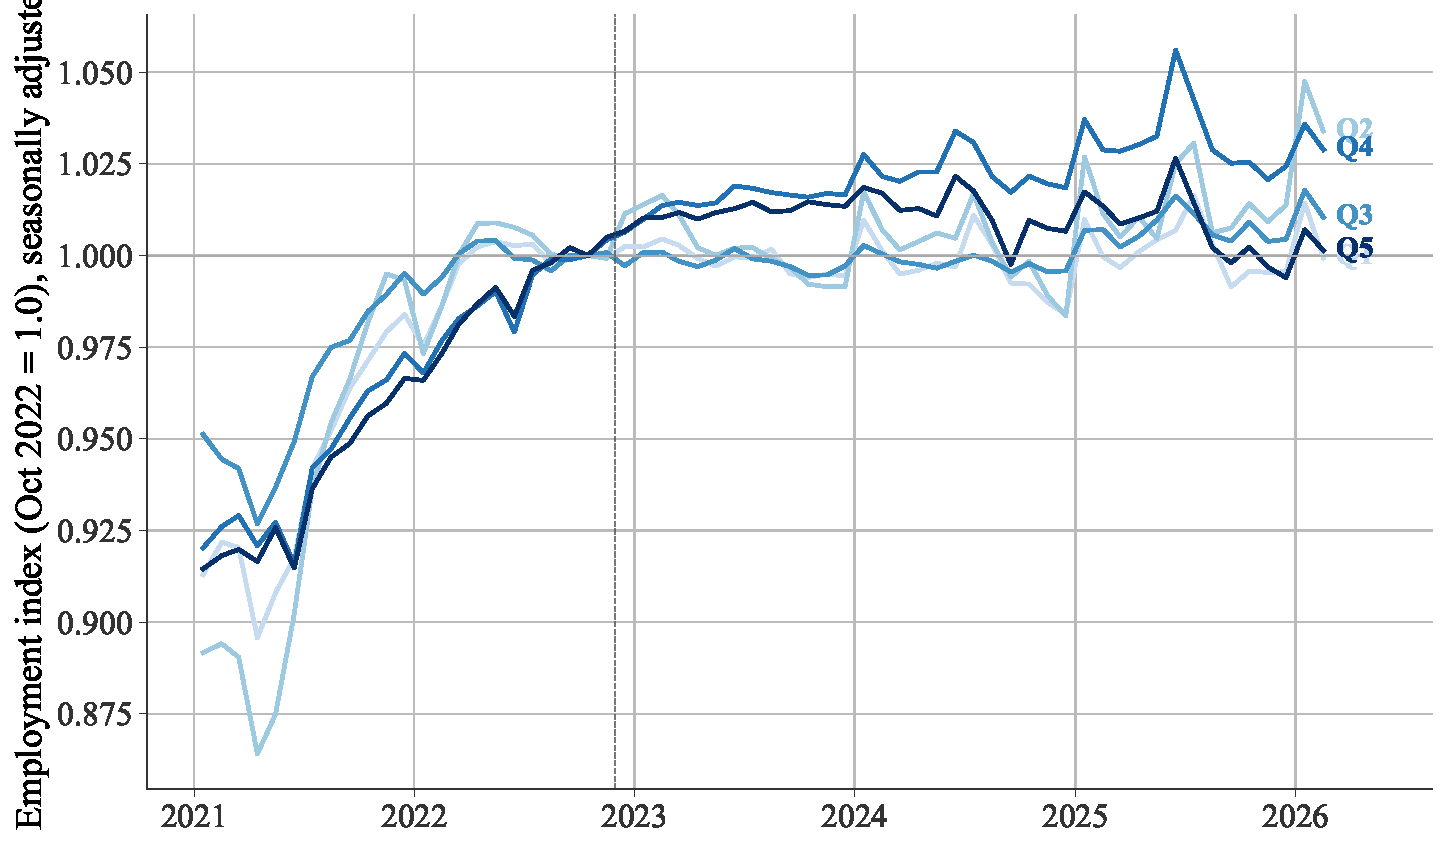
\includegraphics[width=0.8\textwidth]{../analysis/output/figures/figure_emp_byexposure_sa.pdf}
  \caption{Employment by AI-exposure quintile, all ages 21--60, private sector, seasonally adjusted.}
  \label{fig:byexposure_sa}
  \begin{minipage}{\textwidth}\footnotesize\textit{Notes:} Private-sector headcount pooled over ages 21--60, seasonally adjusted with a frozen X-11 core (factors estimated 2021--2024), indexed to October 2022 = 1. Occupations are ranked by the Eloundou et al.\ GPT-4 exposure score. This is the paper analog of the kiindeksen.no headline ``Sysselsetting etter KI-eksponering'' figure.\end{minipage}
\end{figure}

\begin{figure}[tp]
  \centering
  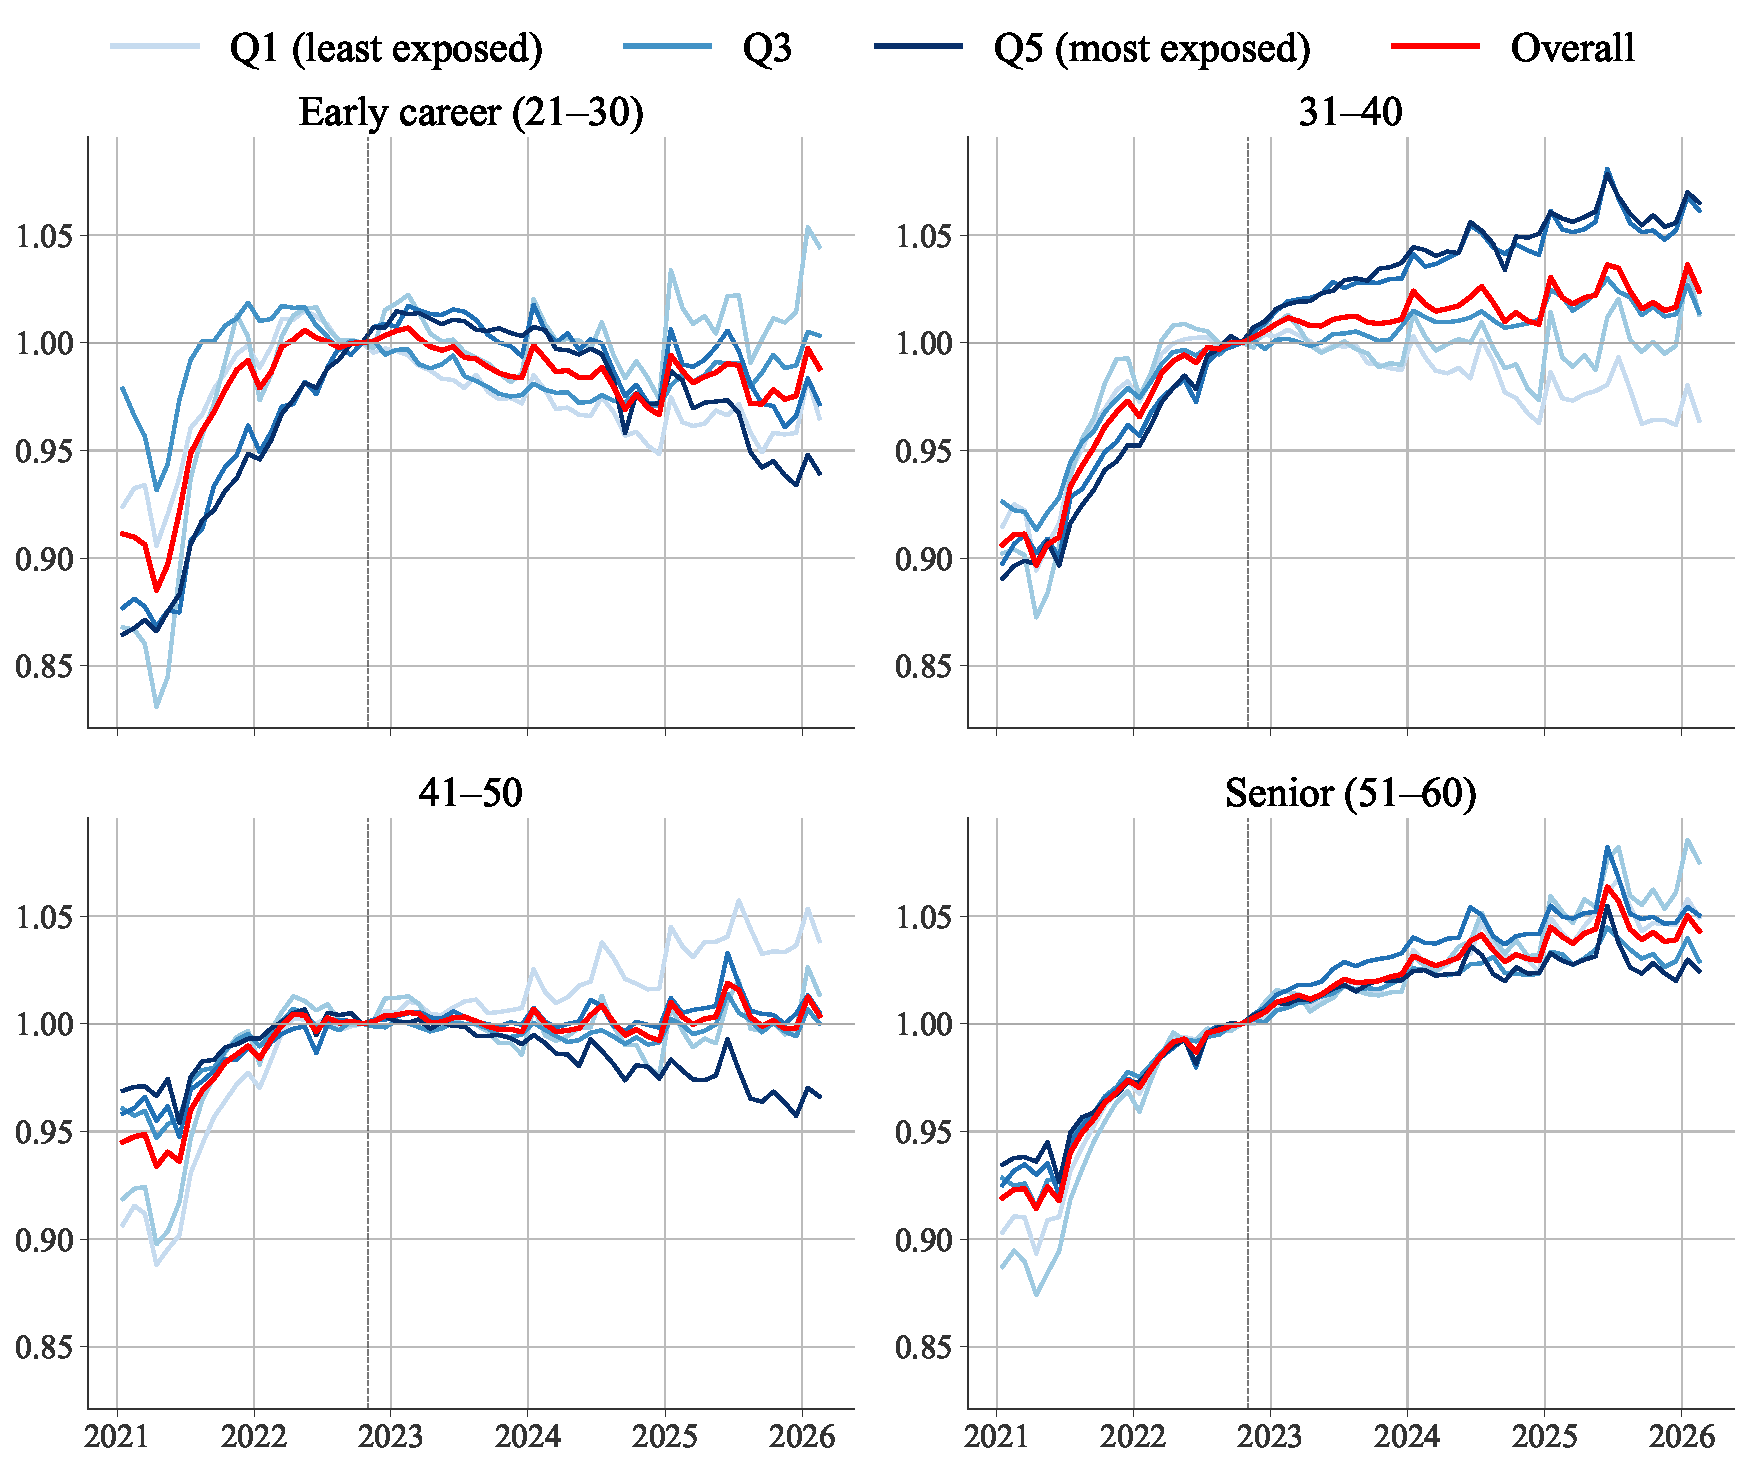
\includegraphics[width=\textwidth]{../analysis/output/figures/figure_emp_decade_private_sa.pdf}
  \caption{Employment by AI-exposure quintile and decade age group, private sector, seasonally adjusted.}
  \label{fig:age_by_quintile_sa}
  \begin{minipage}{\textwidth}\footnotesize\textit{Notes:} Seasonally adjusted headcount, the adjusted analog of Figure~\ref{fig:age_by_quintile} (which plots the unadjusted per-capita series); frozen X-11 adjustment with factors estimated 2021--2024, indexed to October 2022 = 1. Q1 (lightest) = least exposed; Q5 (darkest) = most exposed.\end{minipage}
\end{figure}


\subsection{Automation versus Augmentation}\label{sec:results:auto_aug}

We follow \citet{brynjolfsson2025} on the automation-vs-augmentation split. Ranking the youngest workers by Handa automation share gives a modest negative gradient (Appendix Figure~\ref{fig:age_by_quintile_handa_auto}); ranking them by augmentation share gives no gradient at all (Appendix Figure~\ref{fig:age_by_quintile_handa_aug}). This pattern is more consistent with automation than with augmentation, but the Handa classification only captures conversation mode, not what workers actually do on the job. An occupation scored as ``automation-exposed'' through conversation mode may in practice use AI for augmentation.


\subsection{Sector Heterogeneity}\label{sec:results:sectors}

The exposure patterns documented in Figure~\ref{fig:age_by_quintile} are private-sector patterns. The public sector shows no exposure gradient in any age group, in either the raw (Appendix Figure~\ref{fig:emp_public}) or the seasonally adjusted series (Appendix Figure~\ref{fig:emp_public_sa}).

The public-sector null could reflect slower adoption, hiring insulated from market conditions, stronger employment protection, or a different occupational mix; we cannot separate these from the aggregate data. The adoption channel does have some support: \citet{riksrevisjonen2024} report that fewer than half of about 200 state agencies have any experience developing or using AI, under a definition that excludes off-the-shelf tools such as ChatGPT, so theoretical exposure in the public sector does not translate into implementation. The public sector is dominated by health, education, and administration; private high-exposure occupations cluster in IT, finance, and business services.


\subsection{Wages and Other Outcomes}\label{sec:results:wages}

Figure~\ref{fig:kontantlonn_by_quintile} displays monthly cash earnings by Eloundou et al.\ exposure quintile and age group. Strong seasonal patterns dominate the wage plots: June earnings rise to about 1.6 times the baseline because of statutory holiday pay, and December earnings to about 1.2 because of year-end bonuses. The indexed series show no divergence by exposure quintile, and the within-firm difference-in-differences estimates (Table~\ref{tab:did_firmfe}) show no large earnings movement. \citet{brynjolfsson2025} and \citet{humlum2026} find no wage divergence over a similar horizon in the US and Denmark. Norway's two-tier bargaining system \citep{bhuller2022} with sectoral wage floors and strong employment protection make the quantity margin the more likely site of adjustment.

Three additional outcomes are reported in the appendix: contracted position percentage (Figure~\ref{fig:stillingspst_by_quintile}), overtime hours (Figure~\ref{fig:overtid_by_quintile}), and the share of new jobs (Figure~\ref{fig:nyjobb_by_quintile}). None shows a differential trend by exposure quintile.

\begin{figure}[tp]
  \centering
  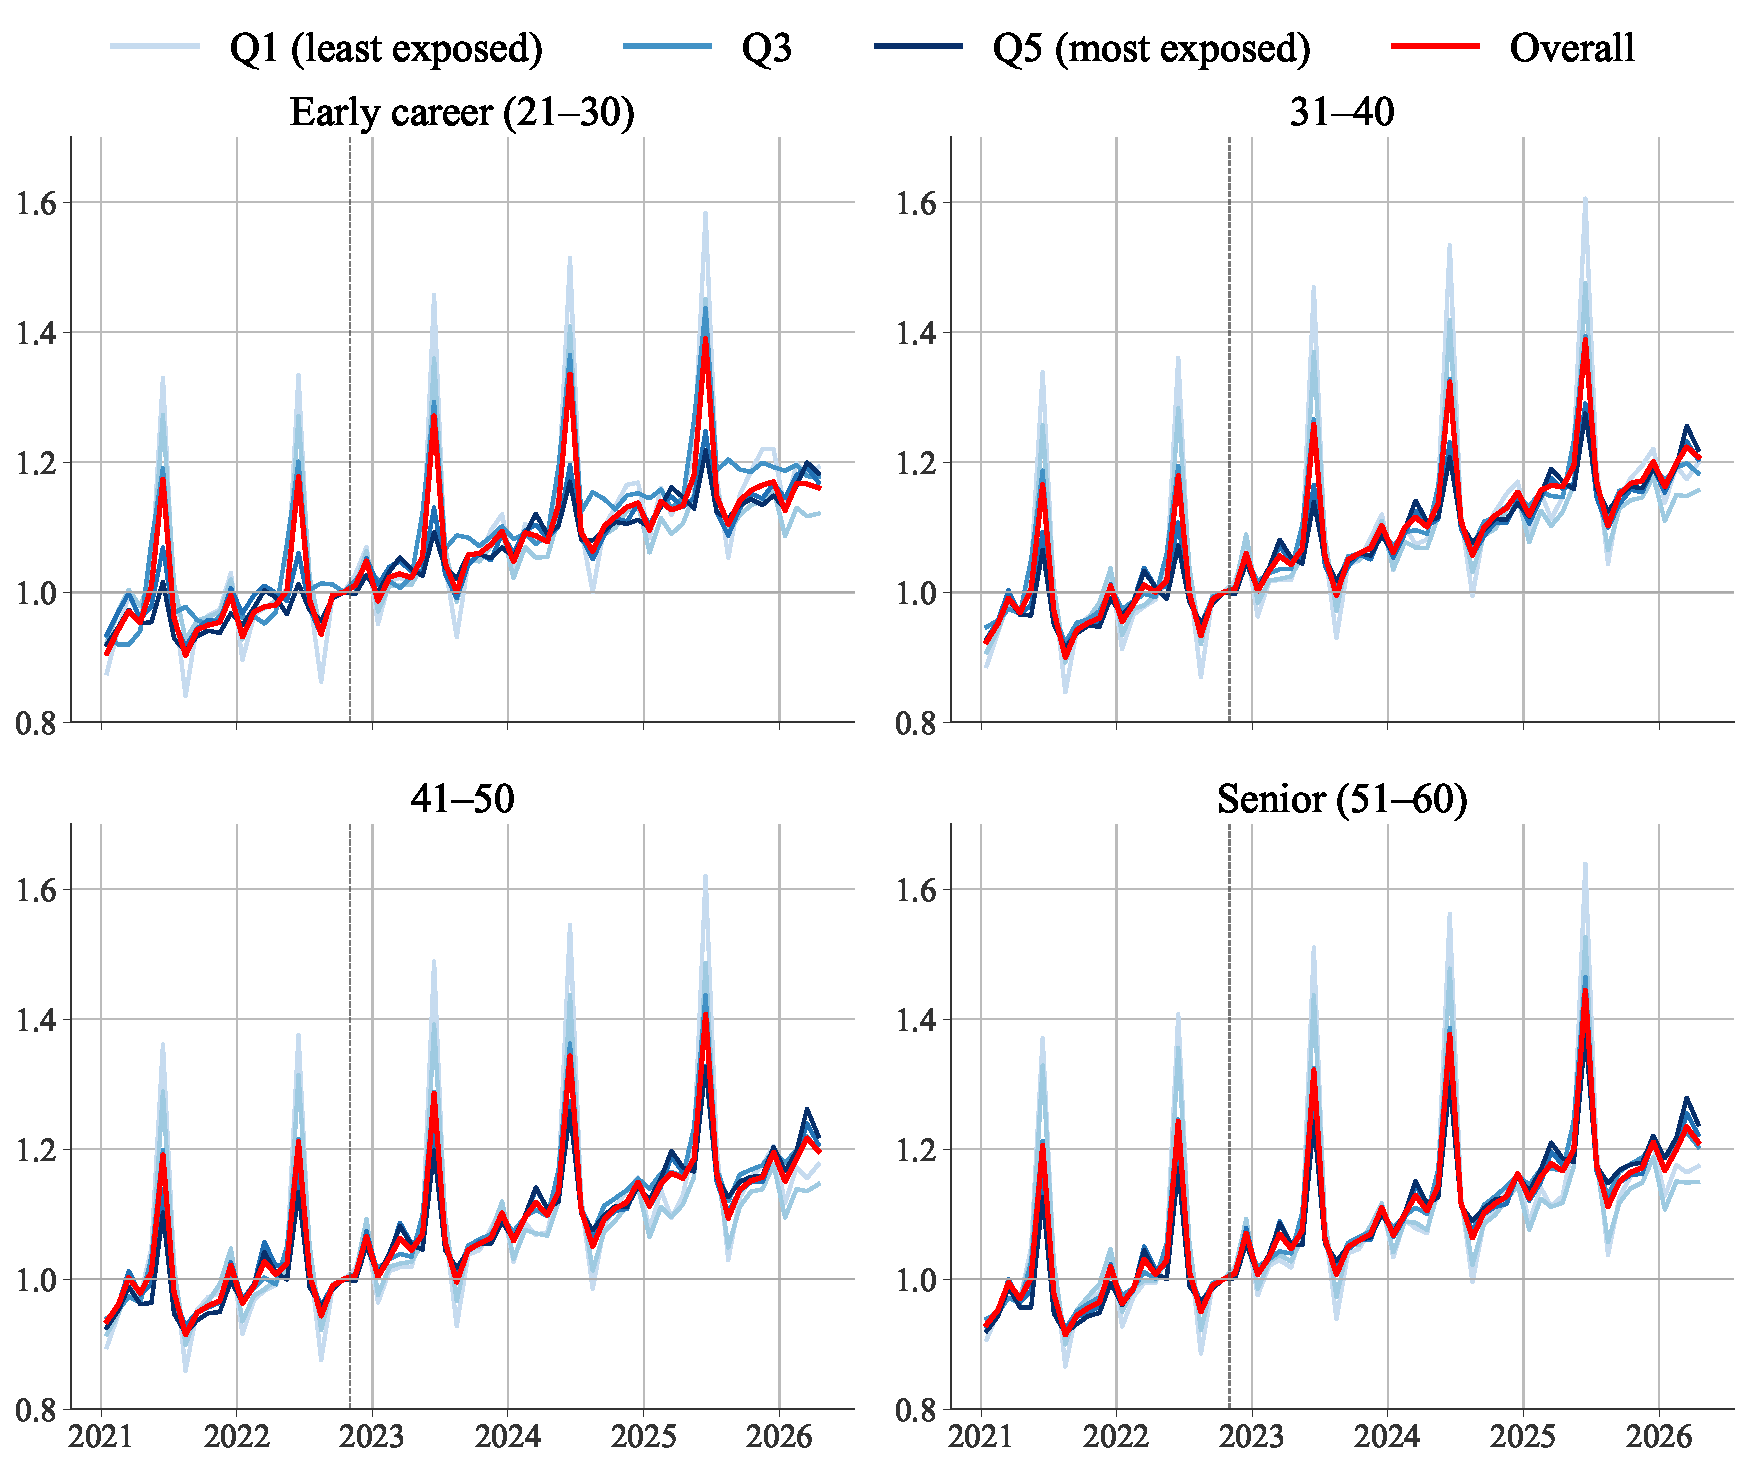
\includegraphics[width=\textwidth]{../analysis/output/figures/figure_kontantlonn_decade_private.pdf}
  \caption{Monthly cash earnings by AI-exposure quintile and decade age group, private sector.}
  \label{fig:kontantlonn_by_quintile}
  \begin{minipage}{\textwidth}\footnotesize\textit{Notes:} Mean monthly cash earnings, indexed to October 2022 = 1. Occupations are ranked by the Eloundou et al.\ exposure score. Strong seasonal patterns (December bonuses, June holiday pay) are visible in all panels.\end{minipage}
\end{figure}


% =============================================================================
\section{Regression Analysis}\label{sec:regression}

The descriptive series show little systematic separation across the exposure distribution. We summarize that cross-section here and then turn to the panel event studies. Table~\ref{tab:quintile_change} reports, for all private-sector workers aged 21--60, the mean employment change from October 2022 to the last month of data by exposure quintile, together with the Q5$-$Q1 ``double difference''. Each occupation is one observation, weighted by its October 2022 employment so the quintile means match the headcount aggregation used by the companion dashboard \citep{kiindeksen2026}; standard errors are heteroskedasticity-robust across occupations. On the seasonally adjusted series the double difference is essentially zero and statistically insignificant, so the most-exposed quintile has not grown differently from the least-exposed since ChatGPT. The raw series show a larger positive gap, but that reflects the October-versus-February calendar-month comparison that the seasonal adjustment removes.

\begin{table}[tp]
  \centering
  \caption{Employment change by AI-exposure quintile, October 2022 to February 2026, all ages 21--60, private sector.}
  \label{tab:quintile_change}
  \begin{tabular}{lcccccc}
\toprule
 & Q1 & Q2 & Q3 & Q4 & Q5 & Q5$-$Q1 \\
 & (least) &  &  &  & (most) & (DD) \\
\midrule
\multicolumn{7}{l}{\textit{Panel A. Seasonally adjusted}} \\
Change (\%) & +0.12 & +3.49 & +1.16 & +2.94$^{*}$ & +0.07 & -0.05 \\
 & (1.47) & (5.20) & (2.18) & (1.55) & (1.95) & (2.44) \\
\addlinespace
\multicolumn{7}{l}{\textit{Panel B. Raw}} \\
Change (\%) & -4.26$^{***}$ & -1.39 & -0.50 & +1.54 & -0.67 & +3.59 \\
 & (1.63) & (4.88) & (1.94) & (1.49) & (1.98) & (2.57) \\
\addlinespace
\midrule
Occupations & 78 & 73 & 78 & 79 & 76 & 384 \\
\bottomrule
\end{tabular}

  \begin{minipage}{\textwidth}\footnotesize\textit{Notes:} Each occupation's private-sector headcount change from October 2022 to the last month (February 2026), pooled over ages 21--60, regressed on exposure-quintile dummies and weighted by October 2022 employment, so the per-quintile means reproduce the headcount aggregation of the companion index. Panel~A uses the seasonally adjusted series (the same X-11 adjustment as the kiindeksen.no dashboard); Panel~B is unadjusted. ``Q5$-$Q1 (DD)'' is the double difference between the most- and least-exposed quintiles. Heteroskedasticity-robust standard errors in parentheses. $^{*}$, $^{**}$, $^{***}$ denote significance at the 10, 5, and 1 percent levels.\end{minipage}
\end{table}

Table~\ref{tab:did_cell} reports the corresponding difference-in-differences estimates: the average post-October-2022 change in each quintile relative to Q1 (the least-exposed quintile), by age group, for employment and new hires. For the youngest workers the most-exposed quintiles are not statistically distinguishable from Q1, and new hires show no systematic gradient in any age group. Among the older groups the employment estimate is positive at 31--40 (Q5 about $+0.078$ log points, $p<0.01$) and a small, insignificant negative at 41--50 ($-0.015$). Because pre-trends differ across these groups (Section~\ref{sec:robustness:pretrends}), we read these post-period summaries as descriptive. An insignificant estimate here is an absence of a detectable gradient, not evidence that exposure has no effect.

\begin{table}[tp]
  \centering
  \caption{Cell-level difference-in-differences by AI-exposure quintile, private sector.}
  \label{tab:did_cell}
  \begin{tabular}{lcccc}
\toprule
 & Early career & 31--40 & 41--50 & Senior \\
 & (21--30) &  &  & (51--60) \\
 & (1) & (2) & (3) & (4) \\
\midrule
\multicolumn{5}{l}{\textit{Panel A. Employment (Poisson)}} \\
Q2 $\times$ Post & 0.0428 & 0.0181 & -0.0206 & 0.0080 \\
 & (0.0341) & (0.0357) & (0.0339) & (0.0268) \\
Q3 $\times$ Post & 0.0449$^{**}$ & 0.0432$^{***}$ & -0.0049 & 0.0102 \\
 & (0.0204) & (0.0167) & (0.0153) & (0.0135) \\
Q4 $\times$ Post & 0.0193 & 0.0707$^{***}$ & 0.0000 & 0.0216 \\
 & (0.0203) & (0.0169) & (0.0154) & (0.0134) \\
Q5 $\times$ Post & 0.0215 & 0.0783$^{***}$ & -0.0146 & 0.0103 \\
 & (0.0220) & (0.0186) & (0.0169) & (0.0166) \\
\addlinespace
\multicolumn{5}{l}{\textit{Panel B. New hires (Poisson)}} \\
Q2 $\times$ Post & 0.1247 & 0.2475$^{**}$ & 0.1836 & 0.2422$^{*}$ \\
 & (0.0810) & (0.1223) & (0.1247) & (0.1452) \\
Q3 $\times$ Post & 0.1158 & 0.1775$^{*}$ & 0.0999 & 0.0657 \\
 & (0.0740) & (0.1019) & (0.1100) & (0.1129) \\
Q4 $\times$ Post & 0.0713 & 0.1303 & 0.0591 & -0.0043 \\
 & (0.0770) & (0.1024) & (0.1074) & (0.1190) \\
Q5 $\times$ Post & -0.0424 & 0.0160 & -0.0116 & 0.0200 \\
 & (0.0845) & (0.1054) & (0.1104) & (0.1122) \\
\midrule
Occupations & 393 & 391 & 393 & 392 \\
Observations (count) & 24,366 & 24,242 & 24,366 & 24,304 \\
\bottomrule
\end{tabular}

  \begin{minipage}{\textwidth}\footnotesize\textit{Notes:} Each entry is the post-October-2022 change in the indicated quintile relative to Q1 (least exposed), by decade age group. Employment and new hires are Poisson. Occupation and month fixed effects; standard errors clustered by occupation. Sample 2021m1--2026m2. $^{*}$, $^{**}$, $^{***}$ denote $p<0.1$, $0.05$, $0.01$.\end{minipage}
\end{table}


\subsection{Poisson Regression Estimates}\label{sec:results:firmfe}

The quintile series so far normalize employment by the population in each age group, the right denominator for asking whether cohort-level employment shifts away from AI-exposed occupations. We turn now to the worker counts and ask whether they reallocate across occupations. Following \citet{brynjolfsson2025}, we estimate Poisson event studies on the counts.

The cell-level microdata are tabulated at the (occupation $\times$ age group $\times$ month) level. We estimate
\[
\log E[\text{count}_{j,a,t}] = \alpha_{j} + \beta_{t} + \gamma_{q,k},
\]
separately per decade age group~$a$ in the private sector, where $j$ indexes occupations and $q(j)$ is the Eloundou GPT-4 $\beta$ quintile of occupation~$j$. The occupation FE absorbs the permanent employment level of each occupation; the month FE absorbs the aggregate time path of the age cohort. Standard errors are clustered at occupation. Reference: Q1 and $k=-1$ (October 2022).

Figure~\ref{fig:microdata_poisson_grid} reports the resulting $\gamma_{q,k}$ for $q\in\{2,3,4,5\}$ across the four decade age groups, in log points. The path matches the indexed series in Figure~\ref{fig:age_by_quintile}. At 41--50 the Q5 path turns negative after October 2022, reaches about $-0.08$ log points by mid-2025, and ends near $-0.03$ by early 2026. At 21--30 the Q5 path is noisy and ends near zero; at 31--40 it rises to about $+0.15$; at 51--60 it stays near zero.

\begin{figure}[tp]
  \centering
  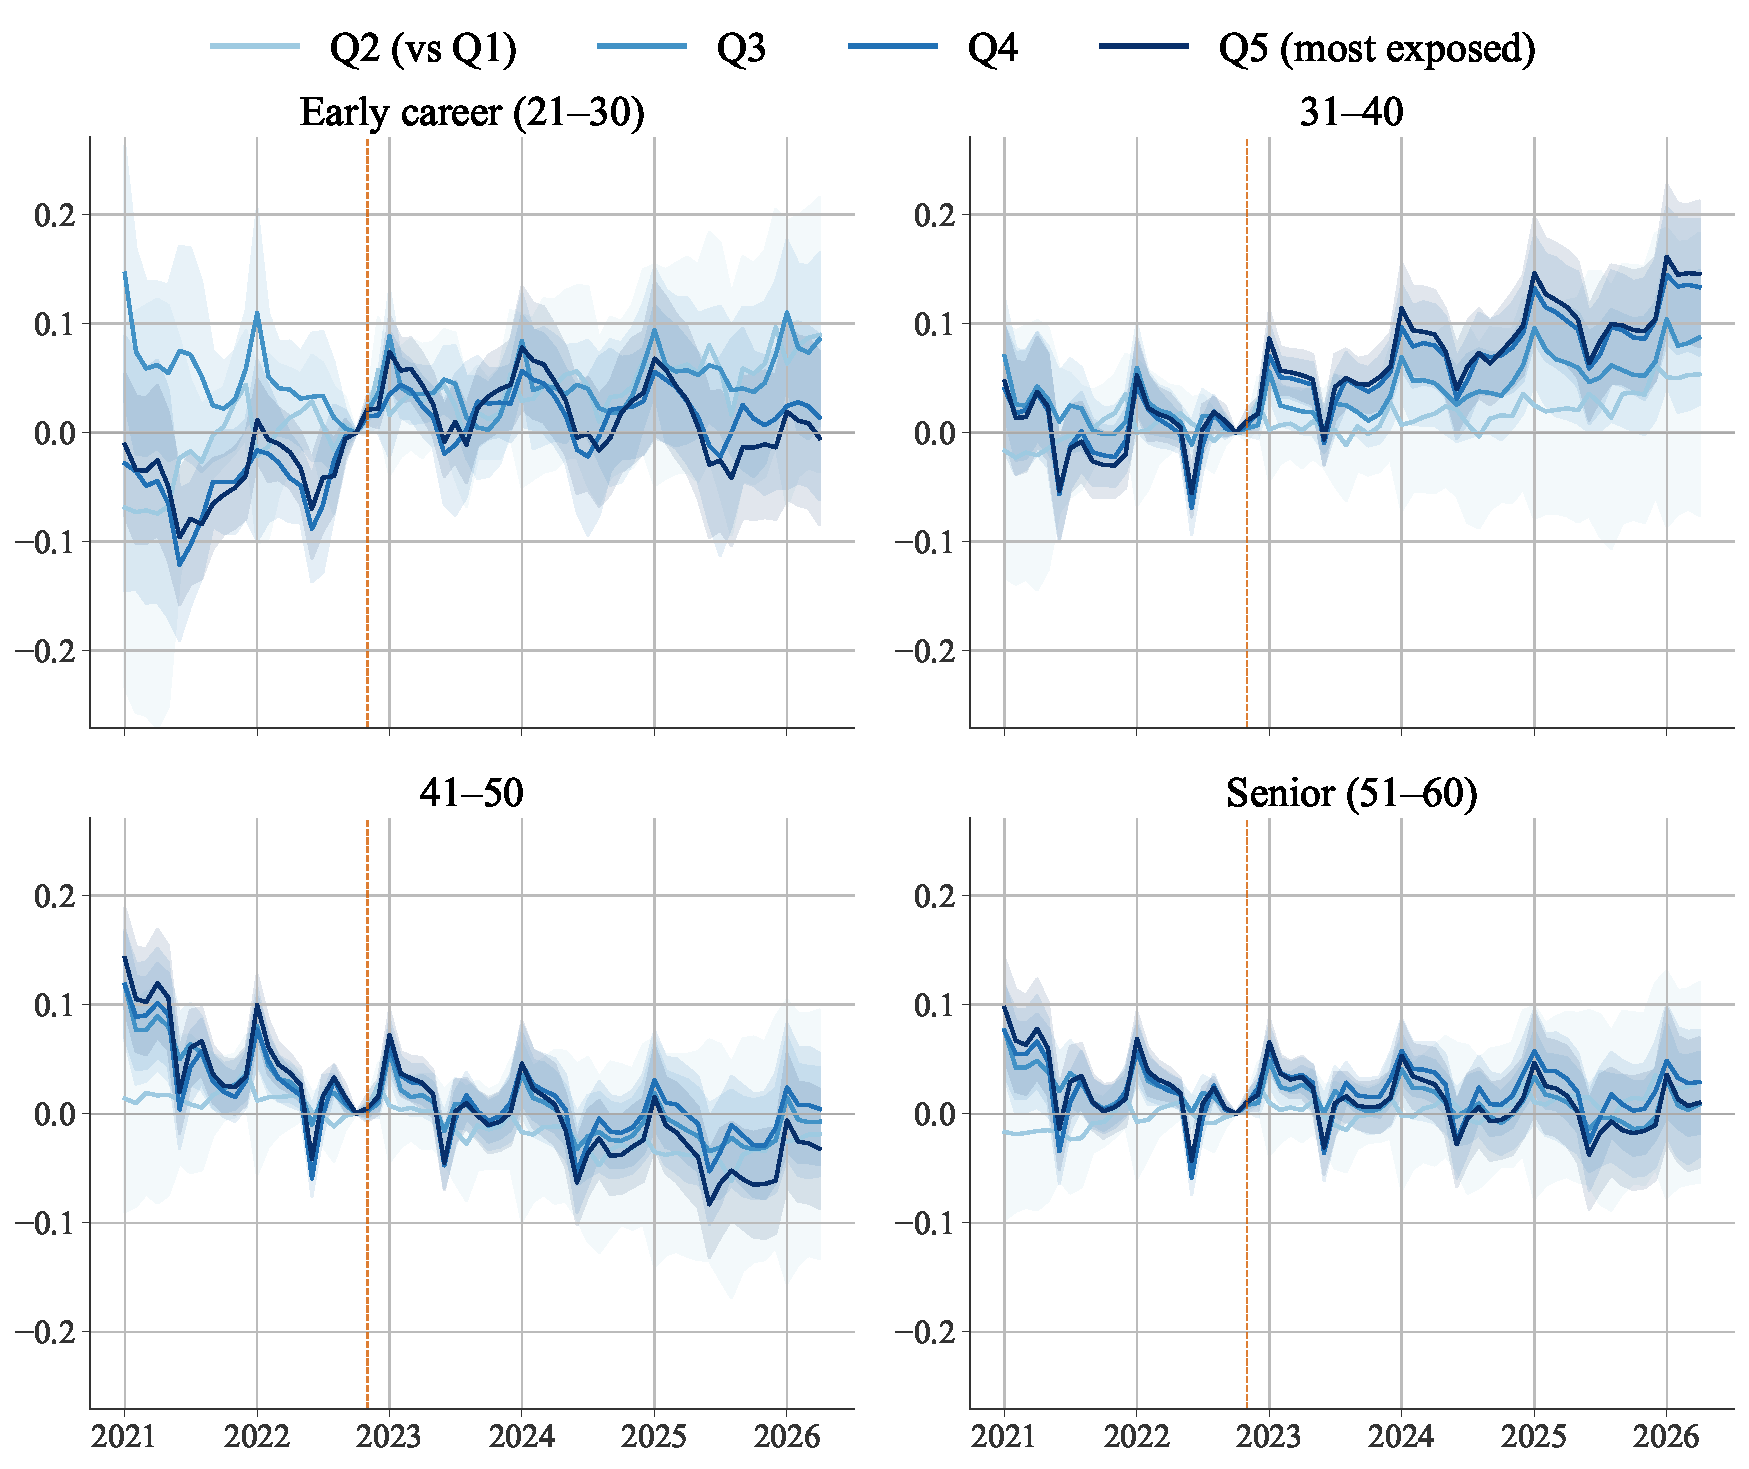
\includegraphics[width=\textwidth]{../analysis/output/figures/figure_microdata_poisson_es_grid.pdf}
  \caption{Poisson event-study coefficients by AI-exposure quintile and decade age group, private sector.}
  \begin{minipage}{\textwidth}\footnotesize\textit{Notes:} Coefficients $\gamma_{q,k}$ for $q\in\{2,\dots,5\}$ relative to $q=1$, in log points. Cell-level microdata.no aggregates (occupation\,$\times$\,age\,$\times$\,month), private sector; fixed effects for occupation and month. Sample 2021m1--2026m2. Shaded bands: 95\% confidence intervals clustered at occupation. Reference: October 2022. Dashed line marks the November 2022 ChatGPT release.\end{minipage}
  \label{fig:microdata_poisson_grid}
\end{figure}

The cell-level estimates absorb the average employment path of each occupation but do not separate reallocation \emph{within} firms from changes in the firm composition. Using the individual-level records, we estimate the within-firm composition design of \citet{brynjolfsson2025},
\[
\log E[\text{count}_{f,q,a,t}] = \alpha_{f,q} + \beta_{f,t} + \gamma_{q,k},
\]
on the panel of firm $f$ $\times$ quintile $q$ $\times$ month $t$ cells, separately per decade age group. Firm-by-quintile and firm-by-month fixed effects absorb the firm's persistent composition and any firm-level demand shock; identification rests on within-firm reallocation across exposure quintiles. Standard errors are clustered at the firm. The sample is private-sector \emph{foretak} with at least 20 workers in the 21--60 age window per month, January 2021 through February 2026.

Figure~\ref{fig:firmfe_poisson_grid} reports the firm-FE $\gamma_{q,k}$. For the youngest workers the Q5 path is noisy and ends slightly positive, so the within-firm comparison, like the cell-level one, does not show the most-exposed quintile penalizing the young. The older groups line up with the cell-level estimates: at 31--40 the Q5 path rises to about $+0.12$, at 41--50 it drifts negative through 2025 and recovers to near zero by early 2026, and at 51--60 it stays near zero. The collapsed within-firm estimates in Table~\ref{tab:did_firmfe} match this reading: the Q5 employment coefficient is not distinguishable from zero at 21--30, positive at 31--40 ($+0.051$, $p<0.01$), marginally negative at 41--50 ($-0.021$, $p<0.1$), and near zero at 51--60. New hires show no systematic exposure gradient.

\begin{figure}[tp]
  \centering
  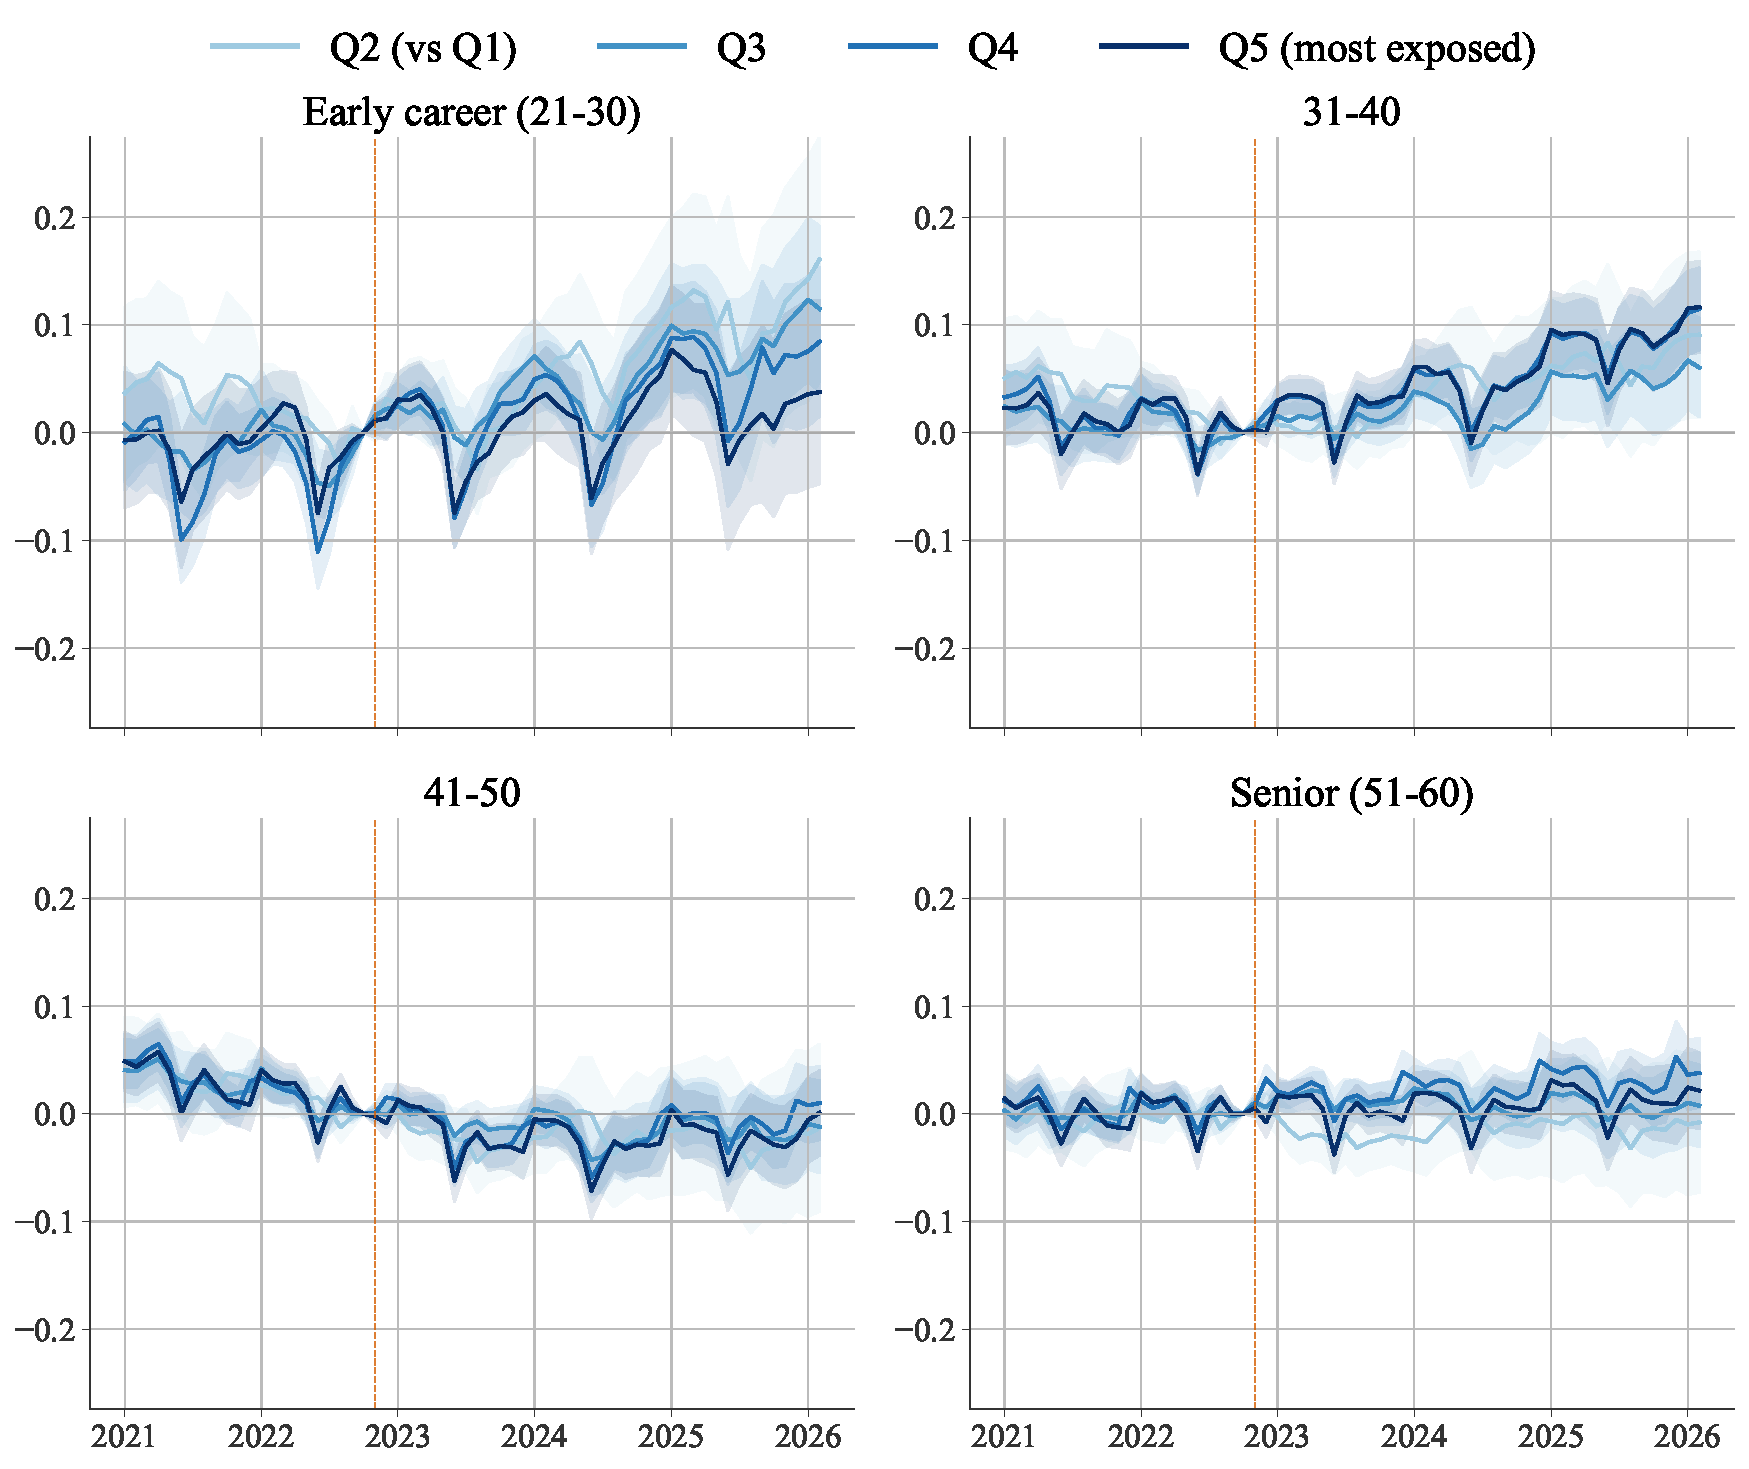
\includegraphics[width=\textwidth]{../analysis/output/figures/figure_firmfe_poisson_es_grid.pdf}
  \caption{Firm-fixed-effects Poisson event-study coefficients by AI-exposure quintile and decade age group, private sector.}
  \begin{minipage}{\textwidth}\footnotesize\textit{Notes:} Coefficients $\gamma_{q,k}$ for $q\in\{2,\dots,5\}$ relative to $q=1$, in log points. Estimated on the individual-level firm $\times$ quintile $\times$ month panel; fixed effects for firm $\times$ quintile and firm $\times$ month. Private-sector foretak with at least 20 workers in the 21--60 age window per month. Sample 2021m1--2026m2. Shaded bands: 95\% confidence intervals clustered at the firm. Reference: October 2022. Dashed line marks the November 2022 ChatGPT release.\end{minipage}
  \label{fig:firmfe_poisson_grid}
\end{figure}

\begin{table}[tp]
  \centering
  \caption{Within-firm difference-in-differences by AI-exposure quintile, private sector.}
  \label{tab:did_firmfe}
  \begin{tabular}{lcccc}
\toprule
 & Early career & 31--40 & 41--50 & Senior \\
 & (21--30) &  &  & (51--60) \\
 & (1) & (2) & (3) & (4) \\
\midrule
\multicolumn{5}{l}{\textit{Panel A. Employment (Poisson)}} \\
Q2 $\times$ Post & 0.0611$^{**}$ & 0.0403$^{**}$ & -0.0190 & -0.0125 \\
 & (0.0276) & (0.0205) & (0.0194) & (0.0169) \\
Q3 $\times$ Post & 0.0481$^{***}$ & 0.0252$^{**}$ & -0.0124 & 0.0088 \\
 & (0.0184) & (0.0125) & (0.0113) & (0.0107) \\
Q4 $\times$ Post & 0.0281$^{*}$ & 0.0506$^{***}$ & -0.0125 & 0.0249$^{***}$ \\
 & (0.0161) & (0.0108) & (0.0095) & (0.0089) \\
Q5 $\times$ Post & 0.0132 & 0.0511$^{***}$ & -0.0207$^{*}$ & 0.0071 \\
 & (0.0210) & (0.0122) & (0.0108) & (0.0096) \\
\addlinespace
\multicolumn{5}{l}{\textit{Panel B. New hires (Poisson)}} \\
Q2 $\times$ Post & 0.0117 & 0.0386 & -0.0100 & 0.1022 \\
 & (0.0991) & (0.0940) & (0.1032) & (0.1230) \\
Q3 $\times$ Post & 0.0456 & -0.0365 & -0.0228 & -0.0899 \\
 & (0.1011) & (0.0902) & (0.0913) & (0.1108) \\
Q4 $\times$ Post & 0.0374 & 0.1243 & -0.0222 & -0.0493 \\
 & (0.1227) & (0.0942) & (0.1007) & (0.1236) \\
Q5 $\times$ Post & -0.0031 & 0.0318 & -0.0516 & -0.2350$^{*}$ \\
 & (0.1146) & (0.1130) & (0.1229) & (0.1374) \\
\addlinespace
\multicolumn{5}{l}{\textit{Panel C. Log monthly earnings (OLS)}} \\
Q2 $\times$ Post & -0.0140$^{*}$ & 0.0003 & -0.0010 & 0.0039 \\
 & (0.0085) & (0.0058) & (0.0056) & (0.0058) \\
Q3 $\times$ Post & -0.0041 & 0.0075 & 0.0065 & 0.0044 \\
 & (0.0072) & (0.0048) & (0.0045) & (0.0045) \\
Q4 $\times$ Post & -0.0059 & 0.0097$^{**}$ & 0.0187$^{***}$ & 0.0199$^{***}$ \\
 & (0.0072) & (0.0049) & (0.0044) & (0.0046) \\
Q5 $\times$ Post & 0.0021 & 0.0162$^{***}$ & 0.0180$^{***}$ & 0.0128$^{***}$ \\
 & (0.0081) & (0.0053) & (0.0047) & (0.0050) \\
\midrule
Firms & 21,842 & 21,893 & 21,769 & 21,246 \\
Observations & 2,223,802 & 2,420,283 & 2,439,058 & 2,313,496 \\
\bottomrule
\end{tabular}

  \begin{minipage}{\textwidth}\footnotesize\textit{Notes:} Each entry is the post-October-2022 change in the indicated quintile relative to Q1 (least exposed), by decade age group. Estimated on the individual-level firm $\times$ quintile $\times$ month panel; firm-by-quintile and firm-by-month fixed effects. Employment and new hires are Poisson; log monthly earnings is OLS. Private-sector foretak with at least 20 workers in the 21--60 age window per month. Sample 2021m1--2026m2. Standard errors clustered at the firm. $^{*}$, $^{**}$, $^{***}$ denote $p<0.1$, $0.05$, $0.01$.\end{minipage}
\end{table}


\subsection{Reconciling the Cell and Individual-Level Estimates}\label{sec:results:reconcile}

The cell-level estimates use microdata.no aggregates; the firm-FE estimates use the individual records on the secure server (universe 1191). The data source, the sample, and the specification all differ between the two, so we reconcile them in nested steps. Table~\ref{tab:validation} reports the Q5-vs-Q1 post-October-2022 employment coefficient under four specifications: (1) the microdata.no cell spec; (2) the same cell spec on the individual records, all private foretak; (3) the cell spec on foretak with at least 20 workers; and (4) the firm-FE spec on that restricted sample. Step (1) to (2) changes only the data source, (2) to (3) adds the size restriction, and (3) to (4) changes the specification. The samples in (3) and (4) are identical, verified cell by cell.

The estimate is stable along the chain. The data source contributes almost nothing: columns (1) and (2) differ by at most 0.003 log points in any age group. The size restriction moves the early-career coefficient from $+0.020$ to $+0.010$ and leaves the others within 0.01. The move from the cell to the firm-FE specification is the largest single step; it falls mainly on the 31--40 group, where the coefficient drops from $+0.085$ to $+0.051$, and on the 41--50 group, where the firm-FE estimate becomes marginally significant ($-0.021$, $p<0.1$). Signs are unchanged throughout. Figure~\ref{fig:cell_vs_firmfe} plots the cell and firm-FE event-study paths for Q5 together, and the two track each other in every age group. The microdata.no aggregates recover the same pattern as the individual records, and the within-firm specification does not overturn it.

\begin{table}[tp]
  \centering
  \caption{Cell-vs-individual reconciliation: Q5-vs-Q1 employment effect across nested specifications, private sector.}
  \label{tab:validation}
  \begin{tabular}{lcccc}
\toprule
 & microdata.no & \multicolumn{3}{c}{Individual records} \\
\cmidrule(lr){2-2}\cmidrule(lr){3-5}
 & cell & cell, all & cell, $\geq$20 & firm FE \\
 & (1) & (2) & (3) & (4) \\
\midrule
Early career & +0.0213 & +0.0202 & +0.0101 & +0.0126 \\
(21--30) & (0.0220) & (0.0214) & (0.0240) & (0.0210) \\
31--40 & +0.0782$^{***}$ & +0.0753$^{***}$ & +0.0843$^{***}$ & +0.0503$^{***}$ \\
 & (0.0185) & (0.0181) & (0.0197) & (0.0122) \\
41--50 & -0.0146 & -0.0159 & -0.0156 & -0.0206$^{*}$ \\
 & (0.0169) & (0.0168) & (0.0185) & (0.0108) \\
Senior & +0.0104 & +0.0081 & +0.0095 & +0.0074 \\
(51--60) & (0.0165) & (0.0160) & (0.0193) & (0.0096) \\
\bottomrule
\end{tabular}

  \begin{minipage}{\textwidth}\footnotesize\textit{Notes:} Each entry is the post-October-2022 change in employment for the most-exposed quintile (Q5) relative to the least-exposed (Q1), Poisson, by decade age group. Column (1) uses microdata.no cell aggregates (occupation $\times$ age $\times$ month, occupation and month fixed effects). Columns (2)--(4) use the individual records (universe 1191): (2) the same cell spec on all private foretak, (3) the cell spec on foretak with at least 20 workers in the 21--60 window, (4) the firm-FE spec (firm $\times$ quintile and firm $\times$ month fixed effects) on the same sample as (3). Standard errors in parentheses, clustered at occupation in (1)--(3) and at the firm in (4). Sample 2021m1--2026m2. $^{*}$, $^{**}$, $^{***}$ denote $p<0.1$, $0.05$, $0.01$.\end{minipage}
\end{table}

\begin{figure}[tp]
  \centering
  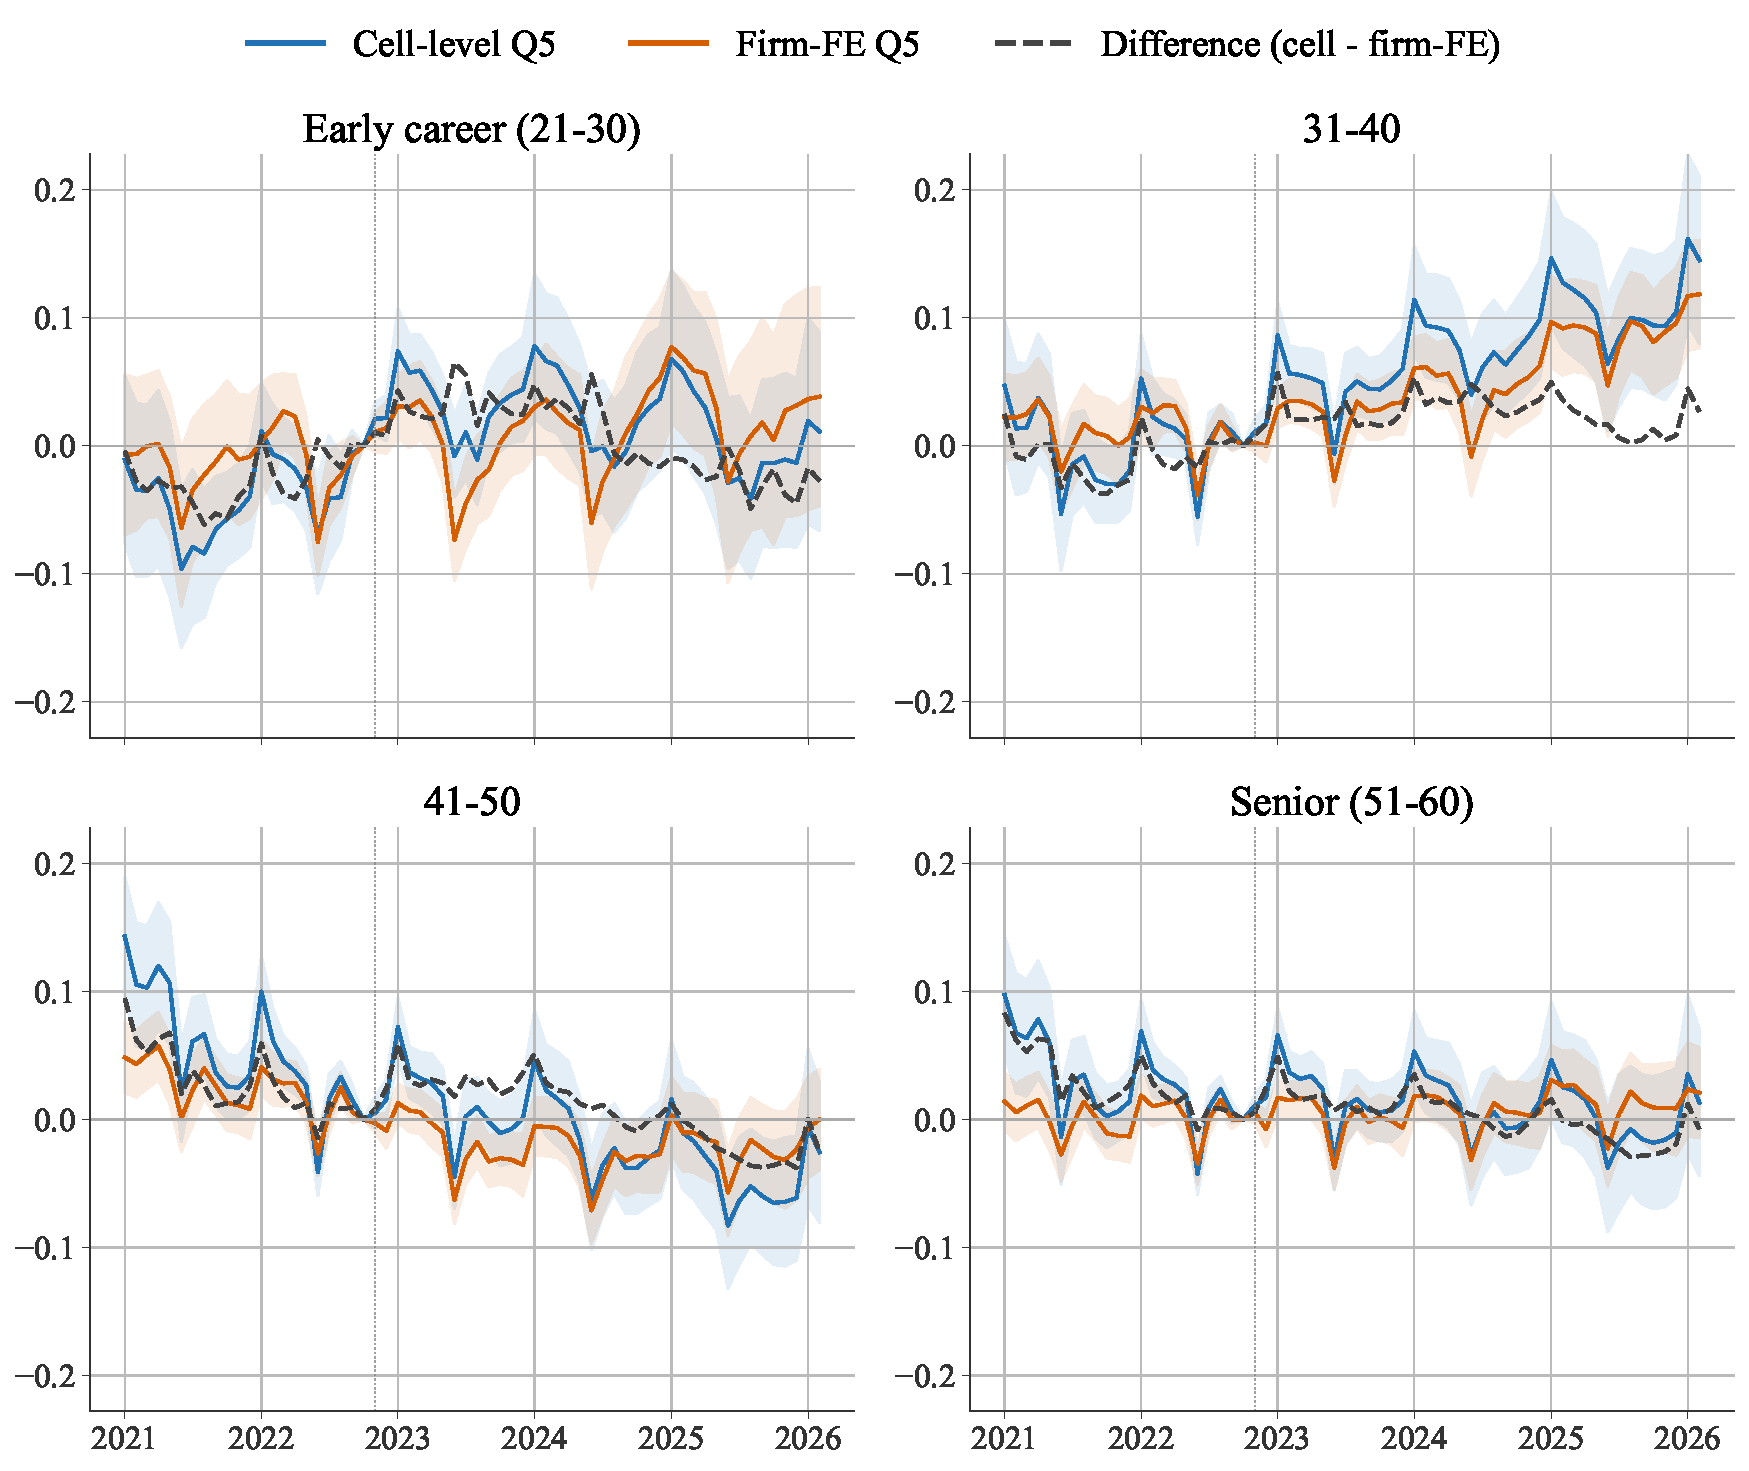
\includegraphics[width=\textwidth]{../analysis/output/figures/figure_cell_vs_firmfe_q5_grid.pdf}
  \caption{Cell-level and firm-FE event-study coefficients for the most-exposed quintile, by decade age group, private sector.}
  \label{fig:cell_vs_firmfe}
  \begin{minipage}{\textwidth}\footnotesize\textit{Notes:} Q5-vs-Q1 Poisson event-study coefficients, in log points, relative to October 2022. Blue: cell-level microdata.no spec (Figure~\ref{fig:microdata_poisson_grid}). Orange: individual-level firm-FE spec (Figure~\ref{fig:firmfe_poisson_grid}). Gray: cell minus firm-FE. Shaded bands: 95\% confidence intervals. Sample 2021m1--2026m2.\end{minipage}
\end{figure}


% =============================================================================

\subsection{Pre-Trends}\label{sec:robustness:pretrends}

The event studies in Section~\ref{sec:results:firmfe} display the pre-ChatGPT period, and the pre-period coefficients are not flat. In the cell-level event study the most-exposed quintile's pre-period path moves over a peak-to-trough range of 0.11 to 0.18 log points across the four age groups, as large as or larger than the post-2022 movements, and joint tests reject parallel pre-trends in every age group in both the cell and firm-FE specifications. The pre-period also differs across age groups and across occupations: software developers aged 21--30 are already declining before November 2022 (Figure~\ref{fig:occupations_by_age}), while other occupations are flat.

These pre-trends bear on interpretation. A difference-in-differences design, including the post-versus-pre estimates in Tables~\ref{tab:did_cell} and~\ref{tab:did_firmfe}, attributes the post-2022 change to the ChatGPT release under the assumption that the most- and least-exposed quintiles would otherwise have moved in parallel. That assumption is debatable here: the quintiles were already on diverging paths before November 2022, and the divergence differs by age group. A collapsed difference-in-differences can therefore read a continuation of a pre-existing trend as an AI effect, and the direction of the resulting bias need not be the same across age groups. We therefore treat the event studies as the primary evidence, read the difference-in-differences tables as summaries of the post-period rather than as causal estimates.

% =============================================================================
\section{Discussion}\label{sec:discussion}

\subsection{Cross-Country Comparison}\label{sec:discussion:crosscountry}

Table~\ref{tab:crosscountry} situates the Norwegian patterns within the cross-country evidence reviewed in Section~\ref{sec:introduction}. The table separates descriptive time series (Panel~A) from formal econometric estimates (Panel~B), because several studies employ both approaches and the magnitudes often differ.

All five countries with descriptive analyses show an early-career decline in AI-exposed occupations, with the exception of Finland. The Norwegian per-capita decline of approximately 18 percent for young software developers is between the US ($-20\%$, \citealp{brynjolfsson2025}) and the Swedish raw figure ($-44\%$, \citealp{lodefalk2026}). The Finnish null \citep{kauhanen2026} is attributed to demographics.

The Norwegian formal estimates are weaker than the descriptive case studies, as in the other countries that report both. When we rank all occupations by exposure rather than selecting AI-relevant ones, the most-exposed quintile does not decline among young workers, and among workers aged 31 to 40 it gains. To compare on the exact early-career definition used abroad, Appendix~B replicates the \citet{brynjolfsson2025} design on Norwegian data, with their 22--25 early-career definition and balanced-panel sample. For workers aged 22--25 the post-period average gap is about 3 log points, but it opens late: the most-exposed quintile tracks the least-exposed through early 2025 and then falls below, with the gap reaching about 35 log points by early 2026 (Appendix~B). This recent widening rests on the final months of data, has wide confidence intervals, and sits on rejected pre-trends, so we read it as an emerging pattern to monitor rather than an established effect. It exceeds the 15 log points \citet{brynjolfsson2025} report for the US, but the US gap opened earlier and over a far larger sample. \citet{brynjolfsson2025} find about $-15$ log points in a Poisson event study with firm fixed effects, compared with larger raw occupation-level declines. \citet{lodefalk2026} find $-5.5\%$ within employer by 2025H1, and their job-posting analysis suggests that much of the aggregate decline in AI-exposed occupations reflects the Riksbank rate cycle. \citet{humlum2026} document an aggregate Danish decline in early-career employment that resembles the US pattern, but their firm-level difference-in-differences, the only study with individual-level AI adoption data, does not find that workplace AI chatbot adoption drives the decline, bounding the earnings effect at less than 2 to 3 percent.

The gap between descriptive and formal estimates need not imply that AI plays no role. Formal methods absorb variation that may include both confounders and genuine AI effects operating through channels other than direct firm-level adoption (for example, competitive pressure from AI-adopting rivals, or supply-side reallocation by workers anticipating AI disruption). Nonetheless, the pattern suggests that aggregate descriptive trends, including those we report for Norway, should be interpreted with caution. Part of the observed decline in selected occupations may reflect concurrent forces such as monetary tightening or post-COVID corrections rather than AI-specific adjustment. At the industry level, \citet{bick2026} find no clear evidence that AI adoption is associated with employment changes in either Europe or the US, consistent with the wage and employment nulls in \citet{humlum2026}. Norway, Sweden, Denmark, and Finland share similar labor market institutions, yet the formal results differ across countries, so institutional structure alone does not explain the heterogeneity. On the systematic exposure-quintile evidence, the youngest Norwegian workers sit closer to the Danish and Finnish null than to the US and Swedish declines.

\begin{table}[htbp]
\centering
\caption{Cross-Country Comparison of Early Labor Market Patterns under Generative AI}
\label{tab:crosscountry}
\footnotesize
\newcolumntype{Y}{>{\hsize=1.8\hsize\raggedright\arraybackslash}X}
\newcolumntype{Z}{>{\hsize=0.65\hsize\raggedright\arraybackslash}X}
\begin{tabularx}{\textwidth}{@{}Z Z Z Z Y@{}}
\toprule
Country & Study & Method & Direction (22--25) & Notes \\
\midrule
\multicolumn{5}{@{}l}{\textit{Panel A: Descriptive time series}} \\[2pt]
US & Brynjolfsson et al.\ (2025) & Descriptive & Decline & SW developers 22--25: $-20\%$; top-2 quintiles: $-6\%$ \\[4pt]
Sweden & Lodefalk et al.\ (2026) & Descriptive & Decline & $\approx -44\%$ raw in top quartile (Fig.\ A23) \\[4pt]
Denmark & Humlum \& Vestergaard (2026) & Descriptive & Decline & Aggregate early-career decline mirrors US (App.\ D.2) \\[4pt]
Finland & Kauhanen \& Rouvinen (2026) & Descriptive & Null & Trends reflect demographics, not AI \\[4pt]
UK & Teeselink (2025) & Descriptive & Decline & High-wage, junior positions \\[4pt]
Norway & This paper & Descriptive & Decline (selected occupations) & Software developers 21--30: $-18\%$ (Fig.~\ref{fig:occupations_by_age}); no Q5--Q1 divergence at 21--30 (Fig.~\ref{fig:age_by_quintile}) \\[6pt]
\multicolumn{5}{@{}l}{\textit{Panel B: Formal estimation}} \\[2pt]
US & Brynjolfsson et al.\ (2025) & Poisson event study, firm FE & Decline & $-15$ log pts, most vs.\ least exposed quintile \\[4pt]
Sweden & Lodefalk et al.\ (2026) & DiD, employer FE & Decline & $-5.5\%$ within-employer by 2025H1; posting decline driven by rate hikes, not AI \\[4pt]
Denmark & Humlum \& Vestergaard (2026) & DiD, worker/workplace FE & Null & Aggregate decline not driven by firm AI adoption; rules out $>2\%$ earnings effect \\[4pt]
UK & Teeselink (2025) & DiD & Decline & Junior positions at high-wage firms \\[4pt]
Norway & This paper & Poisson event study, firm FE & Mixed / late decline & 22--25: near zero on average, Q5 falls below Q1 from spring 2025 to $\approx -35$ log pts by early 2026; 21--30 $\approx 0$ (App.\ B) \\
\bottomrule
\end{tabularx}
\par\smallskip\footnotesize
\raggedright\textit{Notes:} Studies sorted by year within each panel. ``Direction'' refers to the qualitative sign of the relative employment change for workers aged 22--25 in the most AI-exposed occupations after November 2022. Panel~A reports descriptive patterns (raw or per-capita trends); Panel~B reports results from formal econometric methods with controls and fixed effects. The descriptive-formal gap is substantial in all studies that employ both: Lodefalk et al.\ find $-44\%$ raw vs.\ $-5.5\%$ in the employer-FE event study; Humlum \& Vestergaard find an aggregate decline descriptively but a precise null when using firm-level adoption as treatment. Norway shows a descriptive young-worker decline in selected occupations and a 22--25 formal estimate that is near zero on average but widens to a sizable gap at the end of the sample (App.\ B replicates the Brynjolfsson et al.\ design on Norwegian data). Magnitudes across rows use different units and baselines and are not directly comparable.
\end{table}



\subsection{Alternative Explanations}\label{sec:discussion:alternatives}

Two non-AI channels could produce an age-by-exposure gradient, and the aggregate data cannot fully separate them.

\paragraph{Post-COVID technology correction.} Software, data analysis, and digital services hired aggressively from 2020 through 2022, disproportionately absorbing young workers. The subsequent correction, as pandemic-era demand for digital services normalized, would reproduce the post-2022 decline in selected occupations with no AI involvement. The 21--30 software developer line in Section~\ref{sec:results} starts to slope down before ChatGPT's release, consistent with this channel.

\paragraph{Supply-side reallocation.} Workers entering the labor market after 2022 may be avoiding occupations they perceive as exposed to AI. This would generate the same young-worker pattern in selected occupations through worker choice rather than employer substitution.

The exposure patterns in Figure~\ref{fig:age_by_quintile} are relative: any negative separation at 41--50 is in the most-exposed quintile relative to the least-exposed, while the overall age-group line is roughly flat. The aggregate data alone cannot distinguish occupational reallocation from outright exit. The channels above and the AI channel can all be operating at once.


\subsection{Implications}\label{sec:discussion:implications}

The public-sector null and the limited wage response are consistent with Norway's two-tier bargaining system \citep{bhuller2022} channelling any AI-related adjustment toward the quantity margin in the private sector. Downward-rigid wage floors limit short-run wage adjustment; the locally negotiated drift channel could deliver a wage response over a longer horizon. The systematic exposure-quintile evidence does not show the young-worker displacement reported for the US and Sweden, and the field has not converged on a standard ``AI exposure'' definition, so the results should be read with that measurement uncertainty in mind.


\subsection{Agentic AI and the Post-ChatGPT Window}\label{sec:discussion:agentic}

Our exposure measure captures the theoretical capability of large language models, not their take-up in workplaces. \citet{lindenlaub2026} show that occupation-level exposure predicts actual AI adoption poorly: an index based on comparative advantage, which weighs AI productivity against its cost and against worker pay, accounts for about 60 percent of the cross-occupation variation in observed adoption, against 14 percent for an exposure-only model, and the two diverge for roughly 30 percent of workers. Limited adoption despite high exposure may be one reason the post-2022 employment effects in our data are muted through early 2025.

The window we primarily study also predates the most capable systems. The length of software tasks a model completes at 50 percent success has roughly doubled every seven months, so by 2026 the frontier handles multi-hour tasks \citep{metr2025}. The qualitative shift is toward agentic AI, autonomous systems that plan, use tools, and execute multi-step tasks. Under assistant-style use a worker checks each step of a production chain; under agentic use the worker checks only the final output, which can overturn the comparative-advantage logic that limited earlier adoption \citep{demirer2026}. Production-grade agentic coding tools arrived around the middle of 2025. The gap that opens for the youngest workers from spring 2025 (Appendix~B) coincides with this transition, though we should be cautious in its interpretation. If adoption rises as capability and comparative advantage shift, the labor-market effects of agentic systems could be larger than those of the assistant-style tools that dominate our sample.


% =============================================================================
\section{Conclusion}
\label{sec:conclusion}

This paper documents a post-2022 age-exposure pattern in Norwegian employment using aggregated cell counts from population administrative data (2021--2026), as a reference point for the international literature. We emphasize the youngest workers, whose employment renews through new entry and is least confounded by demographic change. Among them, selected high-exposure occupations show falling employment, the case-study pattern reported for the US, Sweden, and the UK, but the systematic exposure ranking does not: the most-exposed quintile does not separate clearly from the least-exposed for workers aged 21 to 30, while in the narrower 22 to 25 group a replication of the Brynjolfsson et al.\ design shows the two quintiles diverging from spring 2025, with the gap widening to about 35 log points by early 2026; this emerges only at the data edge and, given differing pre-trends, is not cleanly identified. New hires show no systematic gradient and cash earnings show no large divergence, and public-sector employment shows no gradient. Results for older groups are mixed and more affected by demographic change, so we do not emphasize them. Pre-ChatGPT trends differ across age and occupation groups, so a difference-in-differences design that assumes parallel trends can be misleading here, and we treat the post-2022 differences as descriptive.

AI-related adjustment, the post-COVID correction in technology hiring, and supply-side reallocation could each generate the same age-exposure gradient in selected occupations, and the aggregate data we have cannot tell them apart. \citet{humlum2026} document a similar aggregate pattern in Denmark and show that observable workplace adoption of AI chatbots accounts for at most a small fraction of it. Worker- and firm-level designs in \citet{brynjolfsson2025}, \citet{lodefalk2026}, and \citet{humlum2026} answer related questions at finer units of observation. On the systematic evidence, the youngest Norwegian workers resemble the Danish and Finnish null more than the US and Swedish declines.


% =============================================================================
% References
% =============================================================================

\clearpage
\bibliography{references}


% =============================================================================
% Appendix
% =============================================================================

\clearpage
\appendix
\phantomsection
\addcontentsline{toc}{section}{Appendix A: Additional Figures}
\section*{Appendix A: Additional Figures}
\setcounter{figure}{0}
\renewcommand{\thefigure}{A\arabic{figure}}
\setcounter{table}{0}
\renewcommand{\thetable}{A\arabic{table}}

\begin{figure}[htbp]
  \centering
  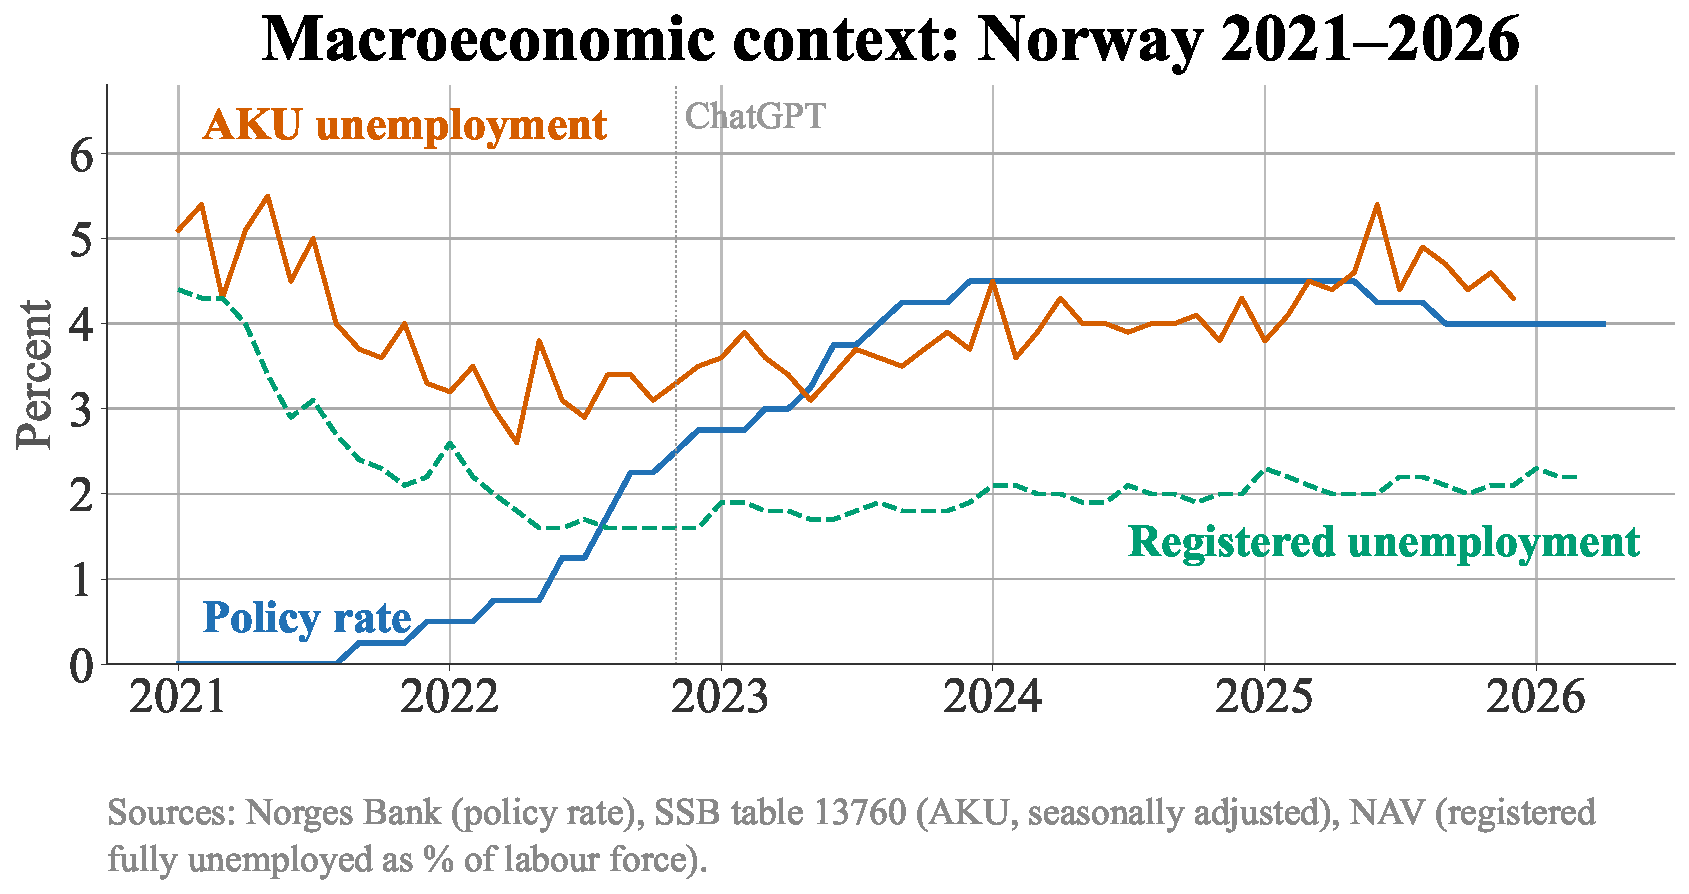
\includegraphics[width=0.8\textwidth]{../analysis/output/figures/figureA0a_macro_context.pdf}
  \caption{Macroeconomic context: Norges Bank policy rate and registered unemployment rate, 2021--2026.}
  \label{fig:macro_context}
\end{figure}

\begin{figure}[htbp]
  \centering
  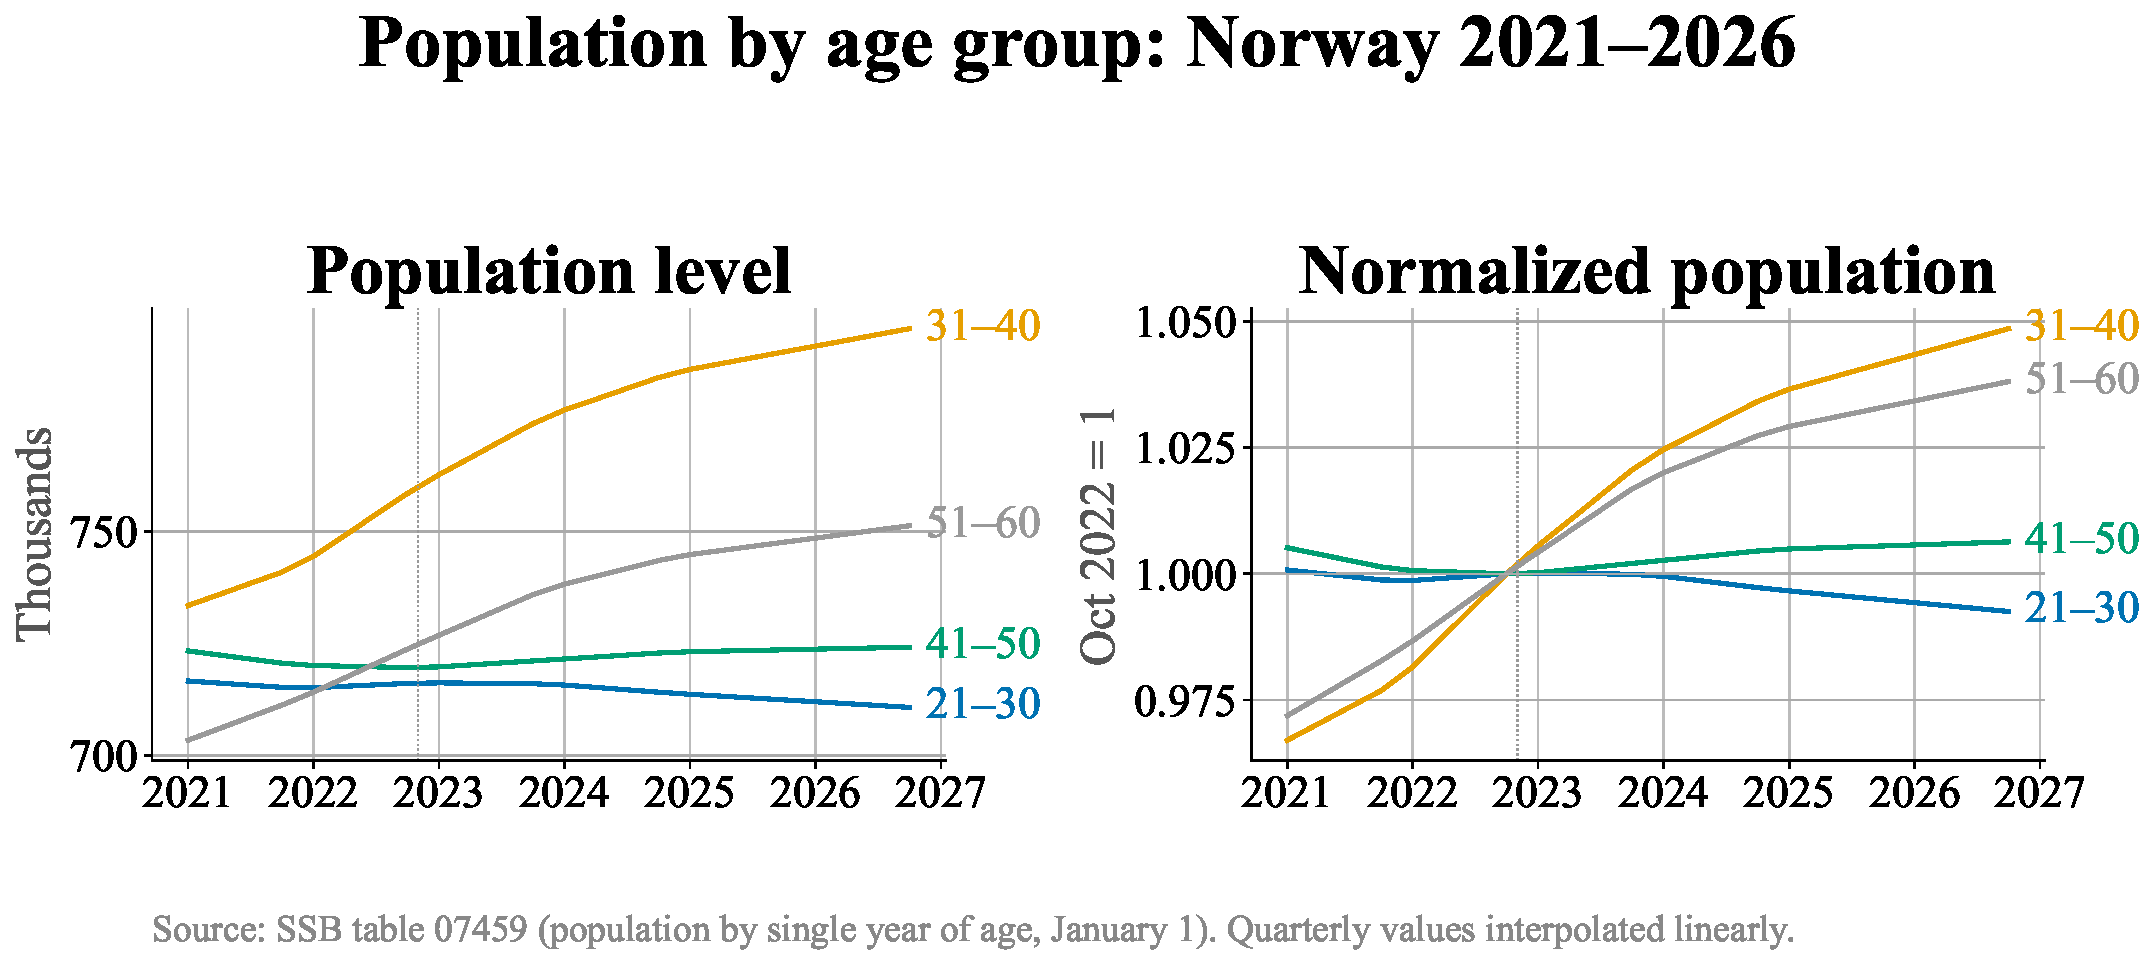
\includegraphics[width=0.8\textwidth]{../analysis/output/figures/figureA0b_cohort_sizes.pdf}
  \caption{Resident population by decade age group, 2021--2026.}
  \label{fig:cohort_sizes}
\end{figure}

\begin{figure}[htbp]
  \centering
  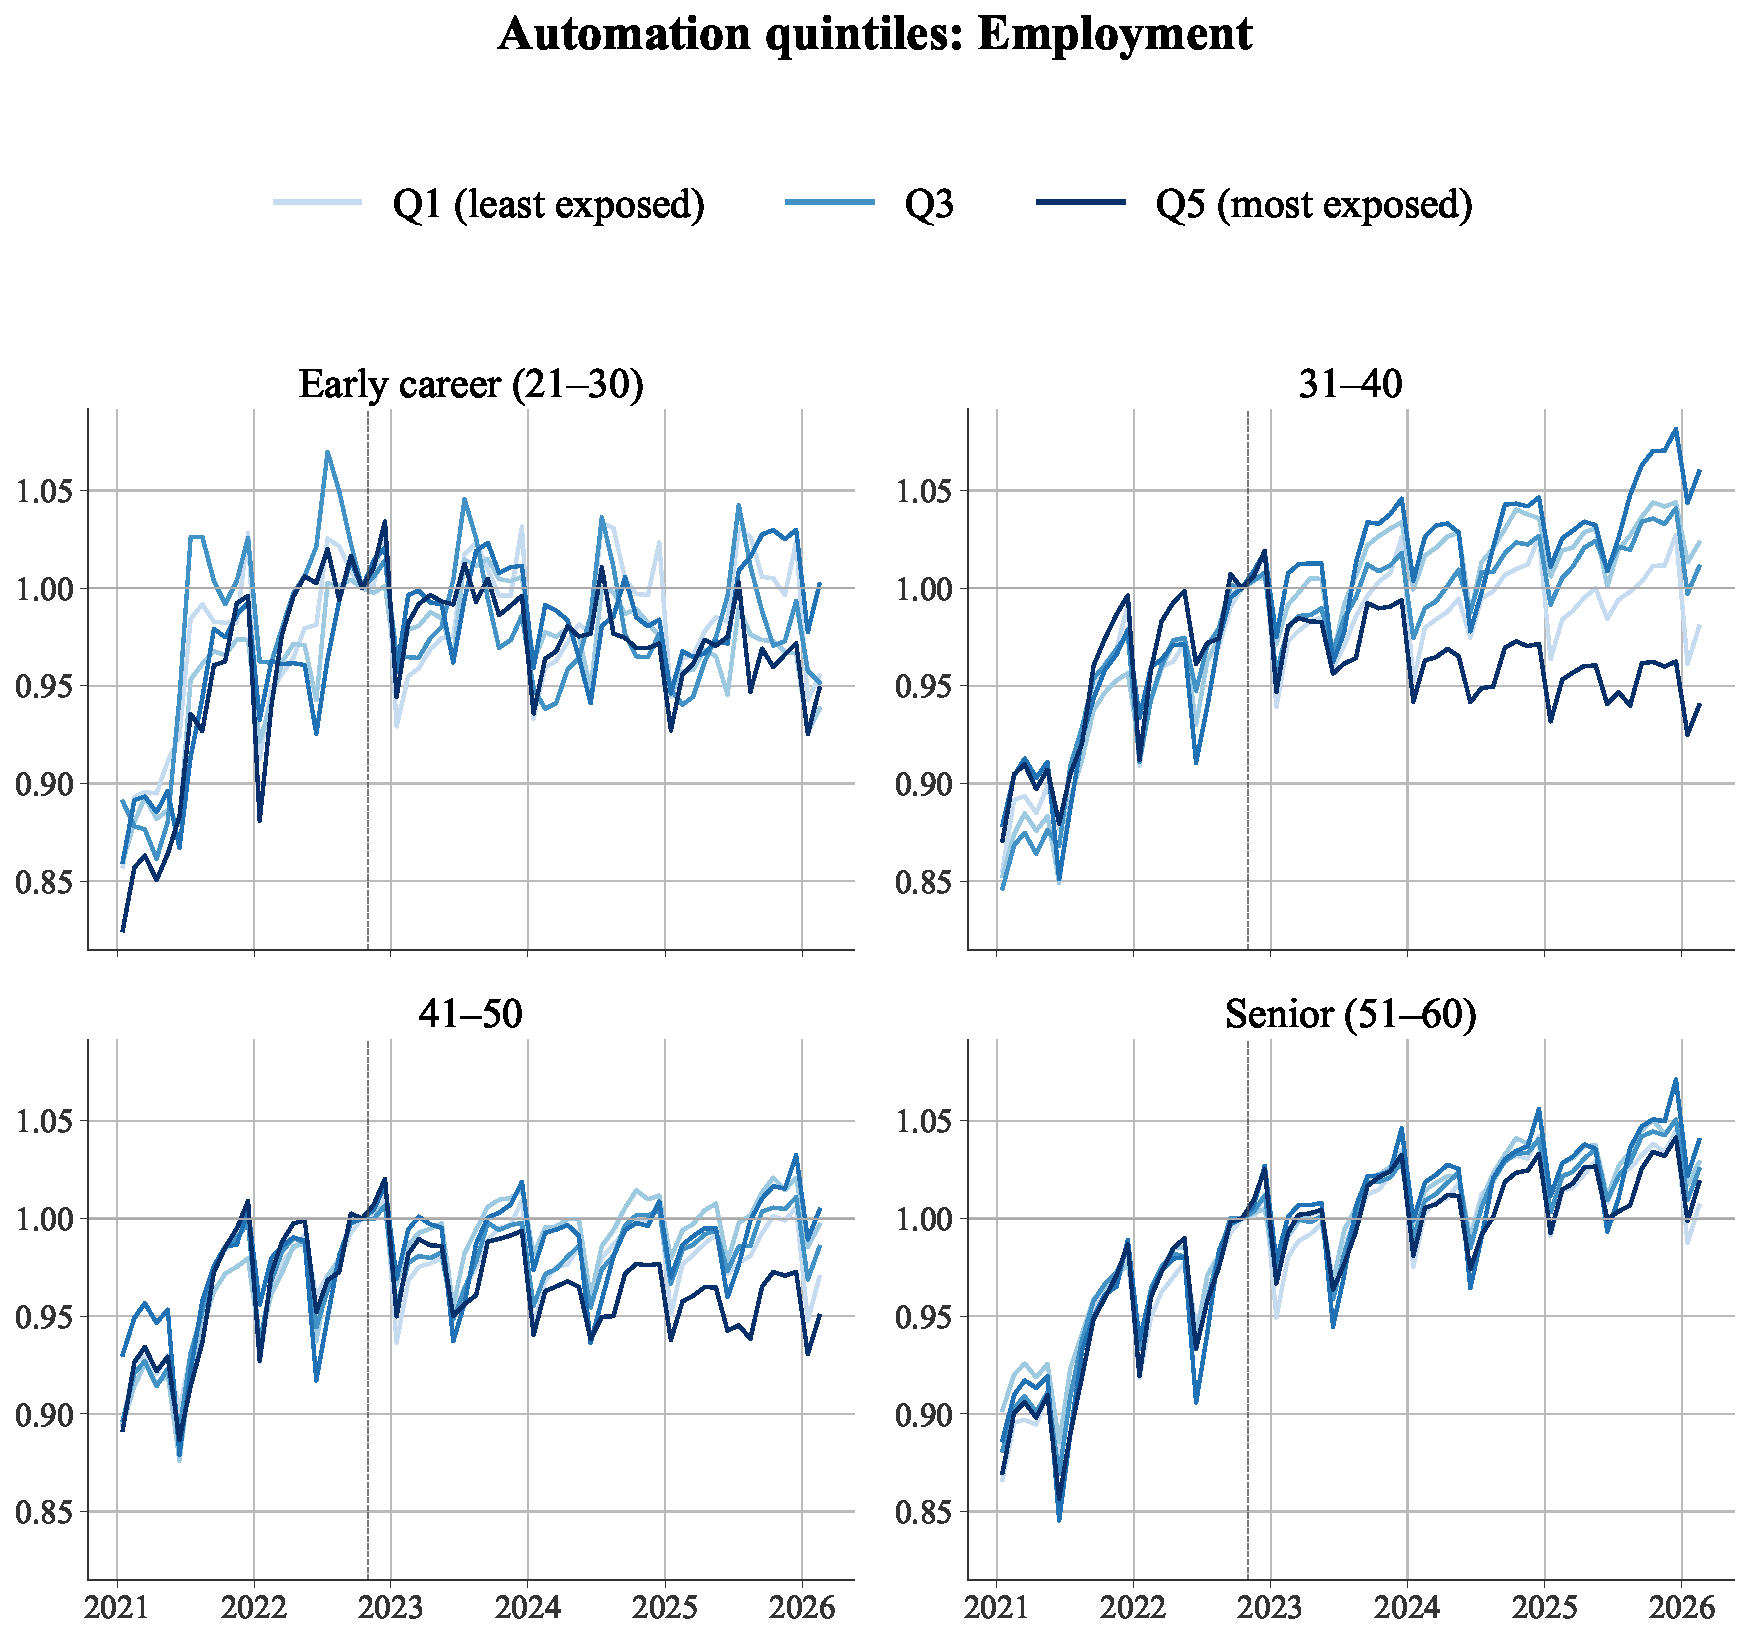
\includegraphics[width=\textwidth]{../analysis/output/figures/figure5b_age_by_quintile_handa.pdf}
  \caption{Employment by Handa et al.\ automation-exposure quintile and decade age group, private sector.}
  \label{fig:age_by_quintile_handa_auto}
  \begin{minipage}{\textwidth}\footnotesize\textit{Notes:} Private-sector employment indexed to October 2022 = 1. Occupations are ranked by the Handa et al.\ automation share.\end{minipage}
\end{figure}

\begin{figure}[htbp]
  \centering
  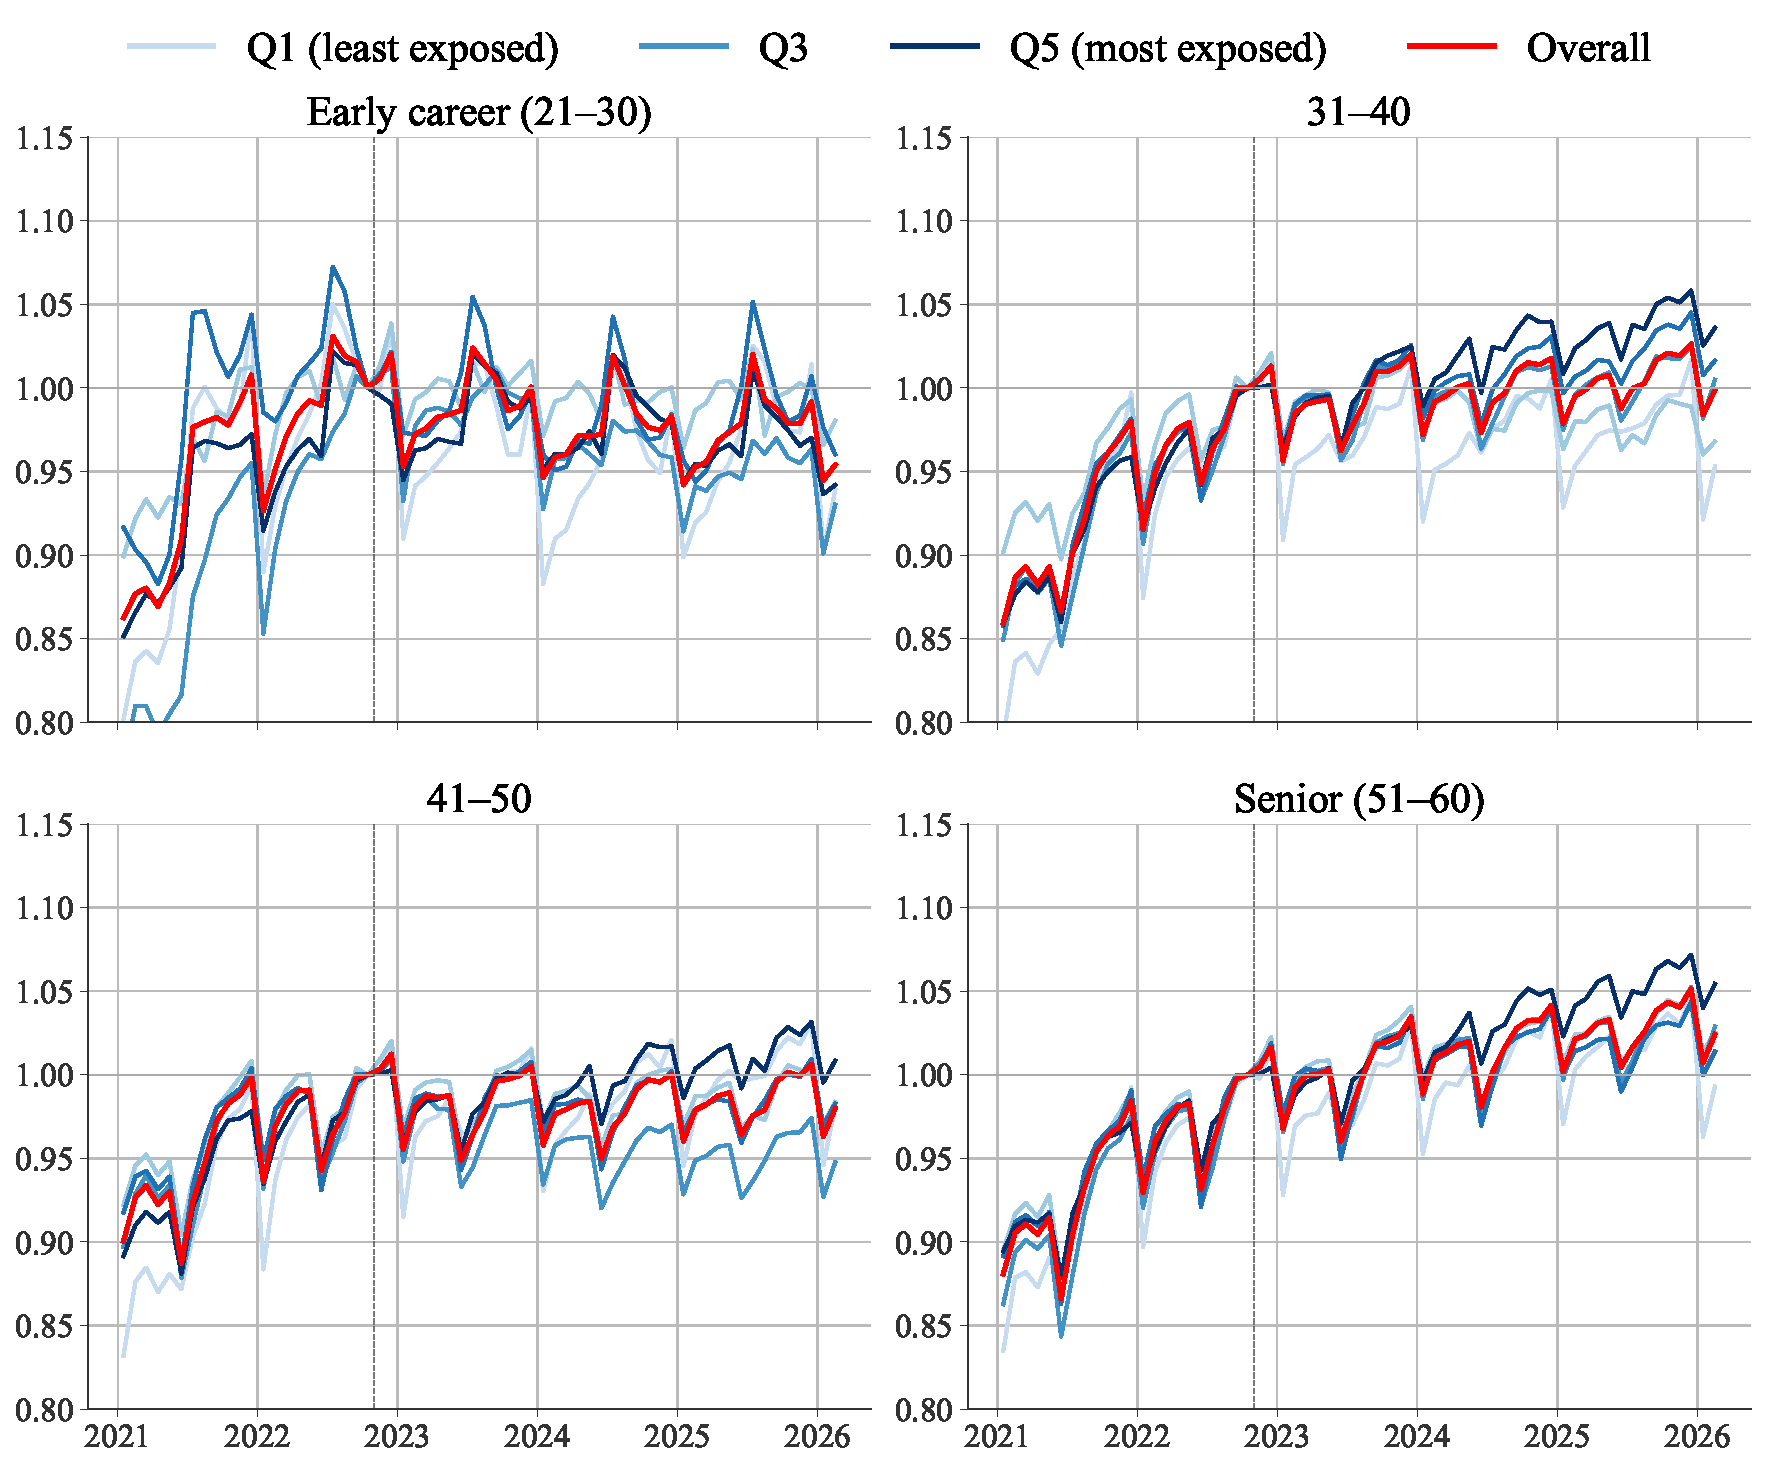
\includegraphics[width=\textwidth]{../analysis/output/figures/figure5c_age_by_quintile_handa.pdf}
  \caption{Employment by Handa et al.\ augmentation-exposure quintile and decade age group, private sector.}
  \label{fig:age_by_quintile_handa_aug}
  \begin{minipage}{\textwidth}\footnotesize\textit{Notes:} Private-sector employment indexed to October 2022 = 1. Occupations are ranked by the Handa et al.\ augmentation share.\end{minipage}
\end{figure}

\begin{figure}[htbp]
  \centering
  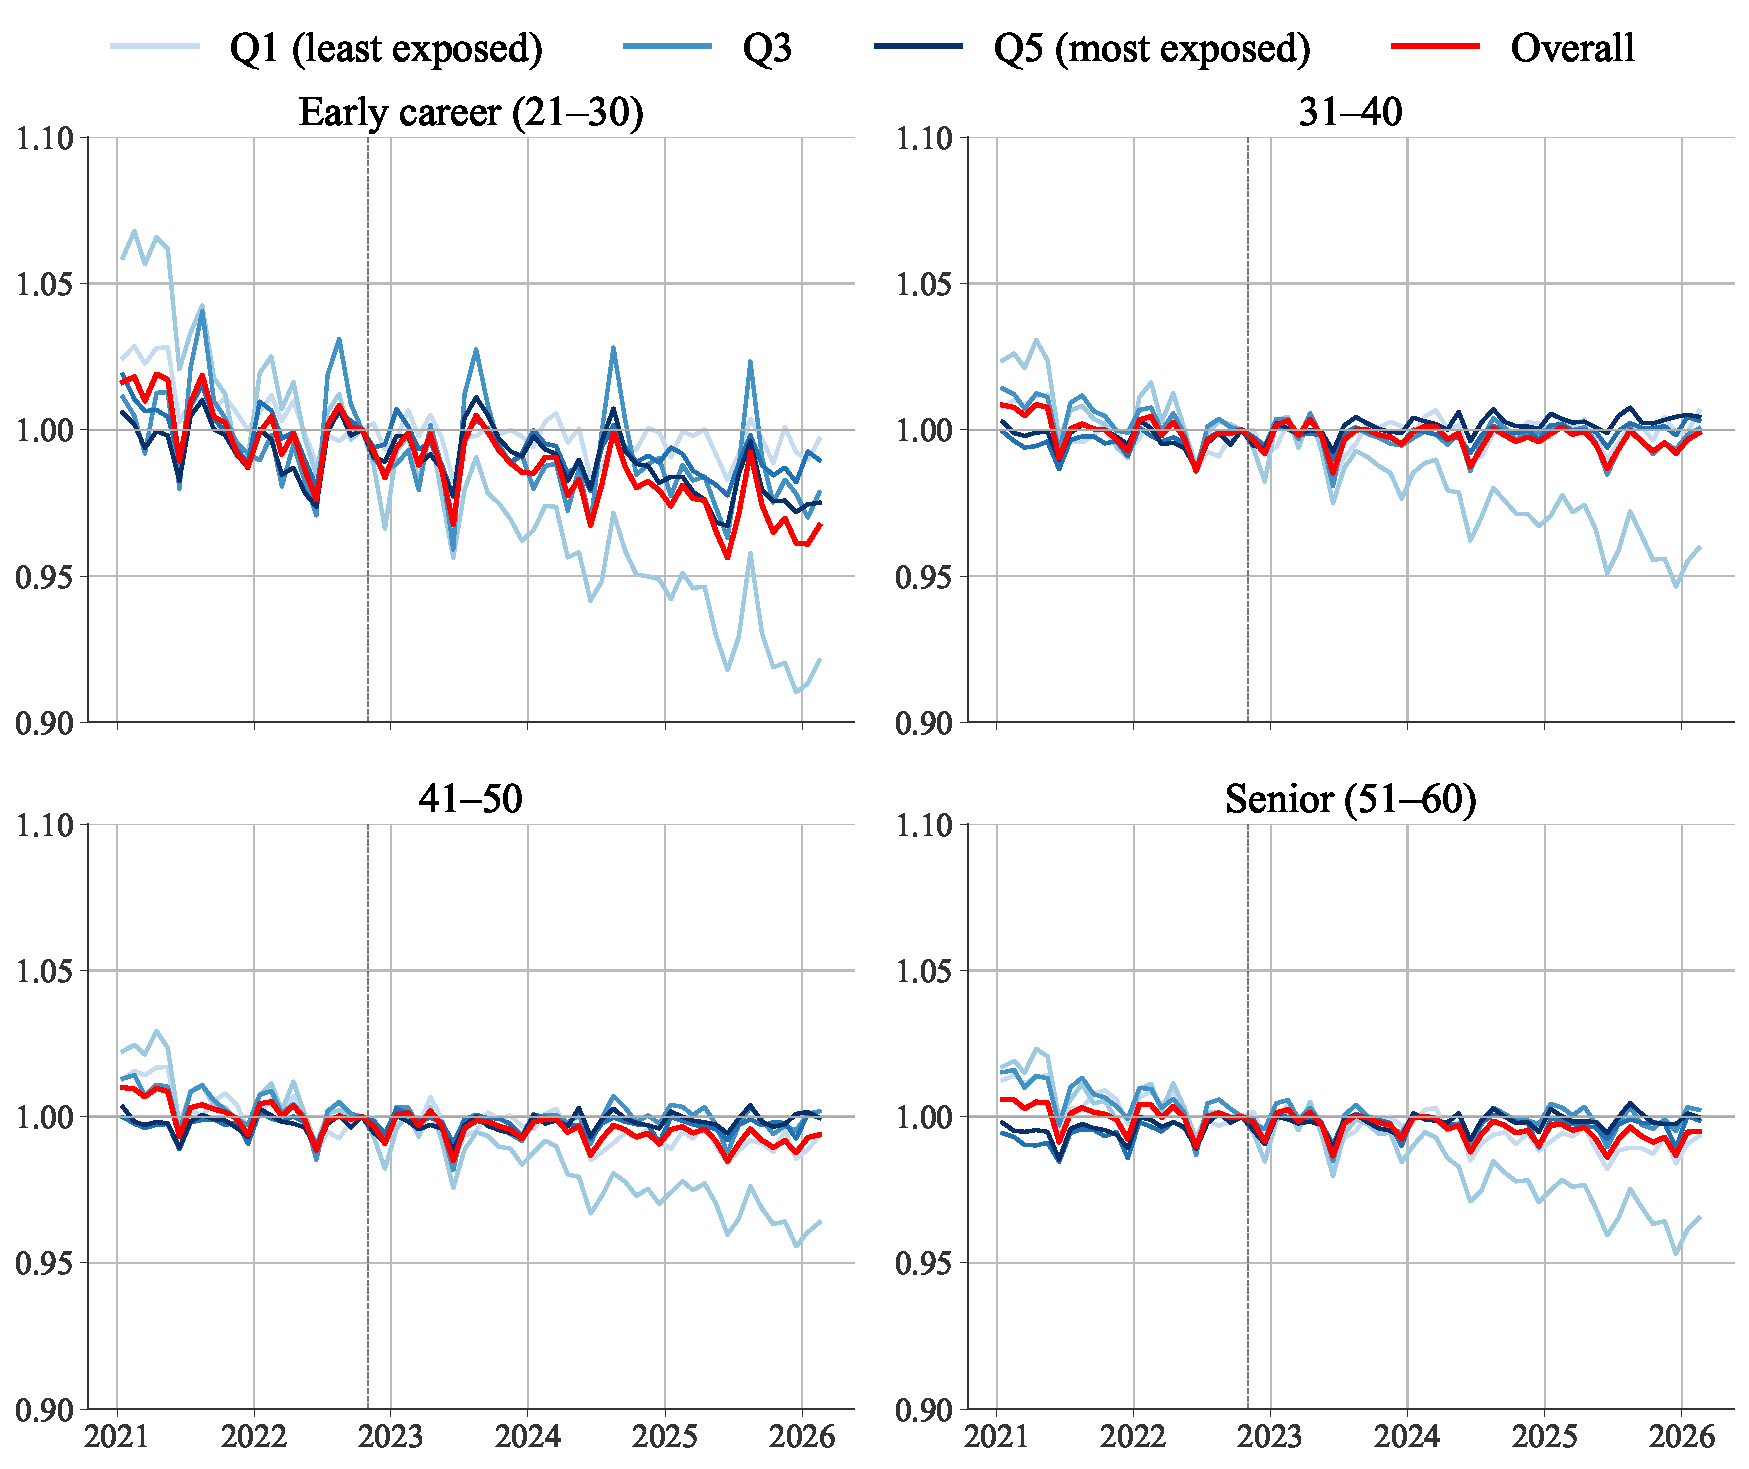
\includegraphics[width=\textwidth]{../analysis/output/figures/figure_stillingspst_decade_private.pdf}
  \caption{Position percentage by AI-exposure quintile and decade age group, private sector.}
  \label{fig:stillingspst_by_quintile}
  \begin{minipage}{\textwidth}\footnotesize\textit{Notes:} Mean contracted position percentage, indexed to October 2022 = 1. Occupations are ranked by the Eloundou et al.\ exposure score.\end{minipage}
\end{figure}

\begin{figure}[htbp]
  \centering
  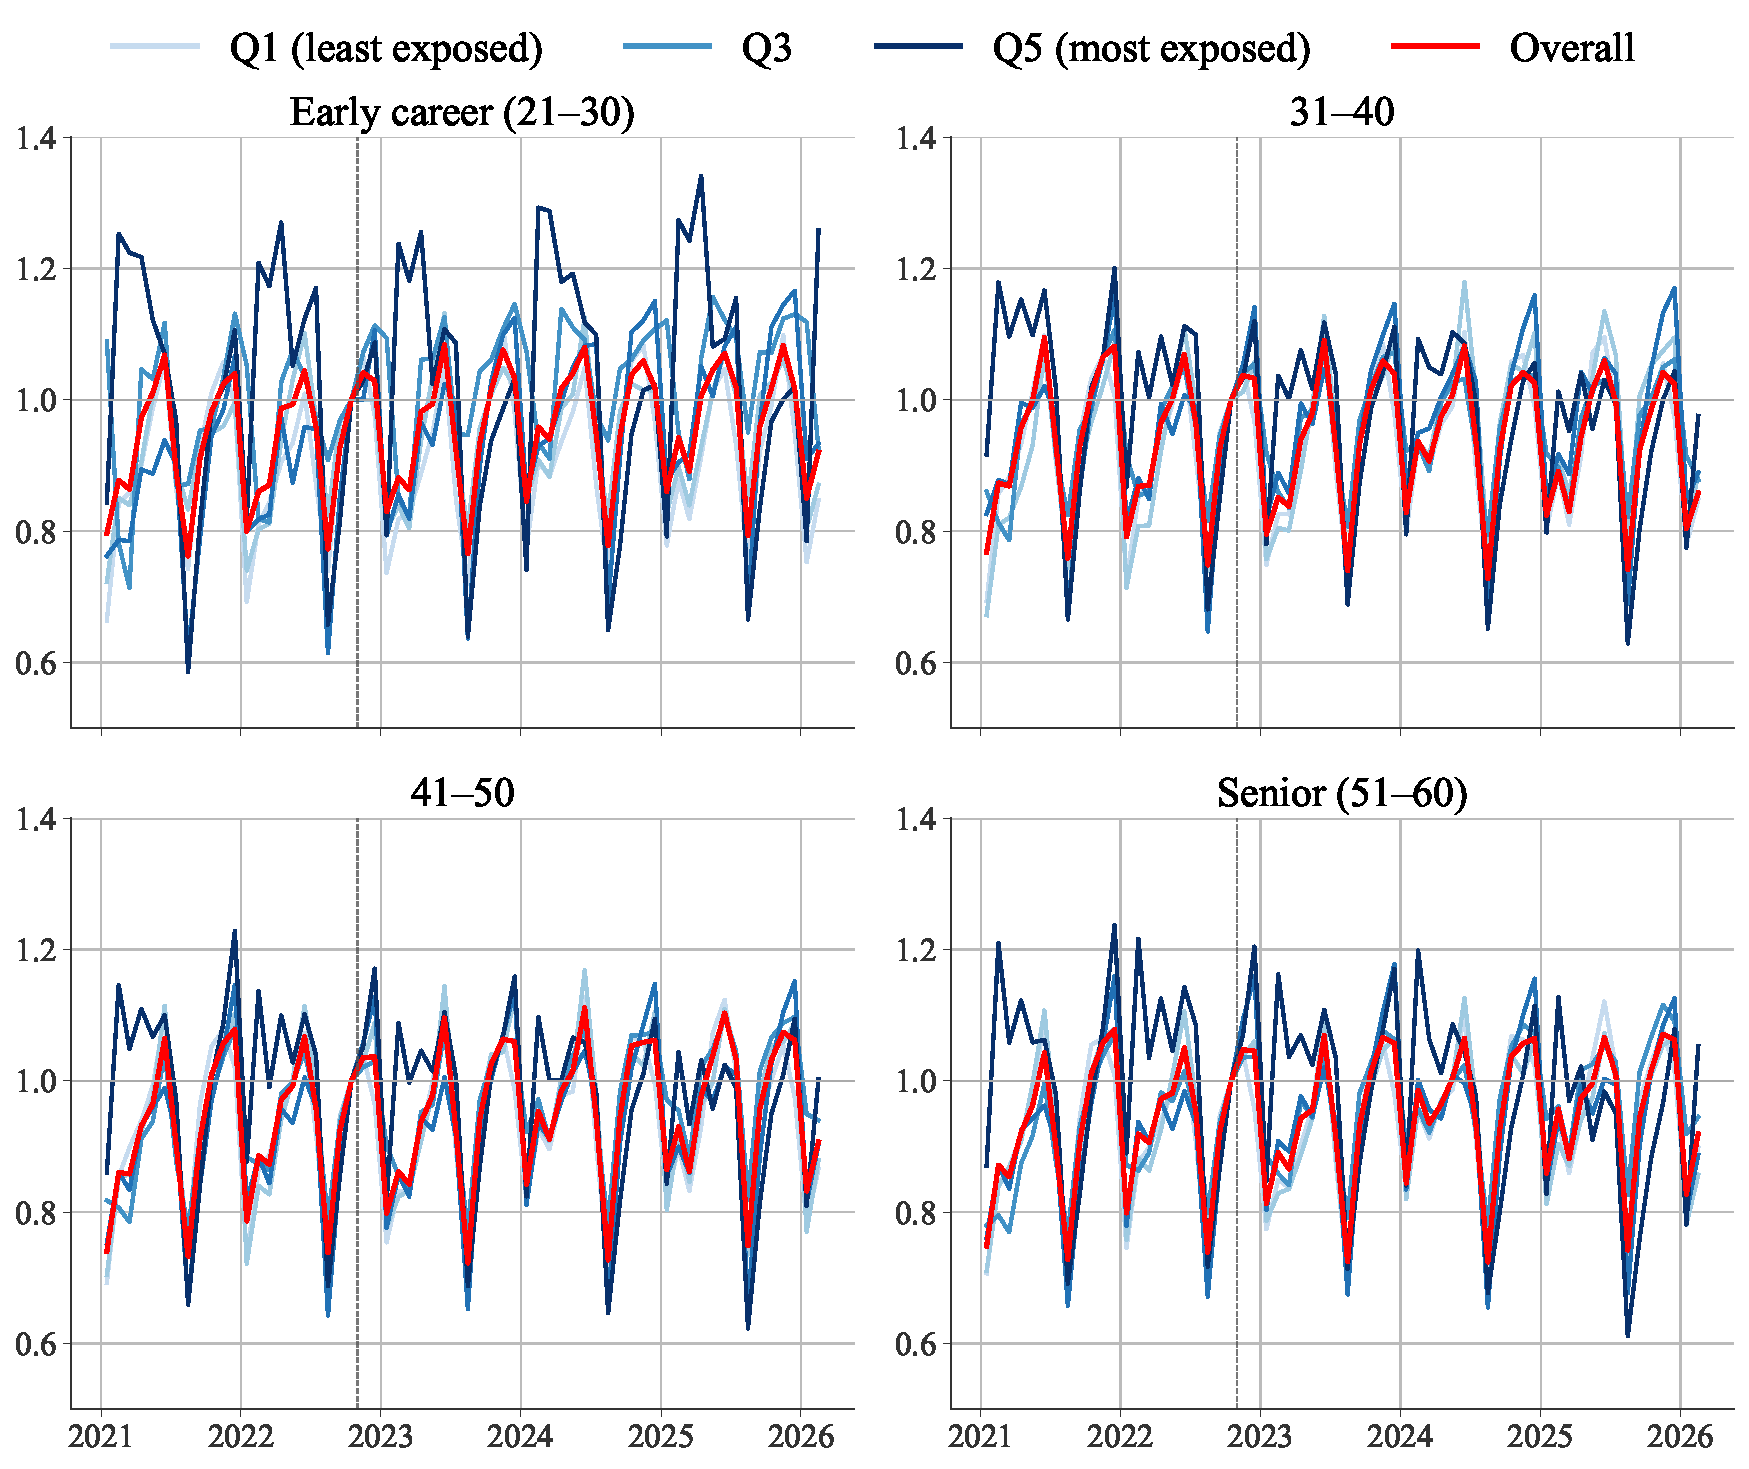
\includegraphics[width=\textwidth]{../analysis/output/figures/figure_overtid_timer_decade_private.pdf}
  \caption{Overtime hours by AI-exposure quintile and decade age group, private sector.}
  \label{fig:overtid_by_quintile}
  \begin{minipage}{\textwidth}\footnotesize\textit{Notes:} Mean overtime hours, indexed to October 2022 = 1. Occupations are ranked by the Eloundou et al.\ exposure score.\end{minipage}
\end{figure}

\begin{figure}[htbp]
  \centering
  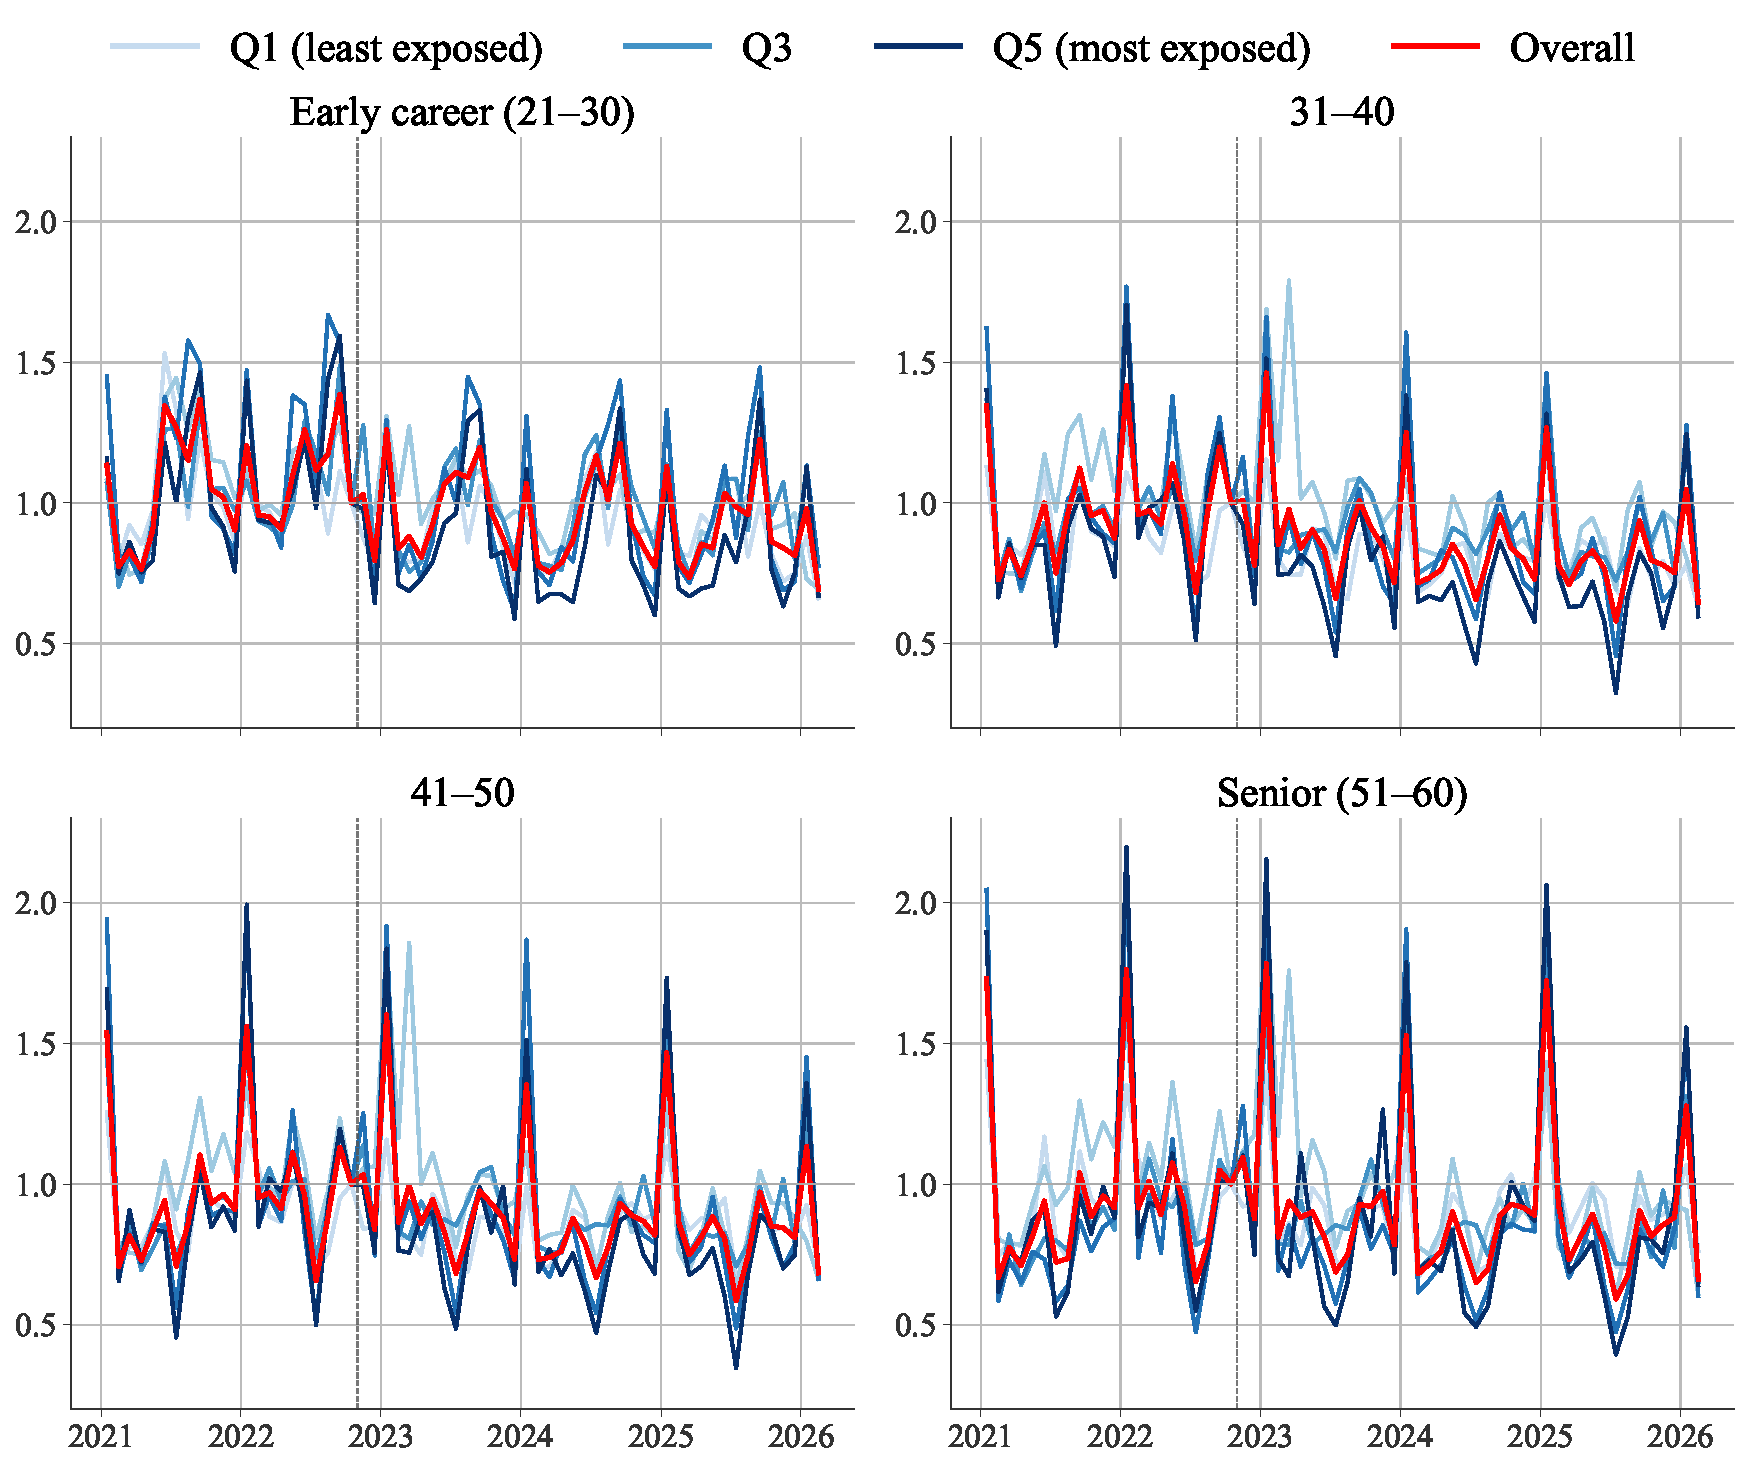
\includegraphics[width=\textwidth]{../analysis/output/figures/figure_ny_jobb_decade_private.pdf}
  \caption{New-hire share by AI-exposure quintile and decade age group, private sector.}
  \label{fig:nyjobb_by_quintile}
  \begin{minipage}{\textwidth}\footnotesize\textit{Notes:} Mean new-hire share, indexed to October 2022 = 1. Occupations are ranked by the Eloundou et al.\ exposure score.\end{minipage}
\end{figure}

\begin{figure}[htbp]
  \centering
  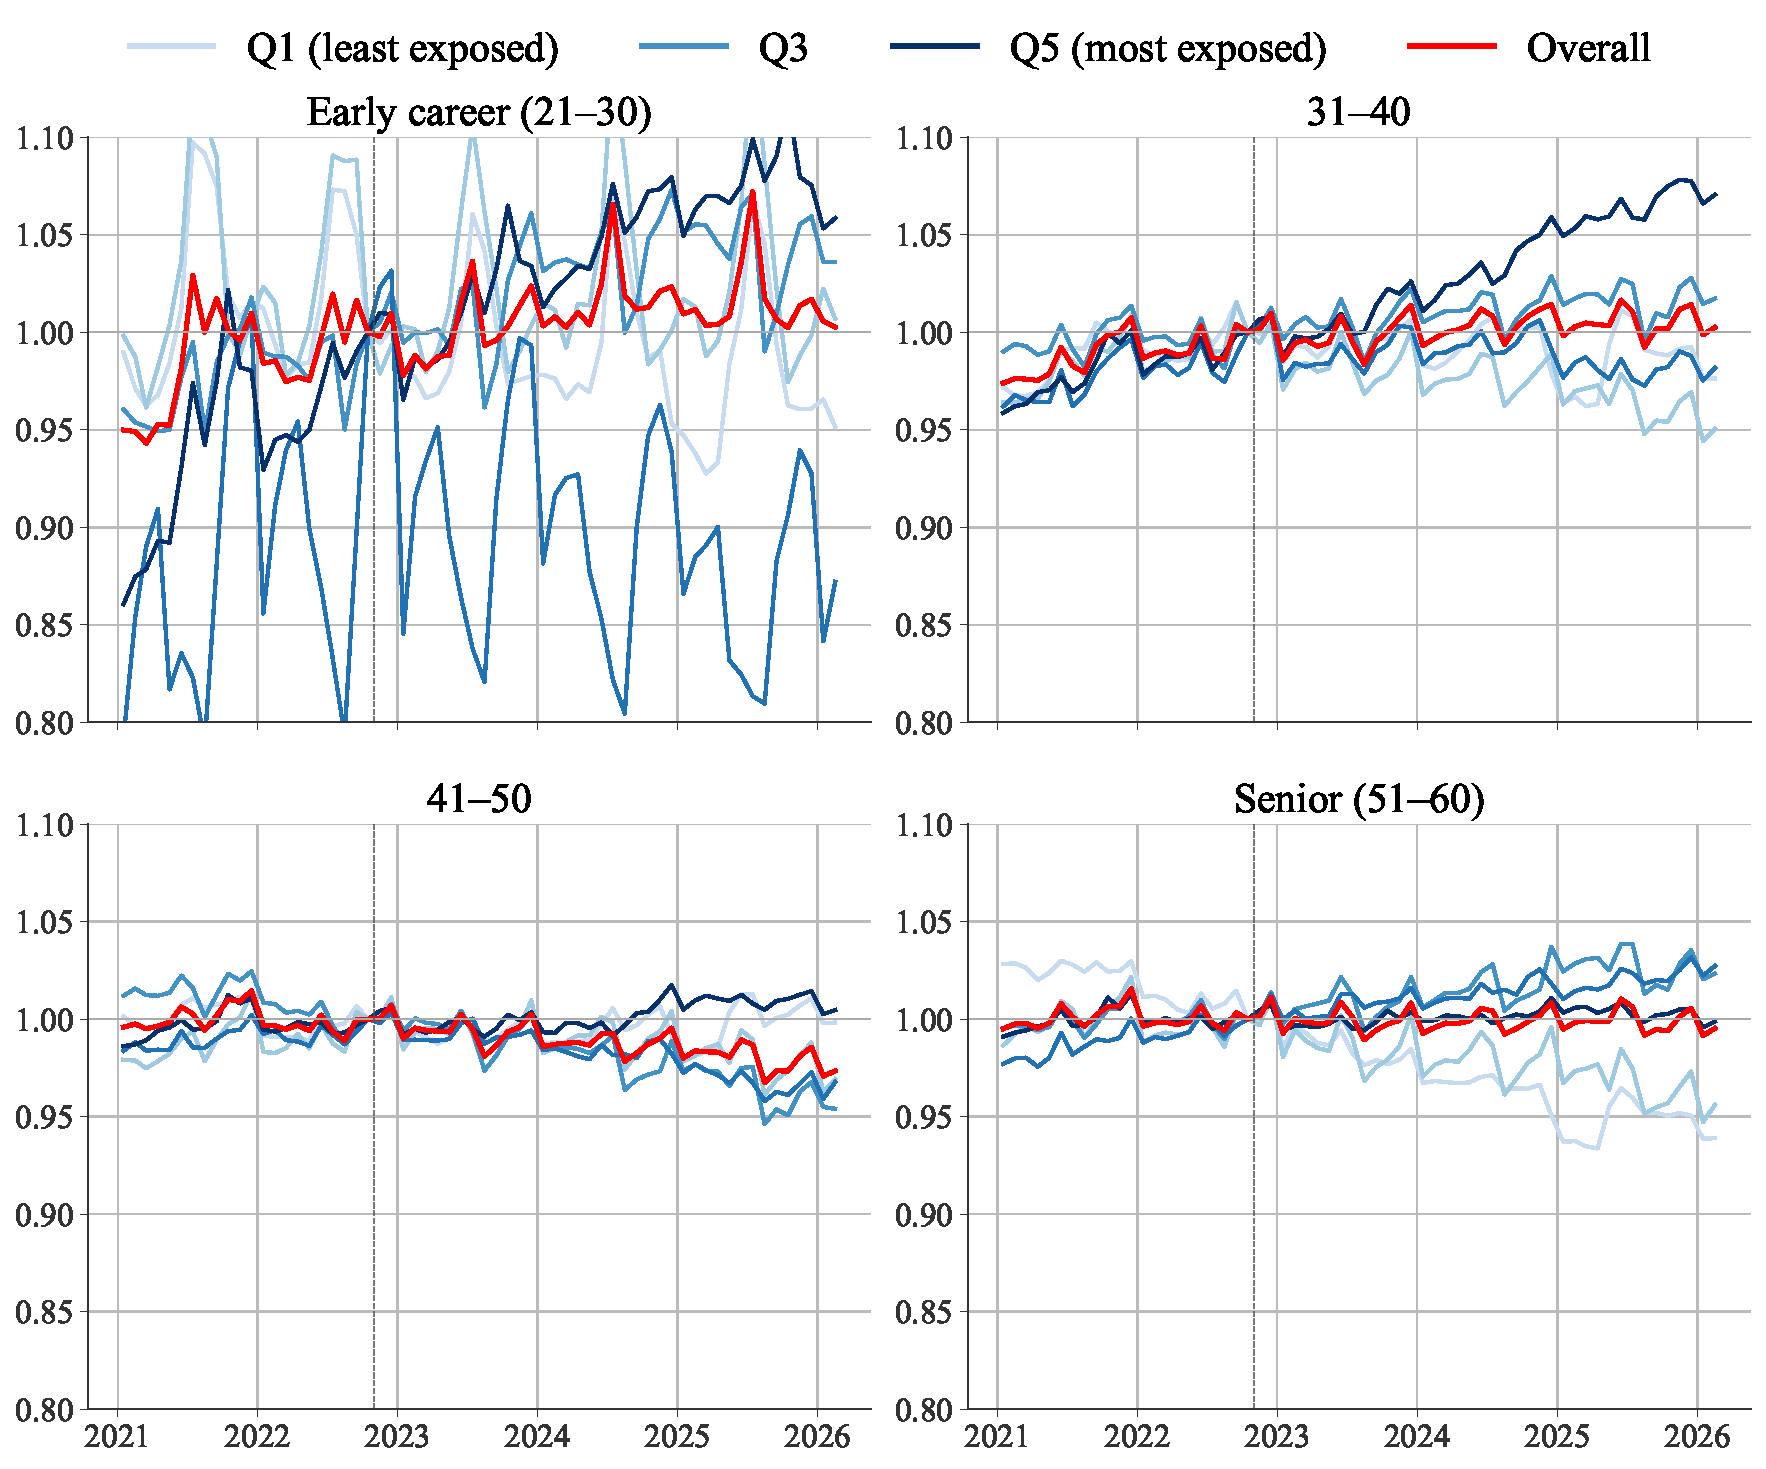
\includegraphics[width=\textwidth]{../analysis/output/figures/figure_emp_decade_public.pdf}
  \caption{Employment by AI-exposure quintile and decade age group, public sector.}
  \label{fig:emp_public}
  \begin{minipage}{\textwidth}\footnotesize\textit{Notes:} Public-sector employment per capita, indexed to October 2022 = 1. Occupations are ranked by the Eloundou et al.\ exposure score. Q1 (lightest) = least exposed; Q5 (darkest) = most exposed. Red line = overall age-group trend. Vertical dashed line marks the November 2022 ChatGPT release.\end{minipage}
\end{figure}

\begin{figure}[htbp]
  \centering
  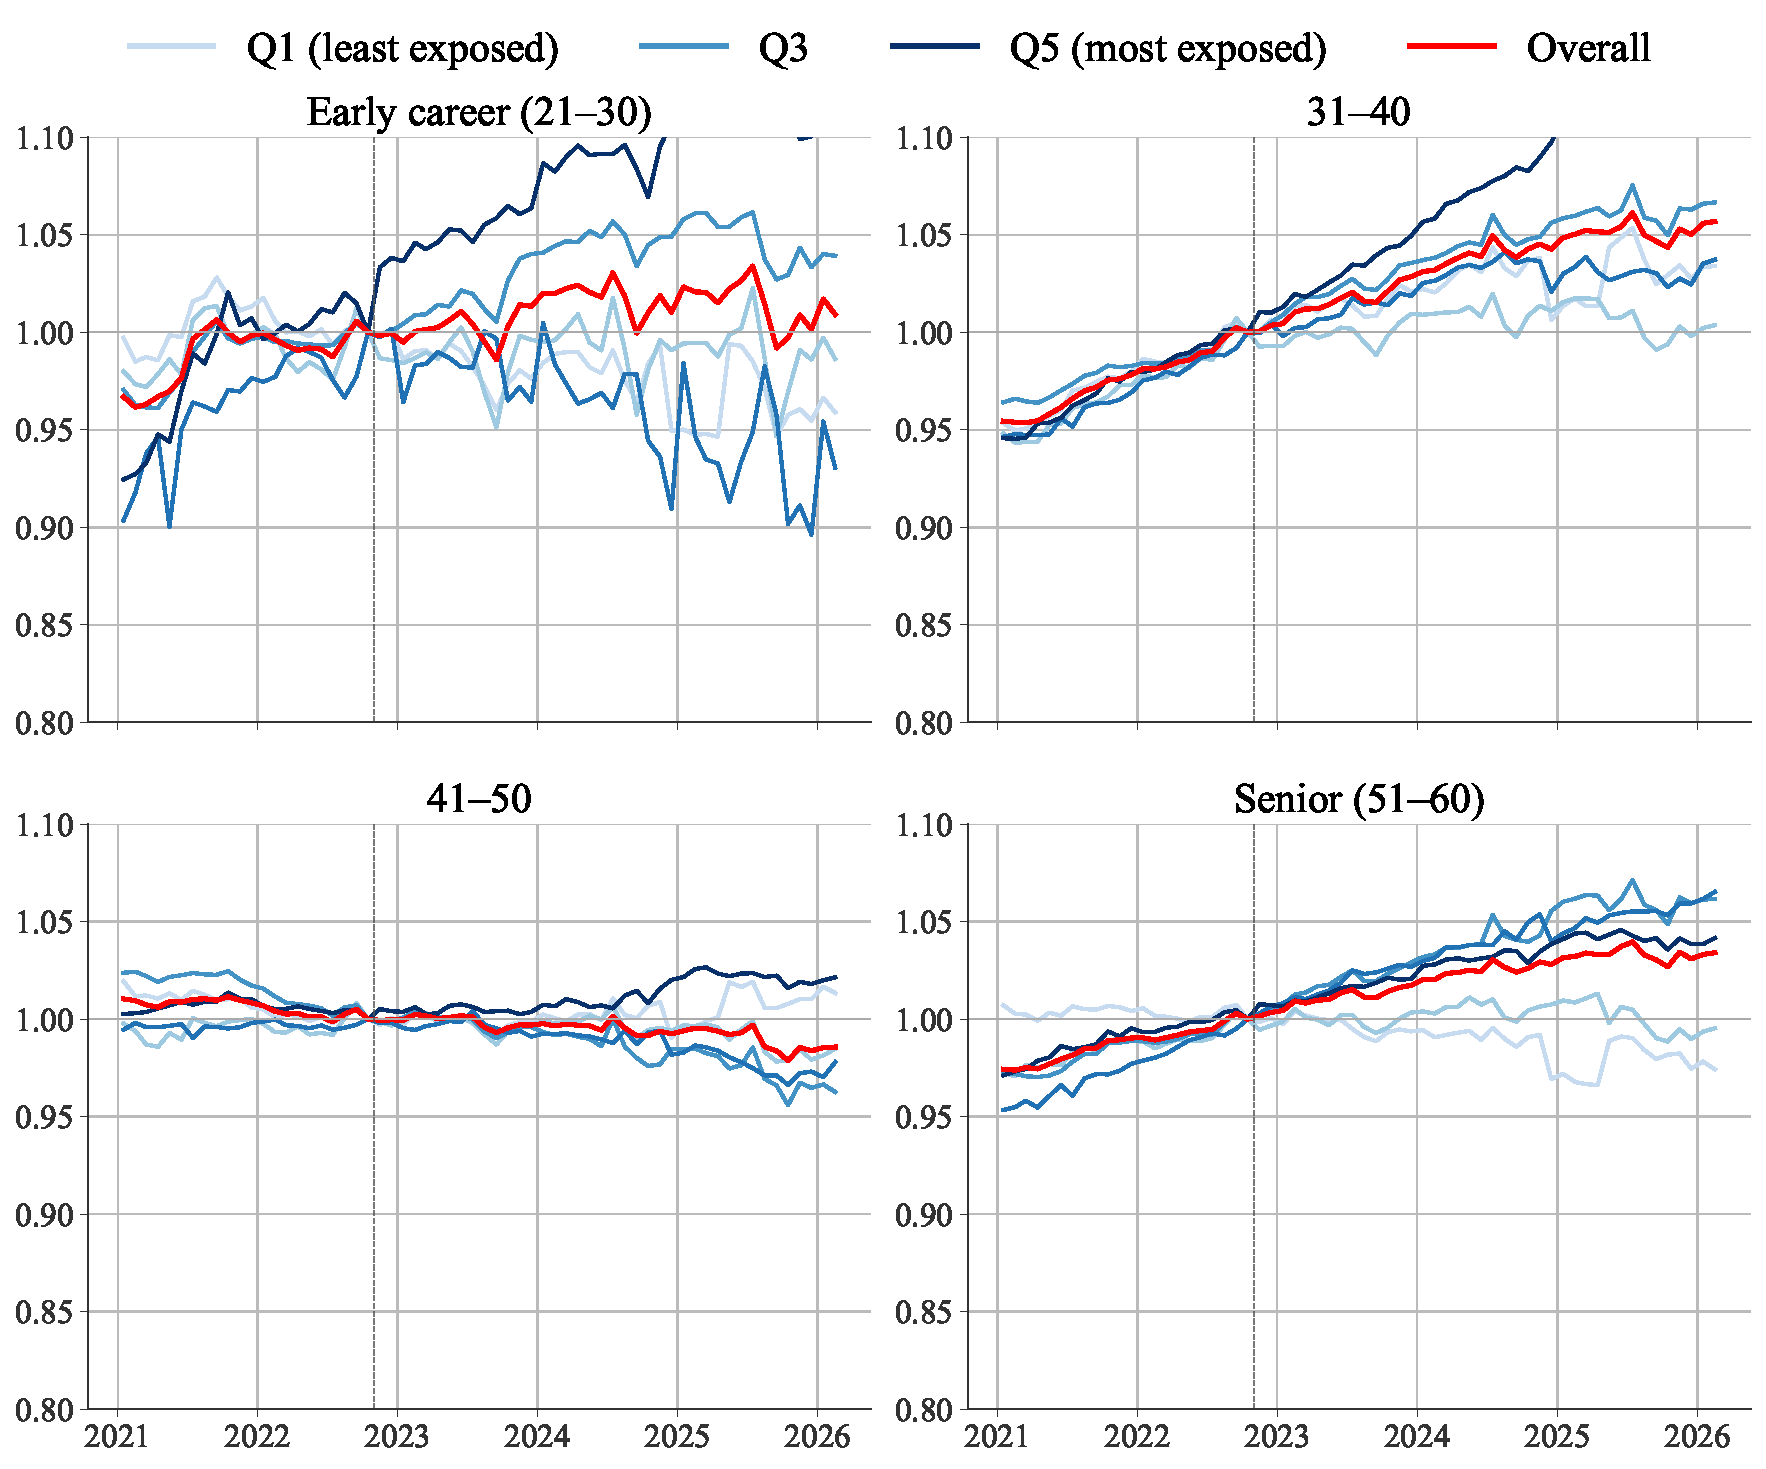
\includegraphics[width=\textwidth]{../analysis/output/figures/figure_emp_decade_public_sa.pdf}
  \caption{Employment by AI-exposure quintile and decade age group, public sector, seasonally adjusted.}
  \label{fig:emp_public_sa}
  \begin{minipage}{\textwidth}\footnotesize\textit{Notes:} Seasonally adjusted counterpart of Figure~\ref{fig:emp_public}; public-sector headcount, frozen X-11 adjustment (factors estimated 2021--2024), indexed to October 2022 = 1. Q1 (lightest) = least exposed; Q5 (darkest) = most exposed.\end{minipage}
\end{figure}


% =============================================================================
\clearpage
\phantomsection
\addcontentsline{toc}{section}{Appendix B: Brynjolfsson et al.\ Replication}
\section*{Appendix B: Brynjolfsson et al.\ Replication}\label{app:bcc}
\setcounter{figure}{0}
\renewcommand{\thefigure}{B\arabic{figure}}

We replicate the design of \citet{brynjolfsson2025} on Norwegian register data, on the exact early-career definition used in the cross-country literature. The sample is full-time private-sector workers in foretak with at least 10 workers in each age group every month and at least 100 worker-months per firm-quintile-age cell, the balanced-panel construction used in their paper. Workers are placed in six age bins (22--25, 26--30, 31--34, 35--40, 41--49, 50--55) that match their 22--25 early-career definition, employment is indexed to October 2022, and occupations are ranked by the Eloundou GPT-4 quintile. This sample is smaller and more concentrated in larger firms than the main analysis, so its raw series move more than the population series in the main text.

Figure~\ref{fig:bcc_es} reports the Poisson event study. For workers aged 22--25 the post-October-2022 average gap is small, about 3 log points, but it masks a clear time profile: the most-exposed and least-exposed quintiles track each other through early 2025, and from spring 2025 the most-exposed quintile falls below, with the gap widening to about 35 log points by February 2026. This widening rests on the final ten months of data, the confidence intervals are wide, and the joint pre-trend test rejects parallel trends, so it is an emerging pattern rather than an identified effect. The recent gap exceeds the 15 log points \citet{brynjolfsson2025} report for the United States, but the US gap opened earlier and over a far larger sample. The descriptive series behind the replication appear in Figures~\ref{fig:bcc_occ}--\ref{fig:bcc_comp}: selected occupations, the Eloundou exposure quintiles, the Handa usage split, and cash earnings.

\begin{figure}[htbp]
  \centering
  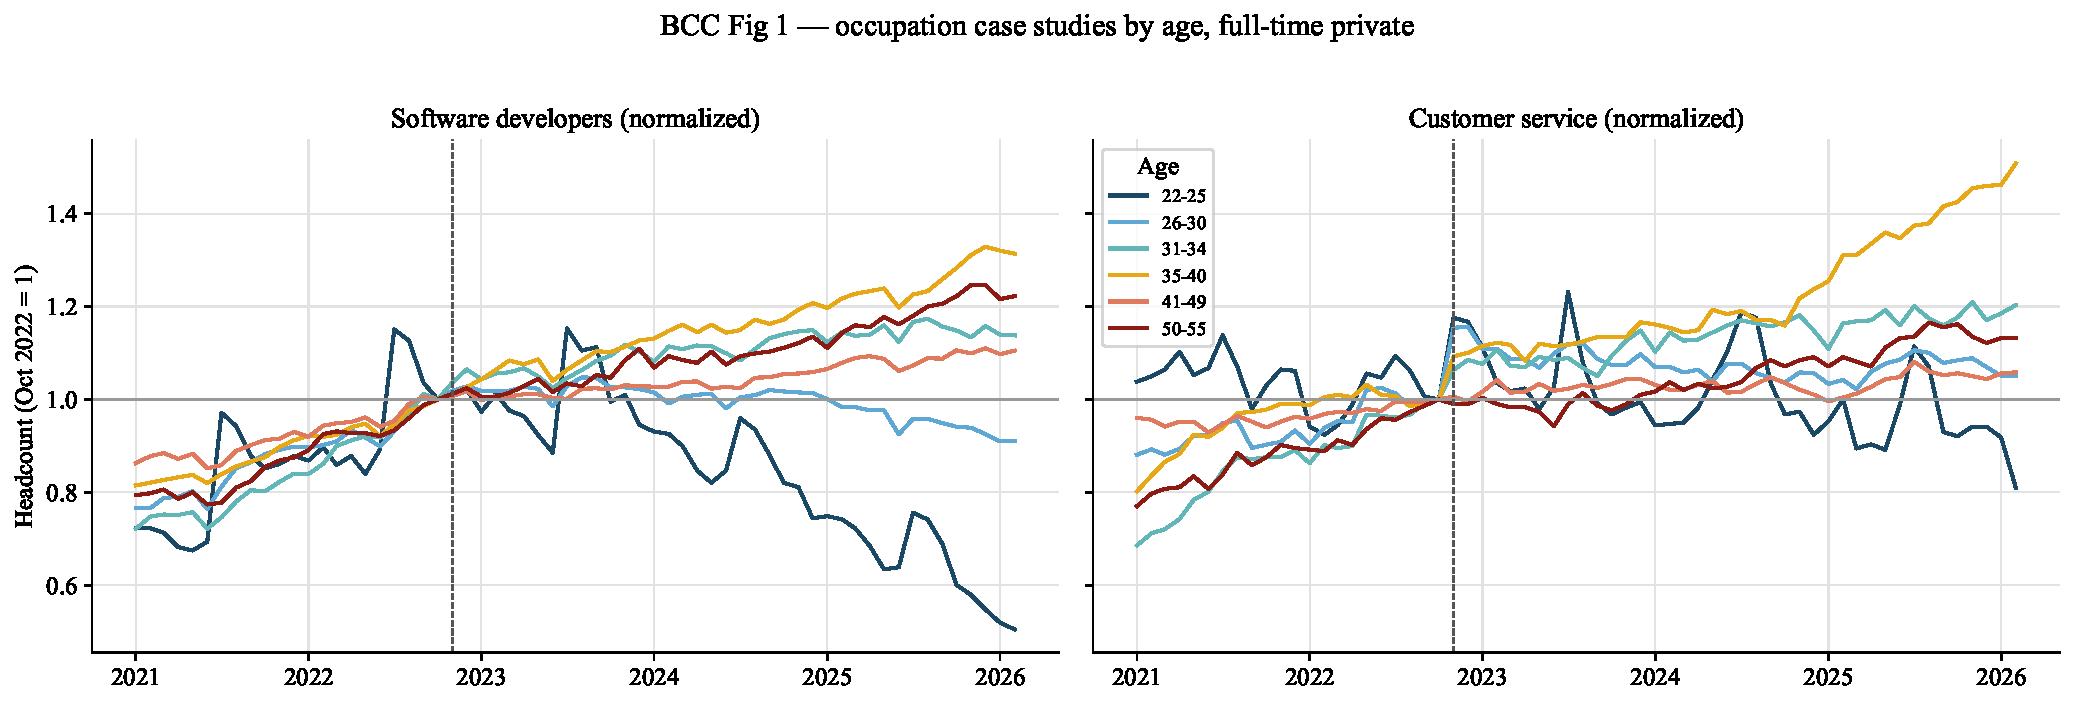
\includegraphics[width=\textwidth]{../analysis-indiv/output/bcc_appendix/fig_bcc_1_occ.pdf}
  \caption{Employment in selected occupations by age group, Brynjolfsson et al.\ replication.}
  \label{fig:bcc_occ}
  \begin{minipage}{\textwidth}\footnotesize\textit{Notes:} Employment indexed to October 2022 = 1, by age group, for software developers (ISCO-08 2512) and customer service (4222). Full-time private-sector workers in the balanced panel.\end{minipage}
\end{figure}

\begin{figure}[htbp]
  \centering
  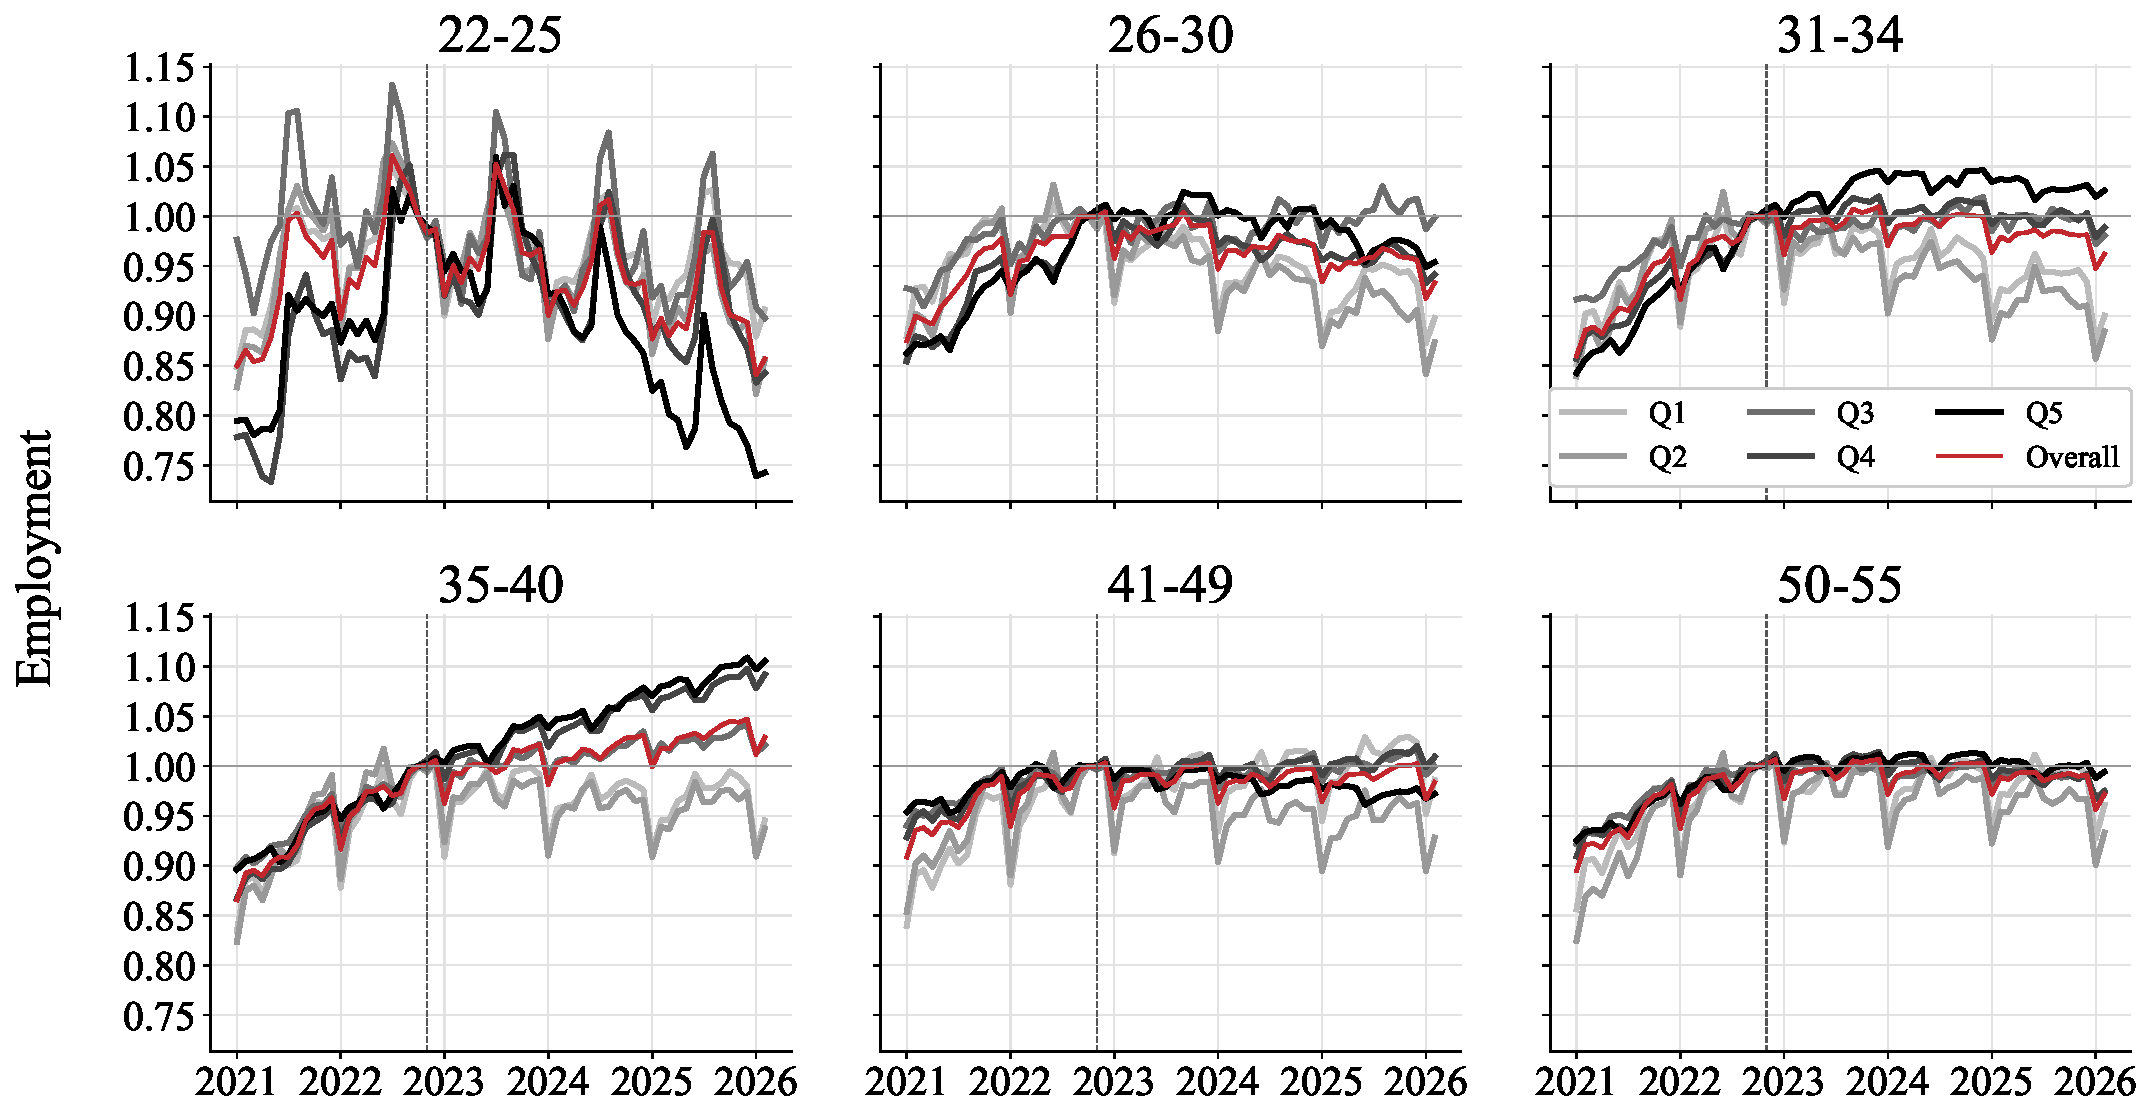
\includegraphics[width=\textwidth]{../analysis-indiv/output/bcc_appendix/fig_bcc_2_eloundou.pdf}
  \caption{Employment by Eloundou exposure quintile and age group, Brynjolfsson et al.\ replication.}
  \label{fig:bcc_eloundou}
  \begin{minipage}{\textwidth}\footnotesize\textit{Notes:} Employment indexed to October 2022 = 1, by Eloundou GPT-4 quintile within each age group, with a pooled overall line. Full-time private-sector workers in the balanced panel.\end{minipage}
\end{figure}

\begin{figure}[htbp]
  \centering
  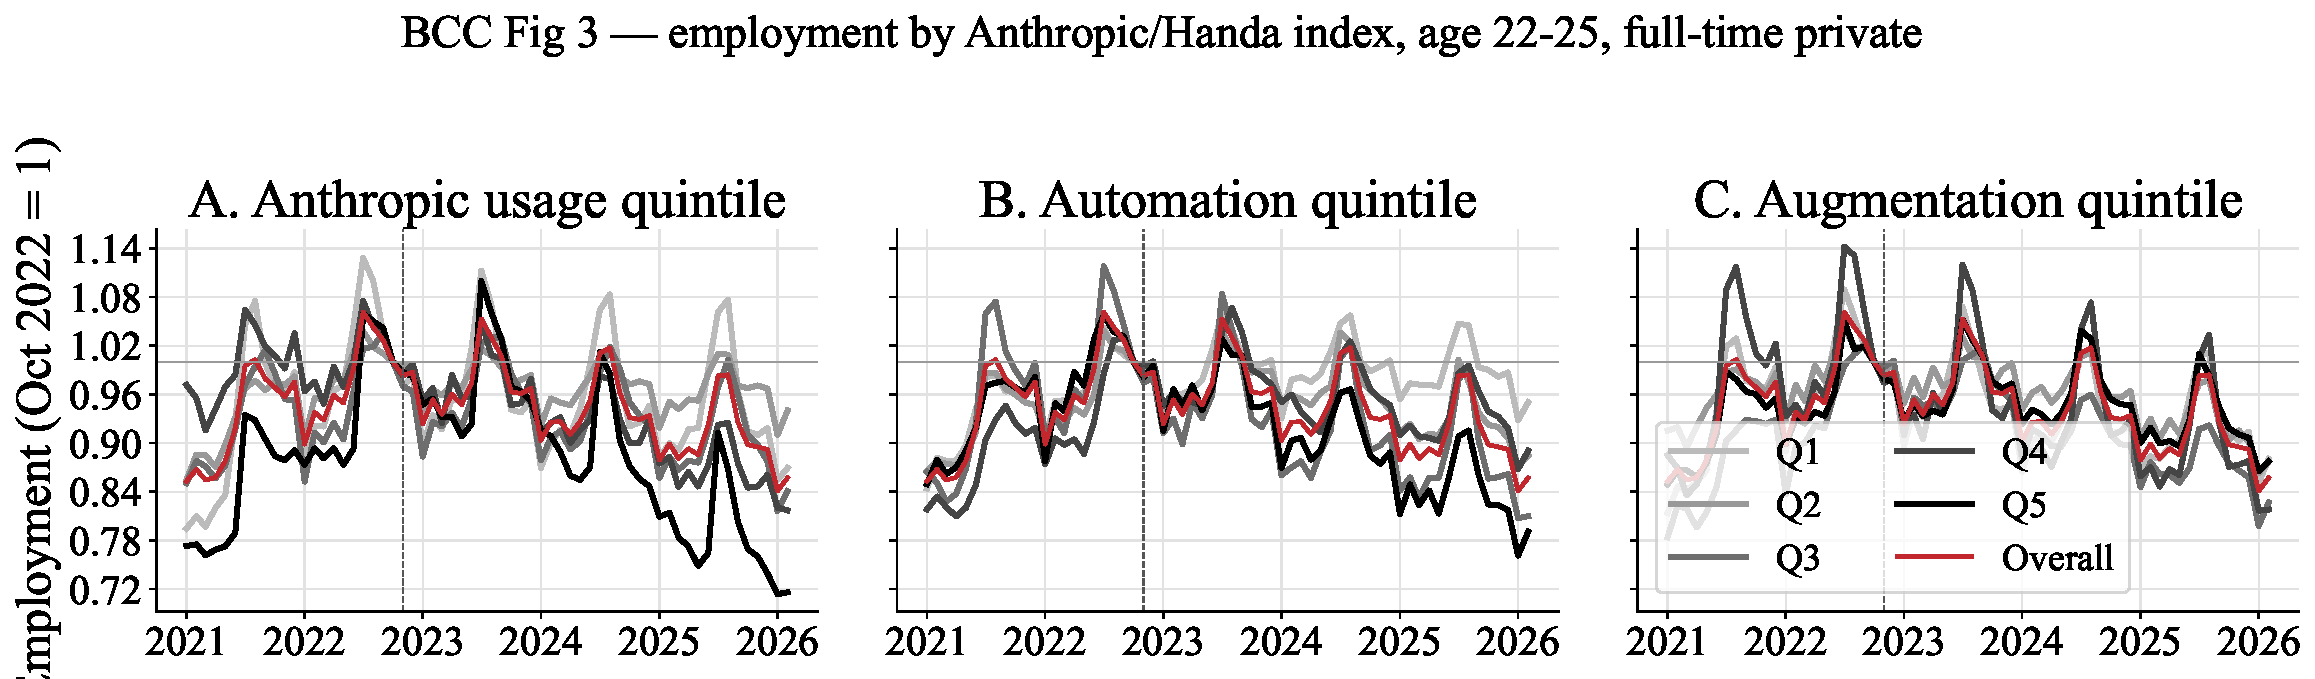
\includegraphics[width=\textwidth]{../analysis-indiv/output/bcc_appendix/fig_bcc_3_handa.pdf}
  \caption{Employment by Handa usage, automation, and augmentation quintile, ages 22--25.}
  \label{fig:bcc_handa}
  \begin{minipage}{\textwidth}\footnotesize\textit{Notes:} Employment indexed to October 2022 = 1 for workers aged 22--25, by Handa et al.\ usage, automation, and augmentation quintile, with a pooled overall line.\end{minipage}
\end{figure}

\begin{figure}[htbp]
  \centering
  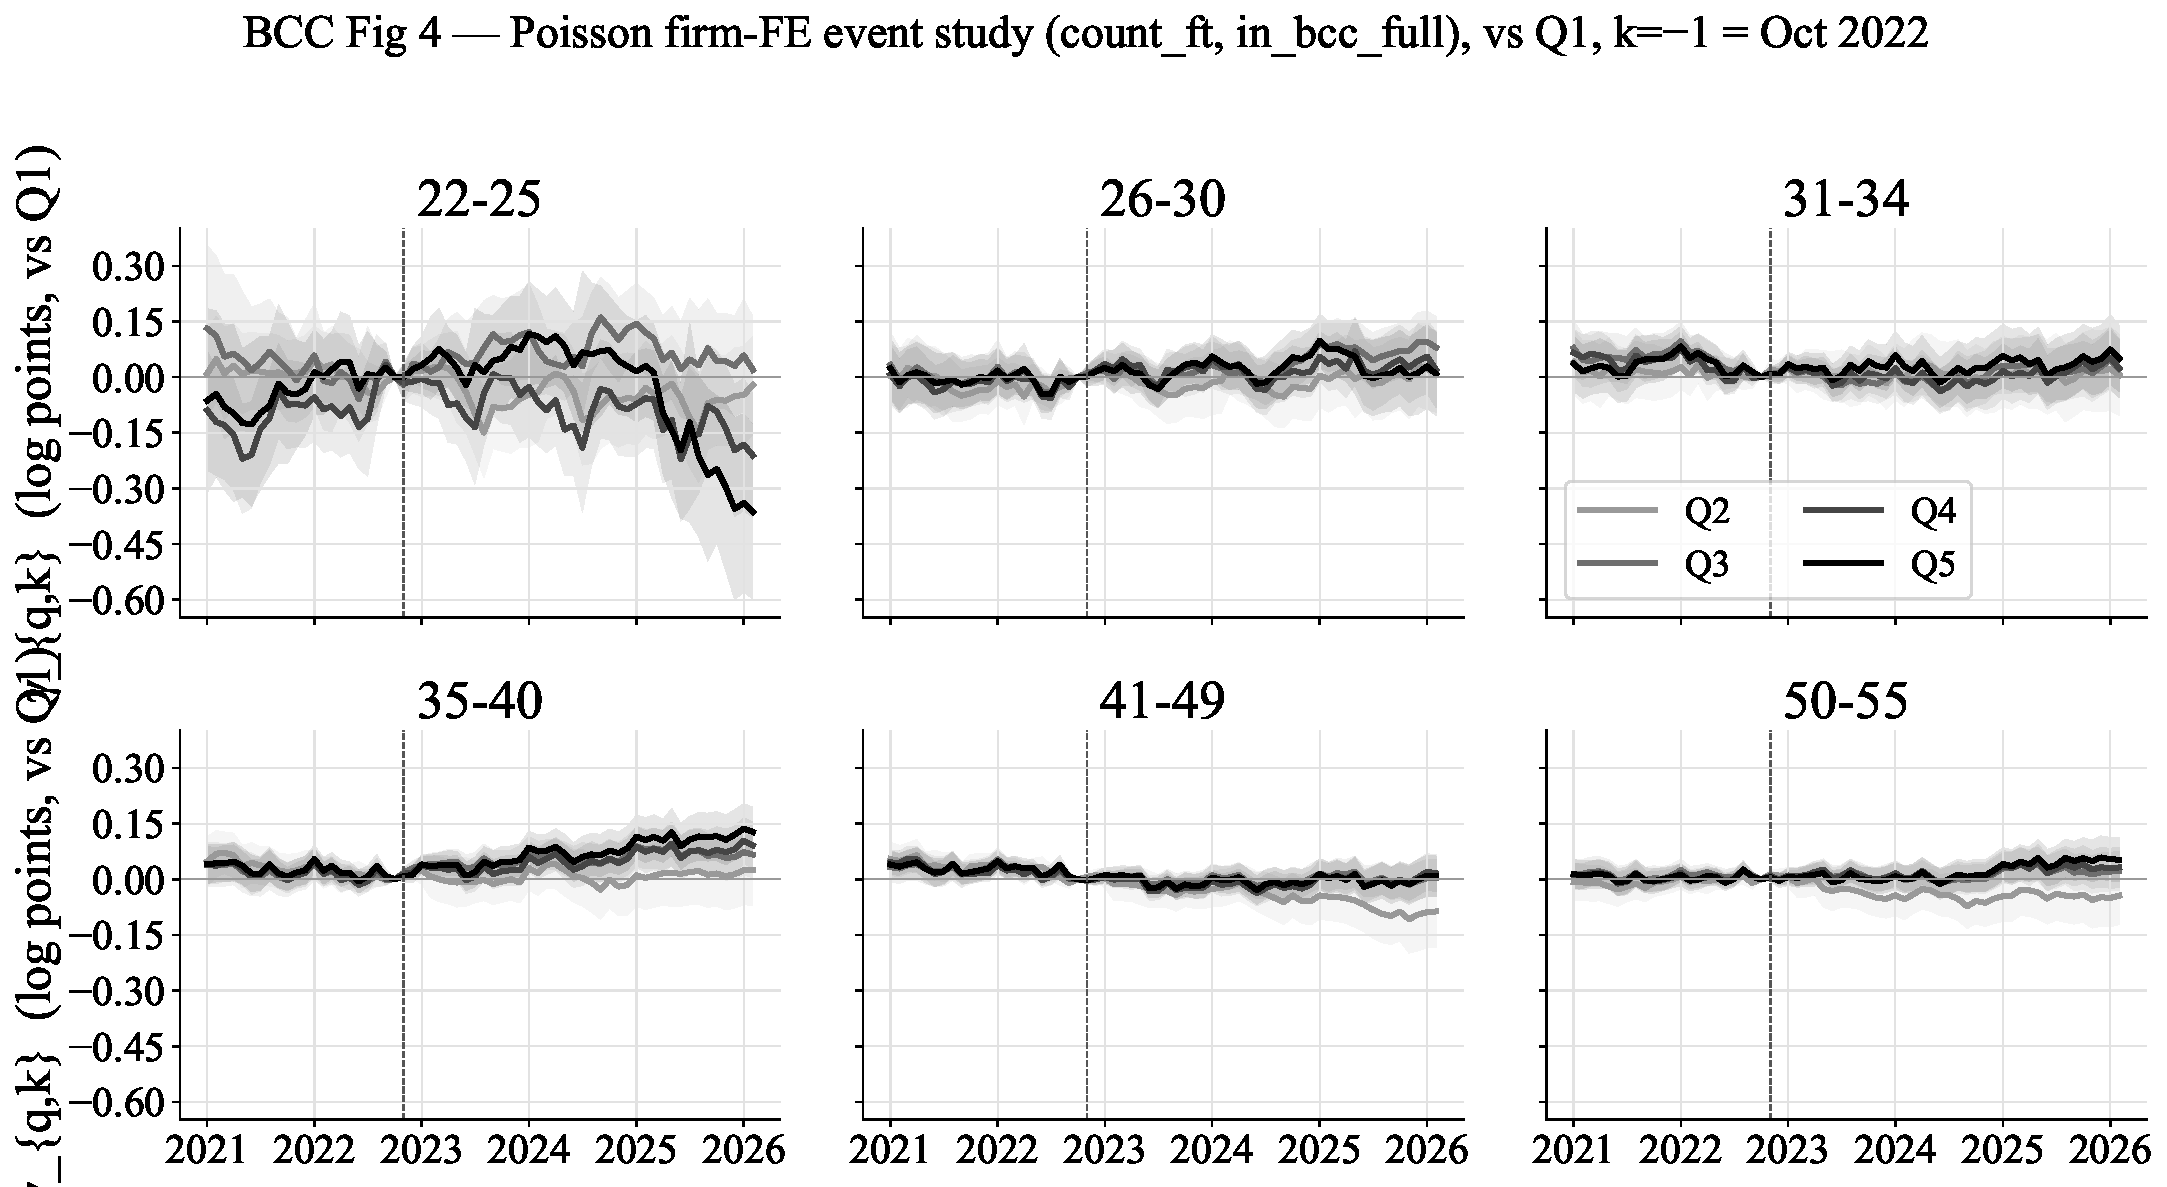
\includegraphics[width=\textwidth]{../analysis-indiv/output/bcc_appendix/fig_bcc_4_es.pdf}
  \caption{Poisson event-study coefficients, most versus least exposed quintile, by age group.}
  \label{fig:bcc_es}
  \begin{minipage}{\textwidth}\footnotesize\textit{Notes:} Q5-vs-Q1 Poisson event-study coefficients, in log points, by six age bins from 22--25 to 50--55, relative to October 2022. Firm fixed effects; standard errors clustered at the firm. Shaded bands: 95\% confidence intervals. Sample 2021m1--2026m2. Dashed line marks the November 2022 ChatGPT release.\end{minipage}
\end{figure}

\begin{figure}[htbp]
  \centering
  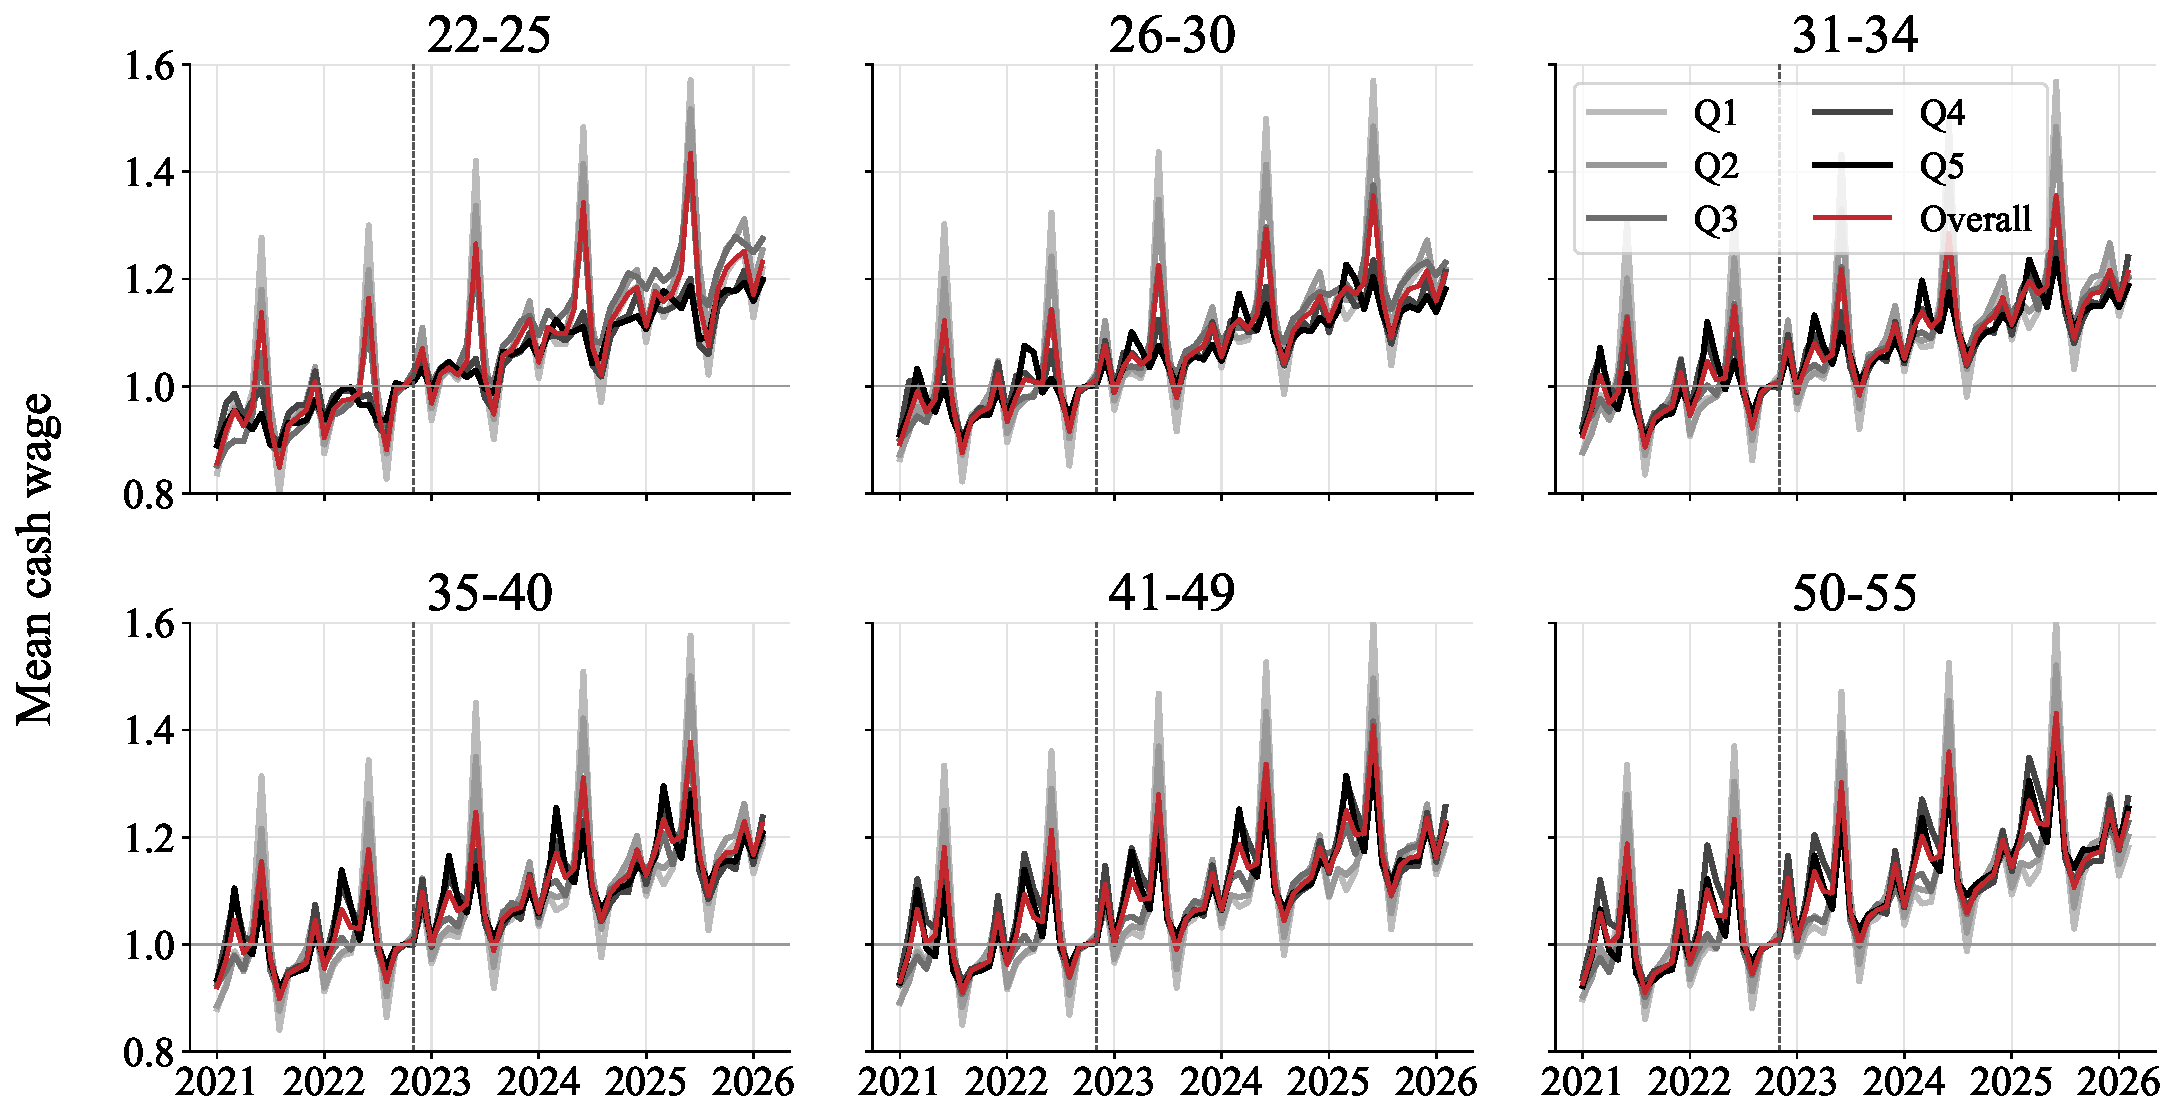
\includegraphics[width=\textwidth]{../analysis-indiv/output/bcc_appendix/fig_bcc_5_comp.pdf}
  \caption{Mean cash earnings by Eloundou exposure quintile and age group, Brynjolfsson et al.\ replication.}
  \label{fig:bcc_comp}
  \begin{minipage}{\textwidth}\footnotesize\textit{Notes:} Mean monthly cash earnings indexed to October 2022 = 1, by Eloundou GPT-4 quintile within each age group, with a pooled overall line. Full-time private-sector workers in the balanced panel.\end{minipage}
\end{figure}

\end{document}
